
\documentclass[a4paper,11pt]{article}
% Document line spacing
\usepackage{setspace}
% Maths resource packages
\usepackage{amsmath,amssymb,amsfonts,amsthm}
% Packages to allow inclusion of graphics
\usepackage{graphicx}
% Literature reference style
\usepackage[authoryear]{natbib}
\usepackage[bf]{caption}
% Display URLs correctly
\usepackage{url}
% Code display
\usepackage[outputdir=build]{minted}
\usepackage{xcolor}
% Import csv-files for tables
\usepackage{csvsimple}
% Round numbers (in tables)
\usepackage{siunitx}
% Display sideways figures (landscape mode)
\usepackage{rotating}
% Enforce line breaks
\usepackage[breakall]{truncate}
% Align decimal points in tables
\usepackage{dcolumn}
\newcolumntype{.}{D{.}{.}{-1}}
% Align footnotes (no indent of first line)
\usepackage[bottom,flushmargin,hang,multiple]{footmisc}
% Write pseudo code
\usepackage{algorithm}
\usepackage{algpseudocode}
\usepackage{etoolbox}
\usepackage{tabularx}
% Create tables with cells over multiple rows and columns
\usepackage{multirow, multicol}
% Include appendix sections in the TOC
\usepackage[toc]{appendix}
% Control behaviour of floating graphics, tables etc.
\usepackage{float}
% Correctly print "tilde" character
% \usepackage{textcomp}
% \newcommand{\textapprox}{\raisebox{0.5ex}{\texttildelow}}
% Widow and orphan control (single lines at start or bottom of page)
\usepackage[all]{nowidow}
% Create hyperlinks in cross references (for tables etc.)
\usepackage[hidelinks]{hyperref}

% -----------------------------
% --- user-defined commands ---
% -----------------------------

% insert Quantnet logo
\newcommand{\quantnet}{\raisebox{-1pt}{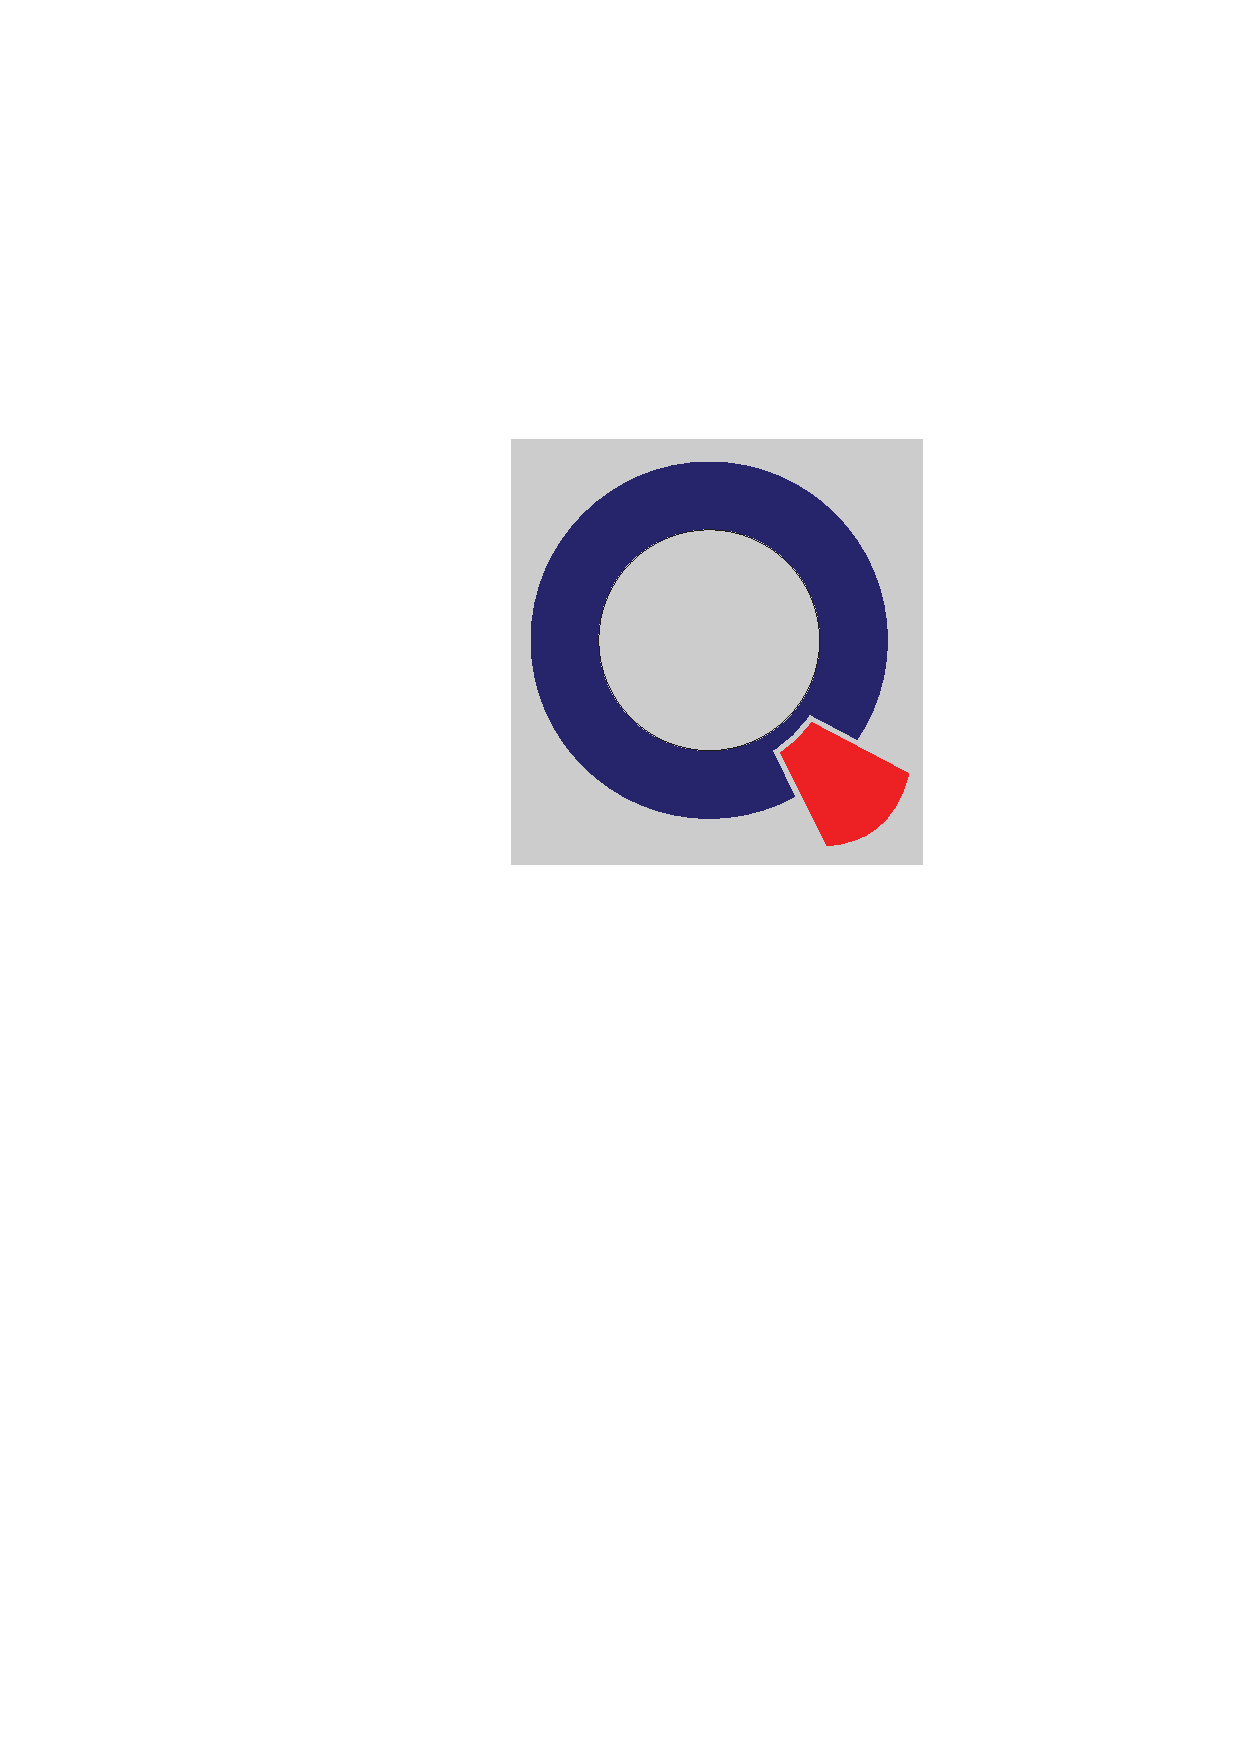
\includegraphics[scale=0.05]{thesis/figures/qletlogo.pdf}}\,}

% display vectors as bold symbols without arrow as superscript
\renewcommand{\vec}[1]{\boldsymbol{#1}}

% add possessive 's to author name in citation
\newcommand\cites[1]{\citeauthor{#1}'s\ (\citeyear{#1})}

% define arg min with underscored argument
\DeclareMathOperator*{\argmin}{\arg\min}

% enable "short" URLs without https:// or www part
\newcommand\rurl[1]{%
  \href{https://#1}{\nolinkurl{#1}}%
}

% Hyphenation of new words
\hyphenation{block-chain}

% --------------------------
% --- layout definitions ---
% --------------------------

% define topline
\usepackage[automark]{scrpage2}
\pagestyle{scrheadings}
\automark{section}
\clearscrheadings
\ohead{\headmark}

% define bibliography style
\bibliographystyle{agsm_edited}
\renewcommand{\harvardurl}[1]{URL: \url{#1}}
\renewcommand*{\UrlFont}{\itshape}

% define page size, margin size
\setlength{\headheight}{1.1\baselineskip}
\voffset=-3cm
\hoffset=-3cm
\textheight24cm
\textwidth16cm
\topmargin1cm
\oddsidemargin3cm
\evensidemargin3cm

% define line spacing = 1.5
\spacing{1.5}

% set line spacing for algorithms
\makeatletter
\expandafter\patchcmd\csname\string\algorithmic\endcsname{\itemsep\z@}{\itemsep=1.5ex}{}{}
\makeatother

% set indent manually in algorithm environment
\makeatletter
\newcommand{\multiline}[1]{%
  \begin{tabularx}{\dimexpr\linewidth-\ALG@thistlm}[t]{@{}X@{}}
    #1
  \end{tabularx}
}
\makeatother

% define space between text and footnote line
\addtolength{\skip\footins}{2pc plus 5pt}

% define space between footnotes
\setlength{\footnotesep}{1em}

% define second level for 'itemizing'
\renewcommand{\labelitemii}{-}

% Minted configuration
\definecolor{friendlybg}{HTML}{f0f0f0}

\setminted[r]{style=friendly, bgcolor=friendlybg,
breaklines, linenos}

\setminted[java]{style=friendly, bgcolor=friendlybg,
breaklines, linenos}



% ----------------------------------
% --- additional global settings ---
% ----------------------------------

% Number equations by sections
\numberwithin{equation}{section}

% Number figures by sections
\numberwithin{figure}{section}

% Number tables by sections
\numberwithin{table}{section}



% --------------------------------------
% --------------------------------------
% --------------------------------------
% --- the structure this tex document ---
% frontmatter:
%   - titlepage,
%   - acknowledgement,
%   - abstract,
%   - table of contents,
%   - list of abbreviations,
%   - list of figures,
%   - list of tables.
%
% body of the thesis:
%   - introduction,
%   - methods,
%   - data,
%   - results,
%   - conclusion,
%   - literature,
%   - appendix (figures, tables).
%
% last page:
%   - declaration of authorship.
% --------------------------------------
% --------------------------------------
% --------------------------------------




\begin{document}

% -------------------------------
% --- frontmatter: Title page ---
% -------------------------------

\thispagestyle{empty}
\begin{center}

    {\Large{\bf Forecasting in blockchain-based smart grids: Solving a prerequisite for the implementation of local energy markets}} \vspace{1cm}


    {\normalsize Master's Thesis submitted\\\vspace{0.5cm}
    to}\\\vspace{0.5cm}
    {\normalsize{\bf Prof. Dr. Wolfgang H\"ardle}} \\\vspace{0.5cm}
    {\normalsize Humboldt-Universit\"at zu Berlin \\
    School of Business and Economics \\
    Ladislaus von Bortkiewicz Chair of Statistics} \vspace{1cm}
    
    
\includegraphics[]{thesis/figures/logo.pdf}
    \vspace{1cm}

    {\normalsize by \\\vspace{0.5cm}
    {\bf Michael Kostmann} \\
    (550961)} \vspace{1cm}


    {\normalsize in partial fulfillment of the requirements \\
    for the degree of \\
    {\bf Master of Science} \\\vspace{1cm}
    Berlin, \today}

\end{center}




% -----------------------------
% --- frontmatter: Abstract ---
% -----------------------------
\newpage
\pagestyle{plain}
\pagenumbering{roman}   % define page number in roman style
\setcounter{page}{1}    % start page numbering
\section*{Abstract}

Local energy markets (LEM) have been proposed as a solution to the challenges introduced by the current transformation of the energy landscape towards more distributed and volatile energy production from renewable energy sources. Blockchain-based LEM take the proposed solution one step further and implement the market mechanism as a smart contract. This makes a central authority coordinating the LEM obsolete. The proposed blockchain-based LEM rely on accurate forecasts of individual households' energy consumption and production to trade in the LEM. In a majority of the literature, such accurate forecasts are simply assumed to be given. The present research tests this assumption by evaluating the forecast accuracy achievable with current state-of-the-art energy forecasting techniques for individual households. In a second step the effect of prediction errors made by the best performing forecasting technique on market outcomes is assessed in three different supply scenarios. The evaluation shows, that although a LASSO regression model is capable of achieving reasonably low forecasting errors, the costly settlement of prediction errors can offset and even surpass the savings brought to consumers by a blockchain-based LEM. This shows that prediction errors can make the participation in LEM uneconomical for consumers, and thus, has to be taken into consideration in future research on blockchain-based LEM.

%%%%%%%%%%%%%%%%%%%%%%%%%%%%%%%%%%%%%%%%%%%%%%%%%%%%%%%%%%%%%%%%%



% -----------------------------
% --- frontmatter: Contents ---
% -----------------------------
\newpage
\tableofcontents
\clearpage


% ---------------------
% --- Abbreviations ---
% ---------------------
\newpage
\addcontentsline{toc}{section}{List of Abbreviations}
\ohead[]{LIST OF ABBREVIATIONS}
\section*{List of Abbreviations}

%\begin{multicols}{2}
\begin{tabular}{rp{0.2cm}lp{1cm}rp{0.2cm}l}
    LEM     & &  Local energy market         & & RNN     & &  Recurrent neural network  \\
    LSTM    & &  Long short-term memory      & & LASSO   & &  Least absolute shrinkage \\
            & &                               & &         & &  and selection operator
\end{tabular}
%\end{multicols}



% ------------------------------------
% --- frontmatter: List of Figures ---
% ------------------------------------
\newpage
\addcontentsline{toc}{section}{List of Figures}
\ohead[]{\rightmark}
\listoffigures



% -----------------------------------
% --- frontmatter: List of Tables ---
% -----------------------------------
\newpage
\addcontentsline{toc}{section}{List of Tables}
\listoftables



% -------------------------------
% --- main body of the thesis ---
% -------------------------------
\newpage
\pagestyle{plain}
\setcounter{page}{1}    % start page numbering anew
\pagenumbering{arabic}  % page numbers in arabic style

\section{Introduction}\label{Sec:Intro}



%%%%%%%%%%%%%%%%%%%%%%
%%%   Motivation   %%%
%%%%%%%%%%%%%%%%%%%%%%

\subsection{Motivation}\label{Sec:Intro;Subsec:Motivation}

The increasingly wide-spread installation of renewable energy generators currently transforms the German energy landscape substantially \citep{Bayer:2018}. Already in 2017, more than 1.6 million photovoltaic micro-generation units were installed in Germany, according to the Bundesverband Solarwirtschaft \citeyearpar{BSW-Solar:2018}. This increasing amount of distributed renewable energy resources combined with a more volatile energy consumption of households –-- e.g., due to uncontrolled electric vehicle charging that can increase peak consumption \citep{Fitzgerald:2016,Floch:2017} --– presents a serious challenge for grid operators. As energy production and consumption have to be balanced at all times in any electricity grid \citep{Weron:2006}, the increasingly volatile and hard to predict energy consumption and production in low voltage grids requires new technological solutions to manage grid load and energy distribution.

Fortunately, the technological advancement that lead to the increasing complexity in the energy landscape, also opens up new opportunities to increase the efficiency and reliability of distributed renewable energy production and distribution. As the amount of renewable energy production, that is fed into low voltage grids, has been increasing over the last years \citep{Bayer:2018}, it seems reasonable to shift part of the grid management to lower grid levels. While industry and research already established a comprehensive set of grid management solutions as well as sophisticated consumption and production forecasting techniques for highly aggregated levels, there is still little research on the same topics at lower aggregation levels, such as neighbourhoods or even individual households \citep{Meer:2018}.

One rather recent technological advancement that has the potential to increase the level of energy distribution efficiency on low aggregation level is the implementation of local energy markets on a distributed ledger technology such as blockchain. Blockchain has been called an invention similarly revolutionary and paradigm shifting as the internet \citep{Swan:2015}. While much of the hype around blockchain still has to stand the test against reality, the technology undeniably has the potential to enable new technological solutions. It is not for no reason that more than 20~\% of 70 surveyed German energy executives believe blockchain will be “a game changer for the energy industry” and further 60~\% believe further dispersion of blockchain technology is probable \citep{Burger:2016}. A use case that has been getting special attention due to the media-effective inauguration of the Brooklyn Microgrid \citep{newscientist:2016} are blockchain-based local energy markets.

Local energy markets (LEM) enable localized interconnected energy consumers, producers, and prosumers to trade locally produced energy\footnote{In this thesis, the terms energy and electricity are used interchangeably as is common in related literature. However, to be precise, the term energy comprises electricity and heat and a local energy market does not necessarily has to be constrained to the trading of electricity. Still, all further mentions of the term ``energy'' in this work refer to electricity.} on a market platform with a specific pricing mechanism \citep{Mengelkamp:2018a}. A common pricing mechanism used for this purpose are discrete double auctions \citep{Lamparter:2010, Buchmann:2013, Block:2008}.  Blockchain-based LEM utilize a blockchain as underlying information and communication technology and a smart contract to match supply and demand and settle transactions \citep{Mengelkamp:2018b}. As a consequence, a central authority that coordinates the market is obsolete in a blockchain-based LEM. Major advantages of such LEM are (near) real-time pricing \citep{Mihaylov:2014}, balancing of energy production and consumption in local grids \citep{Stadler:2016}, and lower energy costs for consumers \citep{Mengelkamp:2018agentstrategies}. Further advantages include more customer choice (empowerment) \citep{Koirala:2016} and less power line loss due to long transmission distances \citep{Hvelplund:2006}.

However, the product traded on energy markets has some peculiarities compared to other goods. First, energy grids always have to be balanced, i.e., energy demand always has to be matched by energy supply \citep{Weron:2006}. Secondly, as energy is difficult to store, produced energy is fed into the grid mostly instantaneously and continuously and cannot be exchanged in batches of a specific amount at a single point in time \citep{Rosen:2013}. Traditionally, this means that the aggregated energy demand for a geographic area and a specific period of time has to be forecasted and, according to this forecast, energy is bought and sold. The actual electricity production is then managed to continuously match the current demand \citep{Rosen:2013}. This setting is the reason for today’s existing energy landscape, where utilities and large-scale energy producers and consumers are the only agents involved in electricity markets \citep{Weron:2006, Buchmann:2013}. They trade energy according to the aggregated demand of many consumers. This aggregation makes forecasting future energy demand with relatively small errors \citep{Meer:2018, Wang:2018} and thereby efficient trading possible. Household-level consumers or prosumers, however, do not actively trade but pay their consumption or are reimbursed for their infeed of energy into the grid according to preset tariffs \citep{Rosen:2013}. 

In LEM, on the contrary, households are the participating market agents that typically submit offers in an auction design \citep{Ilic:2012, Lamparter:2010}. Due to the non-storability of the traded good, the participating households need to forecast their energy demand, respectively supply, to be able to submit a buy or sell offer to the market \citep{Rosen:2013}. Therefore, accurate forecasts are a necessary precondition for such market designs. However, even though forecasting is substantially harder for single households compared to higher aggregation levels \citep{Wang:2018}, in existing research on (blockchain-based) LEM, it is frequently assumed such accurate forecasts are readily available \citep{Rosen:2013, Mengelkamp:2018c, Lamparter:2010, Buchmann:2013, Mengelkamp:2018a}. This assumption may not be correct and given the substantial uncertainty in individual households' energy consumption or production, prediction errors may have a significant impact on market outcomes.

Thus, the present research aimed to evaluate the possibility of providing such reasonably accurate forecasts with existing methods and currently available smart meter data. Moreover, it aimed to quantify the effect of prediction errors on market outcomes in blockchain-based LEM. As such, this has not been done in previous literature. However, for the future advancement of the field it seems imperative that the precondition of accurate forecasts of individual households' energy consumption and production for LEM is sufficiently assessed. Only then, the assumption of readily available accurate forecasts can be -- if necessary -- adjusted in future work.

%%%%%%%%%%%%%%%%%%%%%%%%%%%%
%%%   Related research   %%%
%%%%%%%%%%%%%%%%%%%%%%%%%%%%

\subsection{Related research}\label{Sec:Intro;Subsec:Related}
The present work's topic of concern touches upon three superordinate fields of research. The first field is local energy markets, their market structure, market mechanism, and market outcomes as well as possible advantages and disadvantages. The second field is distributed ledger technology (here, that is, blockchain and smart contracts) and its use cases for different fields. The third field is energy forecasting, which encompasses energy consumption forecasting and energy production forecasting. Especially the latter has attracted a lot of attention in the light of the increasing adoption of renewable energy resources. All this comes together in blockchain-based LEM as, for example, implemented in the Brooklyn Microgrid and simulated by \citet{Mengelkamp:2018a}. The following sections give a brief overview on related research that is relevant for the present research.



%%%%%%%%%%%
\subsubsection{Local energy markets}

Although, local energy markets started to attract interest in academia already in the early 2000s, it is still an emerging field according to \citet{Stadler:2016}. Early work by \citet{Alibhai:2004}, for example, describes auctions as a coordination mechanism for microgrids. In their setting, energy producers within the market bid on requested electricity amounts by consumers. They compare different auction designs and come to the conclusion that Dutch auctions are the most preferable for their application. \citet{Block:2008} are one of the few studies specifically referring to electricity and heat in their design of a local energy market. They propose a combinatorial double auction that sets a uniform equilibrium price in discrete time intervals and analytically develop a open book call market utilizing an arbitrage agent and spinning reserves to stabilize the local market. Other early work mainly focused on microgrids in island mode (i.e., autarchic and disconnected from a superordinate grid, such as on remote islands) and the setting of a uniform market clearing price in single-sided and double-sided auction designs \citep{Sinha:2008}. While this is especially interesting for developing regions, more recent work shifted focus on use cases in developed and highly technologized energy grid systems. This is mainly driven by the wide spread adoption of smart meters and internet-connected home appliances \citep{Burger:2016}.

For example, \citet{Lamparter:2010} introduce a fully flexible and modular market platform that coordinates market agents through a mechanism that incentivizes truthful policy revelation (i.e., bidding behaviour). The software platform they developed uses a double auction (Vickrey-Clark-Groves auction) that allows for divisible bids to achieve highly efficient market outcomes. A market mechanism that is applied in a real world project is developed by \citet{Ilic:2012}. Again, a double auction with discrete time slots is used to achieve a high market efficiency with price behaviour that conforms to standard economic theory. Using almost the same market mechanism and very similar simulation design, \citet{Buchmann:2013} focus on a new aspect that will most likely become more important in future applications of LEM: They tackle the problem of lacking privacy that is present in any LEM conforming with current German energy trading regulation. Using common anonymization methods they show that protecting the privacy of trading agents comes only at moderate cost in terms of higher prices and lower market efficiency. \citet{Rosen:2013} on the other hand bring up the important aspect of easy understandability that is needed for successful implementations of LEM and focus on establishing a market mechanism that is appropriate also in settings with few market participants. This is especially in early stages of LEMs an often neglected but all the more important aspect.

The work of \citet{Buchmann:2013} and \citet{Rosen:2013} show that the research has moved to a point were practical implementability of LEM becomes a key concern. This focus is also present in a series of several studies that assess the usefulness of automated trading agents. Comparing zero intelligence and intelligent trading agents in two different market scenarios, \citet{Mengelkamp:2017:Trading} establish the general usefulness of automated trading agents to achieve efficient market outcomes. This work is extended in \citet{Mengelkamp:2018:Clustering} that demonstrates the feasibility of representing household preferences with intelligent trading agents. \citet{Mengelkamp:2018c} then improve the performance of the intelligent trading agents employing reinforcement learning in a short-term merit order market mechanism.



%%%%%%%%%%%
\subsubsection{Blockchain and smart contracts}

The recently renewed research interest in LEM appeared more or less simultaneously to the exploding interest in the revolutionary distributed ledger technology, most notably blockchain \citep{Swan:2015}. As the focus of the present research does not require a detailed understanding of distributed ledger technology, a in-depth explanation of its functioning is not required here. In short, blockchain can be described as a distributed record keeper (a "ledger", i.e., a database) that records transaction between participating agents, called nodes \citep{Burger:2016}. Distributed here means that a copy of the same database (or a shortened version) is stored on each node. Summarizing \citet{Tapscott:2016}, each transaction that is executed on a blockchain is added to a so-called block. Each block contains a fixed number of transactions and has to be verified by a majority of participating nodes to be added ("chained") to the distributed ledger. This addition is secured through cryptography. That means, any party trying to manipulate previous transactions would have to change all subsequent blocks of the blockchain on a majority of the participating nodes. As this would be computationally extremely demanding, it is extremely unlikely, giving blockchain its lauded characteristics of unalterability and secureness \citep{Burger:2016}.

For the present research, a variant of the original blockchain technology is relevant: Ethereum is an open source platform built on blockchain technology. It can serve as infrastructure for any kind of blockchain-based application, cryptocurrency, protocol, and the like. On the Ethereum blockchain, any kind of programmable task can be implemented in an immutable, transparent, and distributed way. Due to the open source nature of Ethereum it is possible to “clone” the public Ethereum blockchain onto a private machine and use it as a private blockchain for simulation, testing or closed commercial applications. \citep{Ethereum:2018doc, Swan:2015}.

Another closely related term often mentioned in combination with blockchain technology is "smart contract". The concept and term smart contract dates back to Nick Szabo, who defined a smart contract as “a computerized transaction protocol that executes the terms of a contract” \citep{szabo:1994}. Simplified, a smart contract can be described as software or hardware that represents contractual clauses and can automatically register and initialize the fulfilment of its terms while penalizing a contracting party in case of any violation of the contract \citep{Szabo:1997}. For example, this contractual clauses could represent a market mechanism that is used to trade energy in a local market. As such it is implemented by \citet{Mengelkamp:2018a}.


%%%%%%%%%%%
\subsubsection{Blockchain-based local energy markets}

While substantial work regarding LEM in general has been done, there are only few examples of blockchain-based LEM designs in the existing literature. \citet{Mengelkamp:2018b} derive seven principles for microgrid energy markets and evaluate the Brooklyn Microgrid according to those principles. According to the authors knowledge, they are the only ones providing a theoretical framework for the design of blockchain-based LEM and their work may serve as the basis for the future research and implementation of such energy markets.

With a more practical focus, \citet{Mengelkamp:2018a} implemented and simulated a local energy market on a private Ethereum-blockchain that enables participants to trade local energy production on a decentralized market platform with no need for a central authority. \citet{Münsing:2017} similarly elaborate a peer-to-peer energy market concept on a blockchain but focus on operational grid constraints and a fair payment rendering. In doing so, they present a decentralized optimal power flow model suitable for the implementation on a blockchain.

Outside of academia however, there are several undertakings to put blockchain-based energy trading into practice. Prominent examples of such projects are, among others, Grid Singularity (\rurl{gridsingularity.com}) in Austria, Powerpeers (\rurl{powerpeers.nl}) in the Netherlands, Power Ledger (\rurl{powerledger.io}) in Australia, and LO3 Energy (\rurl{lo3energy.com}) in the US.



%%%%%%%%%%%
\newpage
\subsubsection{Load forecasting for individual households}


For blockchain-based LEM, as the one simulated by \citet{Mengelkamp:2018a}, a necessary prerequisite is the successful forecast of household-level energy consumption respectively production based on smart meter recordings. Without this, trading through an auction design as described in, e.g., \citet{Block:2008} or \citet{Buchmann:2013}, and implemented in a smart contract by \citet{Mengelkamp:2018a} is not possible. This forecasting task is not trivial due to the extremely high volatility of individual households' energy patterns \citep{Wang:2018}. Nevertheless, there are several studies trying to forecast different time horizons of smart meter time series.

\citet{Arora:2016} compute probability density estimates for the electricity consumption recorded by individual smart meters in halfhourly intervals from 1000 households and SMEs in Ireland over the course of one year. They employ unconditional and conditional kernel density estimators with a decay parameter to generate point and density forecasts for electricity consumption from 30 minutes to one week ahead. \citet{Kong:2018} use a long short-term memory deep learning framework to make one time-step ahead forecasts on the AMPds data set containing half-hourly recordings of energy and appliance usage measurements of a single household in Canada. They show that the prediction accuracy can be improved substantially by including appliance measurement data. On the same data set as \citet{Arora:2016}, \citet{Shi:2017} use a pooling-based deep recurring neural network to make point forecasts of future consumption and achieve substantial mean absolute percentage error reductions compared to ARIMA, recurring neural network, support vector machine, and deep recurring neural network approaches. Even though focusing on the forecast of aggregated energy consumption, the work of \citet{Zufferey:2017} shows promising results for forecasting smart meter time series with time delay neural networks using mostly historical features of the time series itself. They use a huge data set of 40.000 small consumers and 400 photovoltaic power generators in Basel, Switzerland with 15-minutes interval recordings of energy consumption and production for one year.

Contrary to these machine learning approach, \citet{Li:2017} use statistical methods to make one time-step ahead forecasts with a sparse autoregressive LASSO model. Using a data set of 150 consumers from PG\&E with hourly energy consumption recordings for one year, their model captures sparsity in the household’s historical data via LASSO to make a prediction for one household. This prediction is further improved with the historical consumption data of one additional household. This household is identified with the help of a covariance statistic test to identify one other household's data that has the best predictive leverage to improve the original forecast.

A comprehensive overview on the state-of-the-art of smart meter data analytics is provided by \citet{Wang:2018}. The authors do not only focus on studies researching load forecasting but also provide comprehensive insights into studies regarding smart meter data clustering, preprocessing, load analysis and more. Furthermore, they provide a summary of publicly available smart meter data sets and open research topics. Notably, there is a lack of standard regarding which forecasting error measures are reported and what benchmark models are used in smart meter data forecasting studies. This is also pointed out by \citet{Meer:2018} in their review paper on probabilistic consumption and production forecasting. Due to this, different forecasting techniques employed in studies using different data sets, with partly differing objectives, and different inputs are not directly comparable. 



%%%%%%%%%%%%%%%%%%%%%%%%%%%%
%%%   Present research   %%%
%%%%%%%%%%%%%%%%%%%%%%%%%%%%
\subsection{Present research}\label{Sec:Intro;Subsec:Present}

The objective of this Master's thesis was to investigate the prerequisites necessary to implement blockchain-based distributed local energy markets. In particular this meant
\begin{itemize}
    \item[a)] forecasting net energy consumption respectively production of private consumers and prosumers one time-step ahead based only on the historical consumption respectively production data (and potentially calender features),
    \item[b)] evaluating and quantifying the effects of forecasting errors, i.e., deviations between forecasted and actual consumption respectively production, for households participating in a LEM, and
    \item[c)] evaluating the implications of low forecasting quality for a market mechanism that includes a settlement mechanism for forecasting errors.
\end{itemize}

The underlying setting and technical implementation of the LEM that was assumed for the present research, is provided by \citet{Mengelkamp:2018a}. The prediction task was fitted to their setup of a LEM that uses blockchain technology as its information and communication medium. Thereby, the present research distinguishes itself notably from previous studies that solely try to forecast smart meter time series in general. The evaluation of forecasting errors and their implications was based on the commonly used market mechanism of discrete interval, double sided auctions \citep[e.g.,][]{Block:2008, Buchmann:2013}, while the forecasting error settlement structure was based on \citep{Mengelkamp:2018a}. As such, to the authors knowledge, an assessment of the effect of prediction errors on market outcomes has not been done in previous studies. Accordingly, the following research questions were examined in the present research:
\begin{itemize}
    \item[a)] Which prediction technique yields the best 15-minutes ahead forecast  for smart meter time series measured in 3-minutes intervals using only input features generated from the historical values of the time series and calendar-based features?
    \item[b)] Assuming a forecasting error settlement structure as described in \citet{Mengelkamp:2018a}, what is the quantified loss of households participating in the LEM due to forecasting errors by the prediction technique identified in a)?
    \item[c)] Depending on the results from b), what implications and potential adjustments for the market mechanism described in \citet{Mengelkamp:2018a} can be identified?
\end{itemize}

The remainder of the present research is structured as follows: Section~\ref{Sec:Method} presents the forecasting models and error measures used to evaluate the prediction accuracy. Furthermore, it introduces the market mechanism and the implementation of the market simulation which was used to evaluate the effect of prediction errors on market outcomes. Thereafter, Section~\ref{Sec:Data} describes in detail the data used for this study. As the data has not been used in previous studies, emphasis is put on exposing the characteristics and potential peculiarities of the data at hand. Section~\ref{Sec:Results} presents the prediction results of the forecasting models, evaluates their performance relative to a benchmark model and assesses the effect of prediction errors on market outcomes. The insights gained from this are then be used to identify implications and potential adjustments for future market mechanisms that could be implemented as smart contract in a blockchain. Finally, Section~\ref{Sec:Conc} concludes with a summary, limitations, and an outlook on further research questions that emerge from the findings of the present research.

%%%%%%%%%%%%%%%%%%%%%%%%%%%%%%%%%%%%%%%%%%%%%%%%%%%%%%%%%%%%%%%%%

\newpage

\section{Methods}\label{Sec:Method}

Based on an extensive literature review which is very briefly summarized in Section~\ref{Sec:Intro;Subsec:Related}, two different forecasting techniques were chosen to be employed to predict households' energy consumption and production. The following criteria were considered for the selection of appropriate methods: 

\begin{enumerate}
    \item The forecasting technique has to produce deterministic (i.e., point) forecasts.
    \item The forecasting technique had to be used in previous studies about forecasting energy consumption or production.
    \item The previous study or studies using the forecasting technique had to use comparable data, i.e., recorded by smart meters in 60-minutes intervals or higher resolution, recorded in multiple households, and not recorded in SMEs or other business or public buildings.
    \item The forecasting task had to be comparable to the forecasting task of this study, i.e., single consumer household (in contrast to the prediction of aggregated energy time series) and very short forecasting horizon ($\leq 24$ hours).
    \item The forecasting technique had to only take historical and calender features as input for the prediction.
    \item The forecasting technique had to produce absolutely and relative to other studies promisingly accurate predictions.
\end{enumerate}

\noindent Based on these criteria two forecasting techniques were selected for the prediction task at hand. As short-term energy forecasting techniques are commonly categorized into statistical and machine learning (or artificial intelligence) methods \citep{Bansal:2015,Diagne:2013,Gan:2017}, one method of each category was chosen: Long short-term memory recurrent neural network (LSTM RNN) adapted from the procedure outlined by \citet{Shi:2017} and sparse autoregressive LASSO as developed and implemented by \citet{Li:2017}.

Before these two methods are explained in detail, the benchmark model, that serves as a baseline for the assessment of the prediction methods, is presented next. Thereafter, the two prediction methods are elaborated. Lastly, the implementation of the market simulation is explained.


%%%%%%%%%%%%%%%%%%%%%%%%%%%
%%%   Benchmark model   %%%
%%%%%%%%%%%%%%%%%%%%%%%%%%%

\subsection{Benchmark model} \label{Sec:Method;Subsec:Benchmark}

Benchmark models serve as a trivial baseline to assess the relative improvement of a sophisticated model \citep{Meer:2018}. According to \citet{Pinson:2012}, a benchmark model should serve as a reference, need few computational resources to be estimated, and be model-free. A sophisticated forecasting method is only worth implementing if it can significantly outperform a trivial benchmark model \citep{Diagne:2013}. A frequent benchmark model used for deterministic forecasts is the simple persistence model \citep{Meer:2018}. This model assumes that the conditions at time $t$ persist at least up to the period of forecasting interest at time $t+h$. In energy forecasting, this na\"ive model is surprisingly well suited to forecast very short time periods of a few seconds or minutes \citep{Pinson:2012} and, thus, often harder to beat than it might seem. Here, the persistence model is defined as
%
\begin{equation} \label{Eq:naivepred}
\widehat{x}_{t+1}=x_t.
\end{equation}

There are several other benchmark models commonly used in energy load forecasting. Most of them are, in contrast to the persistence model, more sophisticated benchmarks, such as the Holt-Winters-Taylor (HTW) exponential smoothing method \citep[see, e.g.,][]{Arora:2016}. Further sophisticated benchmark models are the Vanilla benchmark \citep{hong:2010}, and the popular ARMA method \citep{Box:1990}. However, as the forecasting task at hand serves the specific use case of being an input for the bidding process in a blockchain-based local energy market, the improvement of the forecasting model over a benchmark model is of secondary importance. The task here is not so much to establish the quality of a forecasting model per se as to assess whether the available and most promising forecasting techniques can deliver accurate enough results for the use case explained above. Hence, only the persistence model will serve as a benchmark to the forecasting techniques presented next. The more relevant test of the forecasting models' accuracy will be explained in Section~\ref{Sec:Method;Subsec:Market}.



%%%%%%%%%%%%%%%%
%%%   LSTM   %%%
%%%%%%%%%%%%%%%%

\subsection{Machine learning based forecasting approach} \label{Sec:Method;Subsec:LSTM}

The first sophisticated forecasting technique that is employed to produce as accurate as possible predictions for the blockchain-based LEM is a machine learning algorithm. Even though being applied very successfully in a wide range of tasks, such as speech recognition \citep{Graves:2013} or anomaly detection in time series \citep{Malhotra:2015}, long short-term memory (LSTM) neural networks have been introduced only very recently in load forecasting studies \citep[e.g.,][]{Kong:2018,Shi:2017,Gan:2017,Chen:2018}. Compared to previous attempts using machine learning techniques, the applications of LSTM neural networks for load forecasting have been much more successful \citep{Kong:2018,Shi:2017}. This is most likely due to the high effectiveness of recurrent neural networks for sequence learning. LSTM neural networks are a nadvanced architecture of recurrent neural networks that are particularly well suited to learn long sequences or time series due to their ability to retain information over many time steps \citep{Chollet:2018}. The next three sections explain the basic working principles of the chosen machine learning approach and are based on \citet{Chollet:2018}, \citet{Lipton:2015}, and \citet{Gan:2017}.



%%%%%%%%%%%
\subsubsection{Basic functioning of neural networks}

To understand the full advantage that LSTM recurrent neural networks have over other machine learning techniques for time series learning, it is useful to take a step back and recapitulate the basic functioning of a so-called feedforward neural network. Neural networks do not need any strong assumptions about their functional form, such as traditional time series models (e.g., ARMA). Still, they are universal approximators for finite input \citep{Hornik:1989} and, therefore, especially well suited for the prediction of such volatile time series as energy consumption or production. The most basic building blocks of any neural network are three types of layers: an input layer, one or more hidden layer(s), and an output layer. Each layer consists of one or more units (sometimes called neurons). Each unit in a layer takes in an input, applies a transformation to this input, and outputs it to the next layer (see Figure~\ref{Fig:simpleNN}). Formally, this can be written as
%
\begin{equation} \label{Eq:feedforward}
\begin{split}
    \vec{h}_{1,i}&=\phi_1\left(\vec{W}_1\vec{x}_i+\vec{b}_1\right)\\
    \vec{h}_{2,i}&=\phi_1\left(\vec{W}_2\vec{h}_{1,i}+\vec{b}_2\right)\\
    &\setbox0\hbox{=}\mathrel{\makebox[\wd0]{\hfil\vdots\hfil}}\\
    o_i&=\phi_n\left(\vec{W}_n\vec{h}_{(n-1),i}+\vec{b}_n\right)=\widehat{y}_i,
\end{split}
\end{equation}
%
where $n$ denotes a layer, $\phi_n$ is the activation function, $\vec{W}_n$ is the weight matrix, and $\vec{b}_n$ the bias vector in layer $n$. $\vec{x}_i$ is the $i^{th}$ input vector and $o_i$ the output value of the output layer which is the estimation of the true value $y_i$.
%
\begin{figure}[htbp]
    \centering
    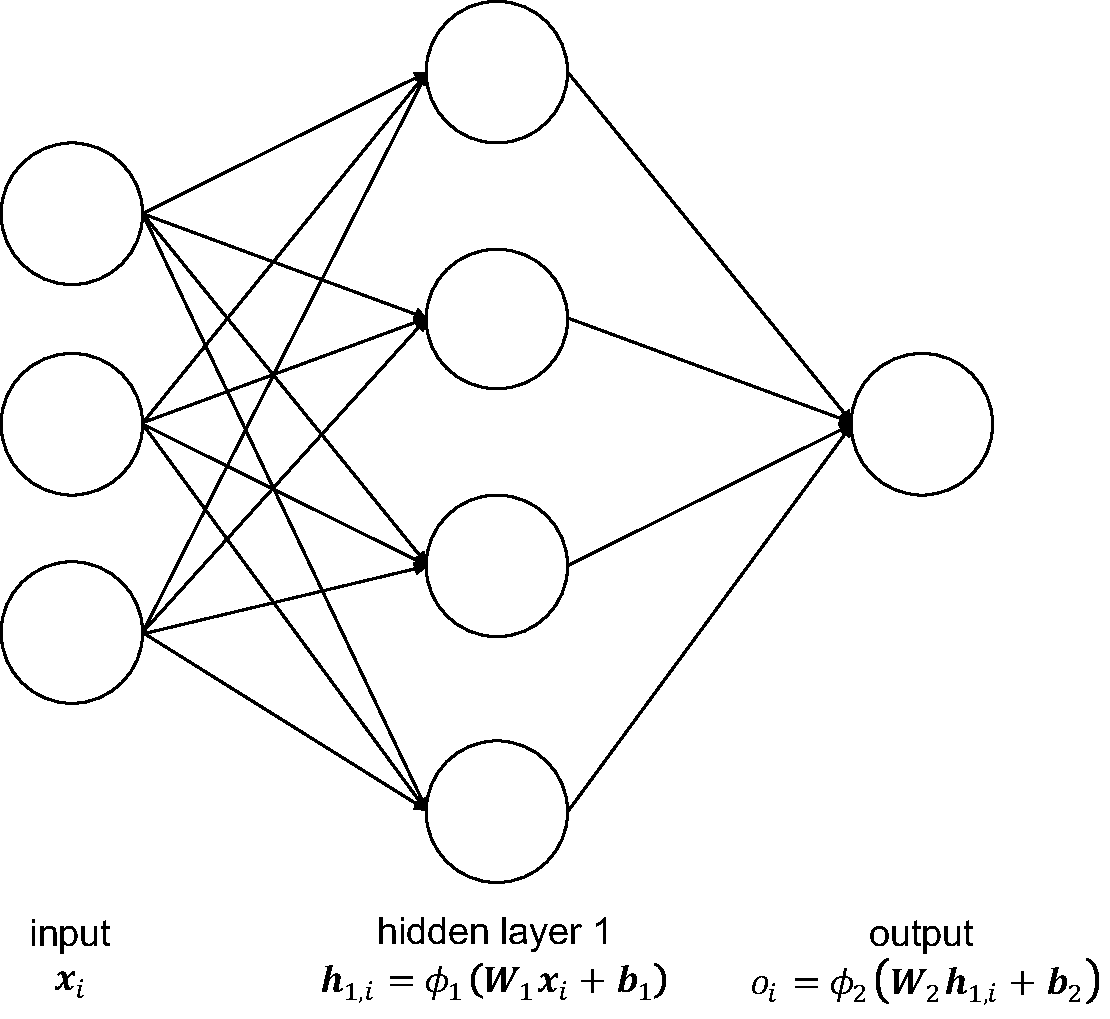
\includegraphics[scale=0.5]{thesis/figures/simpleNN.pdf}
    \caption[Schematic representation of a simple neural network]{Schematic representation of a simple neural network. Adapted from \citet{Gan:2017}.}
    \label{Fig:simpleNN}
\end{figure}

In the input layer there are as many units as there are features (i.e., variables) that serve as input for the forecasting model. The units of the input layer are connected to all units in the (first) hidden layer. The weight matrices and bias vectors in each layer are parameters that are adjusted during the training of the model. In all subsequent hidden layers, all units of the previous layer are connected to all units of the subsequent layer (this is called densely connected). The last layer consists of as many units as there are output values. That is, if the forecasting model should just predict a single value, the output layer will have a single unit that takes in the weighted output values of all units of the last hidden layer, applies a transformation to these inputs and outputs a single value. The transformation that is applied to the input within each unit is called activation function and must be chosen depending on the task at hand. Especially for sequence learning, this activation function is often a hypberbolic tangent (tanh) \citep{Lipton:2015}:

\begin{equation} \label{Eq:activation}
    \phi(z)=\frac{e^z-e^{-z}}{e^z+e^{-z}}.
\end{equation}

The learning in machine learning refers in the case of neural networks to adjusting the weight matrices and bias vectors such that the best prediction is output. In supervised learning, adjusting these weights (i.e., the training of the model) is done through an algorithm that is called backpropagation which was introduced by \citet{Rumelhart:1986}. First, the weight matrices and bias vectors are randomly initialized. Then, in a first iteration, the training data is fed into the network, which outputs a prediction. This prediction is assessed with the help of a loss function that quantifies the distance between the prediction and the true value. A commonly used loss function is the mean absolute error:
%
\begin{equation} \label{Eq:lossMAE}
    L\left(y, \widehat{y}\right)=\text{MAE}=\frac{1}{N}\sum_{i=1}^N\left|\widehat{y}_i-y_i\right|
\end{equation}
%
The simplest method to optimize the model parameters is to compute the derivative of the loss function with respect to each parameter in the model and change each parameters in a fixed-size step in the direction of the negative gradient \citep{Graves:2013}. This method is called gradient descent. Thereby, the prediction error is ``backpropagated" through the network to update the parameters. This is repeated in each iteration until the model converges to a value of the loss function that cannot be further improved.



%%%%%%%%%%%
\subsubsection{Recurrent neural networks}

Unfortunately, feedforward neural networks are not particularly well-suited for time series learning \citep{Chollet:2018}. This is because simple neural networks, such as the one described above, do not have an internal state that could retain a memory of previously processed input. That is, to learn a sequence or time series, a feedforward neural network would always need the complete time series as a single input. It cannot retain a memory of something learned in a previous chunk of the time series to apply it to the next chunk that is fed into the model. This problem is tackled by recurrent neural networks.

Recurrent neural networks still consist of the basic building blocks of units and layers. However, the units do not just feed forward the transformed input as output but have a recurrent connection that feeds an internal state back into the unit as input (see Figure~\ref{Fig:RNNunit}). Thereby, a RNN unit loops over individual elements of an input sequence, instead of processing the whole sequence in a single step. This means, the RNN unit applies the transformation to the first element of the input sequence and combines it with its internal state. This introduces the notion of time into neural networks. Formally, this can be written as
%
\begin{equation} \label{Eq:RNN}
\begin{split}
    \vec{h}_{1,t}&=\phi_1\left(\vec{W}_1^{(i)}\vec{x}_t+\vec{W}^{(r)}_1\vec{h}_{1,(t-1)}+\vec{b}_1\right)\\
    \vec{h}_{2,t}&=\phi_2\left(\vec{W}_2^{(i)}\vec{h}_{1,t}+\vec{W}^{(r)}_2\vec{h}_{2,(t-1)}+\vec{b}_2\right)\\
    &\setbox0\hbox{=}\mathrel{\makebox[\wd0]{\hfil\vdots\hfil}}\\
    o_t&=\phi_n\left(\vec{W}_n^{(i)}\vec{h}_{(n-1),t}+\vec{b}_n\right)=\widehat{y}_t,
\end{split}
\end{equation}
%
where $n$ denotes a layer, $\phi_n$ is the activation function, $\vec{W}_n^{(i)}$ is the weight matrix for the input, $\vec{W}_n^{(r)}$ is the weight matrix for the recurrent input (i.e., the output of layer $n$ in the previous time step), and $\vec{b}_n$ the bias vector in layer $n$. $\vec{x}_t$ is the input vector at time $t$ and $o_t$ the output value of the output layer which is the estimation of the true value $y_t$. Note that the output layer has no recurrent units but is the same as in a simple feed forward network.
%
\begin{figure}[htbp]
    \centering
    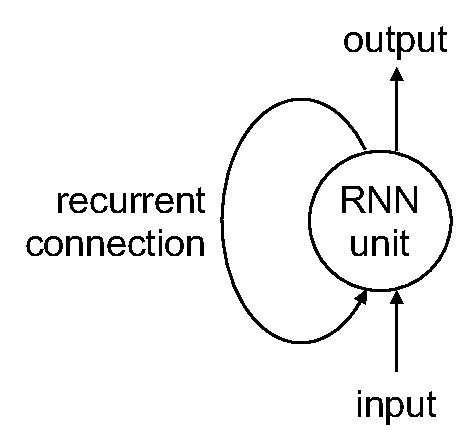
\includegraphics[scale=0.5]{thesis/figures/RNNunit.pdf}
    \caption[Schematic representation of a RNN unit]{Schematic representation of a RNN unit. Adapted from \citet{Chollet:2018}.}
    \label{Fig:RNNunit}
\end{figure}

The cyclical structure of an RNN unit can be unrolled across time (see Figure~\ref{Fig:RNNunfolded}). This illustrates that a RNN is basically a simple neural network that has one layer for each time step that has to be processed per input. This notion of an unfolded RNN also reveals, that a RNN is still trainable through backpropagation. The backpropagation just has to happen across all time steps. This is called backpropagation through time (BPTT) and was introduced by \citet{Werbos:1990}. Theoretically, this feedback structure enables RNN to retain information about sequence elements that have been processed many steps before the current step and use it for the prediction of the current step. However, in practice the vanishing gradient problem occurs\footnote{For more details on the vanishing gradient problem see, e.g., \citet{Bengio:1994}}. This problem makes RNNs basically untrainable for very long sequences.
%
\begin{figure}[htbp]
    \centering
    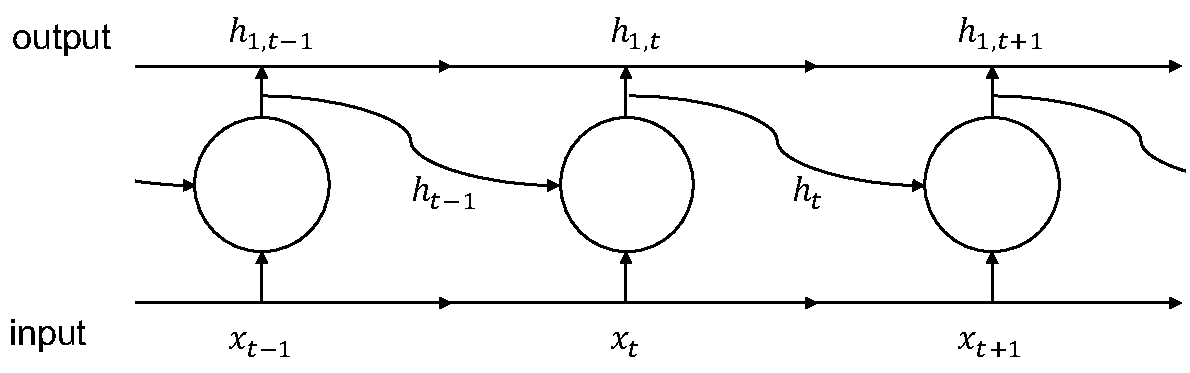
\includegraphics[scale=0.6]{thesis/figures/RNNunfolded.pdf}
    \caption[Schematic representation of an unfolded RNN unit]{Schematic representation of an unfolded RNN unit. Adapted from \citet{Chollet:2018}.}
    \label{Fig:RNNunfolded}
\end{figure}



%%%%%%%%%%%
\subsubsection{Long short-term memory units}

To overcome the vanishing gradient problem, \citet{Hochreiter:1997} developed LSTM units. LSTM units extend RNN units by an additional state. This state can retain information for as long as needed. In which step this additional state is updated and in which state the information it retains is used in the transformation of the input is controlled by three so-called gates\footnote{In their original specification, \citet{Hochreiter:1997} included only two gates. However, as this LSTM specification was still prone to the vanishing gradient problem under some circumstances, \citet{Gers:2000} extended it by a third gate.}. These three gates again have the form of a simple RNN cell. Formally, the gates can be written as (following the notation of \citet{Lipton:2015}\footnote{\cites{Lipton:2015} notation uses $h_{t-1}$ instead of $s_{t-1}$. The notation used here ($s_{t-1}$) accounts for the modern LSTM architecture with peephole connections. For more information see \cite{Gers:2002}.})
%
\begin{equation} \label{Eq:LSTMgates}
\begin{split}
    \vec{i}_t&=\sigma\left(\vec{W}^{(ix)}\vec{x}_t+\vec{W}^{(is)}\vec{s}_{t-1}+\vec{b_i}\right)\\
    \vec{f}_t&=\sigma\left(\vec{W}^{(fx)}\vec{x}_t+\vec{W}^{(fs)}\vec{s}_{t-1}+\vec{b_f}\right)\\
    \vec{o}_t&=\sigma\left(\vec{W}^{(ox)}\vec{x}_t+\vec{W}^{(os)}\vec{s}_{t-1}+\vec{b_o}\right),
\end{split}   
\end{equation}
%
where $\sigma$ is the sigmoid activation function $\sigma(z)=\frac{1}{1+e^{-z}}$, $W$ denotes the weight matrices that are intuitively labeled ($ix$ for the weight matrix of gate $i_t$ multiplied with the input $x_t$ etc.), and $b$ denotes the bias vectors.\footnote{Sometimes, the gates are titled input, output, and forget gate. However, as \citet{Chollet:2018} put it:
\vspace{0.75\dimexpr-\topsep-\partopsep}
\begin{quote}
    ``[T]hese interpretations don’t mean much, because what these [gates] actually do is determined by the contents of the weights parameterizing them; and the weights are learned in an end-to-end fashion [...] making it impossible to credit this or that operation with a specific purpose" (p. 193).
\end{quote}\vspace{\dimexpr-\topsep-\partopsep}
}

Again following the notation of \citet{Lipton:2015}, the full algorithm of a LSTM unit is given by the three gates specified above, the input node
%
\begin{equation} \label{Eq:LSTMinput}
    \vec{g}_t=\sigma\left(\vec{W}^{(gx)}\vec{x}_t+\vec{W}^{(gh)}\vec{h}_{t-1}+\vec{b_g}\right),
\end{equation}
%
the internal state of the LSTM unit at time step $t$
%
\begin{equation} \label{Eq:LSTMstate}
    \vec{s}_t=\vec{g}_t\odot\vec{i}_t+\vec{s}_{t-1}\odot\vec{f}_t,
\end{equation}
%
where $\odot$ is pointwise multiplication, and the output at time step $t$
%
\begin{equation} \label{Eq:LSTMoutput}
    \vec{h}_t=\phi\left(\vec{s}_t\right)\odot\vec{o}_t.
\end{equation}
%
The internal structure of a LSTM cell is further clarified by Figure~\ref{Fig:LSTMunit}. For an intuitive but more detailed explanation of LSTM neural networks see \citet[][Ch. 6.2]{Chollet:2018}.
%
\begin{figure}[htbp]
    \centering
    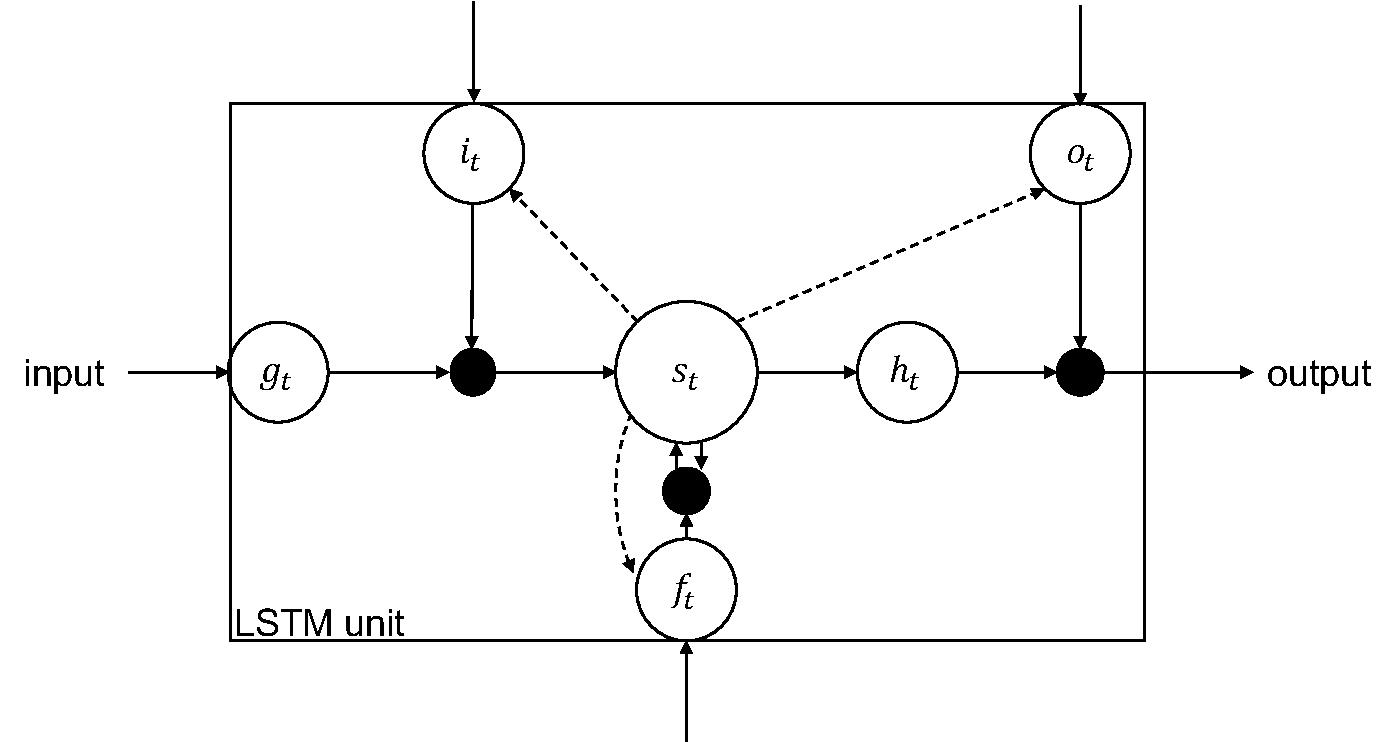
\includegraphics[scale=0.5]{thesis/figures/LSTMunit.pdf}
    \caption[Schematic representation of a LSTM unit]{Schematic representation of a LSTM unit. Adapted from \citet{Graves:2012}. The filled in circles represent the pointwise multiplication operation denoted by $\odot$ in Equation~\ref{Eq:LSTMstate} and~\ref{Eq:LSTMoutput}.}
    \label{Fig:LSTMunit}
\end{figure}

To summarize, all neural networks use the basic building blocks of units that form input, hidden, and output layers. The training process of neural networks involves updating the parameters (weights and biases) of the model based on the gradient descent of a loss function that quantifies the accuracy of a prediction compared to true values. RNN enables the neural network to process individual elements of a sequence or time series sequentially and still use information that was obtained in previous time steps for the current transformation of the input. LSTM RNN is an extension of simple RNN which has the advantage of being able to retain a state over multiple time steps and solves the vanishing gradient problem through the introduction of an additional internal state $\vec{s}_t$. By this, LSTM RNN are capable of learning highly complex, non-linear relationships in time series data which makes them a promising forecasting technique to predict households' very short-term energy consumption and production.



%%%%%%%%%%%
\subsubsection{Implementation of LSTM RNN}

The specific LTSM RNN approach adopted in this study is based on the procedure employed by \citet{Shi:2017} to forecast individual households' energy consumption. However, according to the relevant use case in this study, model training and predictions were performed using only the data of individual households. That means, a LSTM recurring neural network was trained for each household individually using only the households historic consumption patterns and calender features. This differs from \cites{Shi:2017} implementation, that used pooled consumption data of multiple households. Specifically, seven days\footnote{Preliminary results indicated that the autocorrelation in the time series becomes very week in lags beyond one week. Moreover, using the previous week as input data still preserves the weekly seasonality and represents a reasonable compromise between as much input as possible and computational resources needed to process the input in the training process of the LSTM neural network.} of past consumption, an indicator for weekends, and an indicator for Germany-wide holidays were used as input for the neural network in the present study. This follows the one-hot encoding used by \citet{Chen:2018}. The target values were single consumption values in 15-minute aggregation. Take the following example as illustration: The consumption values in 3-minute intervals from 13.11.2017 13:00 until 20.11.2017 13:00 and zero/one-indicators for weekends and holidays (i.e., 3 $\times$ 3,360 data points) are fed into the neural network. The model then produces a single output value that estimates the household's energy consumption in kWh from 20.11.2017 13:00 until 20.11.2017 13:15.

A neural network is defined by several so-called hyperparameters: The number and type of layers, the number of hidden units within each layer, the activation functions used within each unit, dropout rates for the recurrent transformation, and dropout rates for the transformation of the input. These hyperparameters must be chosen specifically for the task at hand and their influence on the model performance is difficult to foresee. For this reason, parameter tuning was employed to find a relatively well working combination of hyperparameter values. Unfortunately, hyperparameter tuning is computationally very resource intensive as for each hyperparameter combination, the model must be fully trained to asses the model performance. Hence, not all possible or sensible combinations of hyperparameters could be assessed. Instead, a random sample of different hyperparameter combinations was chosen and the resulting model configurations trained and evaluated on a randomly chosen data set.

Table~\ref{Tab:LSTMHyperparameters} presents the hyperparameters that were tuned and their respective value ranges. The tuning was done individually for each layer. First layer 1 hyperparameters were tuned. The best found hyperparameter combination was then fixed for layer 1 and the parameters for layer 2 were tuned. This was repeated for layer 3. Optimally, all hyperparameters should be tuned simultaneously. However, due to computational constraints, that was not possible here and, thus, the described, second-best option chosen. As the hyperparameter values specified in Table~\ref{Tab:LSTMHyperparameters} for layer 1 alone result in 81 possible hyperparameter combinations, only samples of these combinations were taken, the resulting models trained and compared. In total, 16 models with one layer, 13 models with two layers and 13 models with 3 layers were tuned. The model tuning was conducted on the Machine Learning (ML) Engine of the Google Cloud Platform. The job was submitted to The ML Engine via Google Cloud SDK and the R package \texttt{cloudml}. The model training was conducted on four Tesla P100 GPUs. The necessary credits to pay for the hardware resources were granted by Google as part of their Google Cloud Platform Free Tier program\footnote{For further details see \url{https://cloud.google.com/free} (last accessed 01.10.2018).}.

\begin{table}[htbp]
    \begin{center}
        {\footnotesize
        \begin{tabular}{l|lcccc}
        \hline \hline
        & \multirow{2}{3em}{hyperparameter} & possible & possible     & sampling & \# of assessed \\
        &                                   & values   & combinations & rate     & combinations   \\
        \hline
                \multirow{4}{3em}{layer 1}  & batch size        & \{128, 64, 32\} & \multirow{4}{1em}{81} & \multirow{4}{1em}{0.2} & \multirow{4}{1em}{16} \\
                                            & hidden units      & \{128, 64, 32\} & & &\\
                                            & recurrent dropout & \{0, 0.2, 0.4\} & & & \\
                                            & dropout           & \{0, 0.2, 0.4\} & & & \\[0.2cm]
                                            & hidden units      & \{128, 64, 32\} & & & \\
                layer 2                     & recurrent dropout & \{0, 0.2, 0.4\} & 26 & 0.5 & 13 \\
                                            & dropout           & \{0, 0.2, 0.4\} & \\[0.2cm]
                                            & hidden units      & \{128, 64, 32\} & \\
                layer 3                     & recurrent dropout & \{0, 0.2, 0.4\} & 26 & 0.5 & 13 \\
                                            & dropout           & \{0, 0.2, 0.4\} & \\
            \hline \hline
        \end{tabular}}
    \end{center}
    \caption[Hyperparameters tuned for optimal LSTM RNN model specification]{The hyperparameters and their possible values that were tuned for an optimal LSTM RNN model specification.}
    \label{Tab:LSTMHyperparameters}
\end{table}

As it turned out, a deeper model architecture of multiple layers did not increase the model performance enough to justify the greatly increased computing time for model training introduced by the much higher number of model parameters that would have to be trained\footnote{A one layer, 32 hidden units LSTM RNN with one output unit has 4,641 trainable parameters while a two layer, 32 hidden units each LSTM RNN with one output unit has already 12,961 trainable parameters.}. Therefore, a model of the following specification was used for the prediction of a single energy consumption value for the next 15 minutes:

\begin{multicols}{2}
    \indent\textit{layers: $1$\\
    \indent hidden units: $32$\\
    \indent dropout rate: $0$\\
    \indent recurrent dropout rate: $0$\\
    \indent batch size: $32$\\
    \indent number of input data points: $3,360$\\
    \indent number of training samples\footnote{Each sample consists of an array of the dimensions batch size $\times$ input data points $\times$ input features, i.e., 32$\times$3,360$\times$3. Thus, the number of training samples has to be multiplied by the batch size and the number of data points that are aggregated for each prediction (i.e., 5) to get the total length of data points covered in the training process: $700\times32\times5=112000$ data points. This is equivalent to the time period from 01.01.2017 00:00 to 2017-08-22 09:03}: $700$ \\
    \indent number of validation samples: $96$}
\end{multicols}


The general procedure of model training, model assessment and prediction generation is shown in Procedure~\ref{Alg:LSTMimplementation}. The parameter tuple is set globally for all household data sets based on the hyperparameter tuning. Thereafter, the same procedure is repeated for each data set.

First, the consumption data time series is loaded, target values are generated, and the input data is transformed. The transformation consists of normalizing the log-values of the consumption per 3-minute interval between 0 an 1. This ensures fast convergence of the model training process. Appendix~\hyperlink{AppA3:Figures:transform}{A3} exemplary shows the distribution of energy consumption for consumer 020 before and after the transformation.  The data batches for the model training and the cross-validation are served to the training algorithm by so-called generator functions. The generator functions are called by the training algorithm and supply samples of data from the input time series infinitely. The number of training and validation steps that are necessary for the model to see the complete input time series is controlled by the training algorithm.
%
\begin{algorithm}[htbp]
\floatname{algorithm}{Procedure}
\caption{Supervised learning of LSTM neural network and prediction.}\label{Alg:LSTMimplementation}

\begin{algorithmic}[1]
\State{Set parameter tuple $<l, u, b, d>$: number of layers $l \subseteq L$, number of hidden LSTM-units $u \subseteq U$, batch size $b \subseteq B$, and dropout rate $d \subseteq D$.}
\State{Initiate prediction matrix $P$ and list for error measures $\Theta$.}
\For{Household $i$ in data set pool $I$}
    \State{Load data set $\Psi_i$.}
    \State{Generate target values $\vec{y}$ by aggregating data to 15-min intervals.}
    \State{Transform time series in data set $\Psi_i$ and add calender features.}
    \State{Set up training and validation data generators according to parameter tuple $<b, d>$.}
    \State{Split data set $\Psi_i$ into training data set $\Psi_{i,tr}$ and testing data set $\Psi_{i,ts}$.}
    \State{Build LSTM RNN $\zeta_i$ on Tensorflow with network size $(l, h)$.}
    \Repeat
    \indent\State{\textbf{At} $k^{th}$ epoch \textbf{do}:}
        \State{\multiline{%
        Train LSTM RNN $\zeta_i$ with data batches $\varphi_{train} \subseteq \Psi_{i,tr}$ supplied by training data generator.}}
        \State{\multiline{%
        Evaluate performance with mean absolute error $\Lambda_k$ on cross-validation data batches $\varphi_{val} \subseteq \Psi_{i,tr}$ supplied by validation data generator.}}
    \Until{$\Lambda_{k-1}-\Lambda_{k}<0.001$ for the last 3 epochs.}
    \State{Save trained LSTM RNN $\zeta_i$.}
    \State{Set up testing data generator according to tuple $<b, d>$.}
    \State{\multiline{%
    Generate predictions $\vec{\widehat{y}_i}$ with batches $\varphi_{ts} \subseteq \Psi_{i,ts}$ fed by testing data generator into LSTM RNN $\zeta_i$.}}
    \State{Calculate error measures $\Theta_i$ to assess performance of $X_i$.}
    \State{Write prediction vector $\vec{\widehat{y}_i}$ into column $i$ of matrix $P$.}
\EndFor.
\State{Save matrix $P$.}
\State{\textbf{End.}}
\end{algorithmic}

\end{algorithm}
%

Second, the LSTM RNN is compiled and trained with Keras which is a neural network API written in Python. It can employ several machine learning back-ends that are based on computational graphs. The most commonly known and very well-developed back-end is TensorFlow by Google which is an open source software that enables parallel GPU-based numerical computations\footnote{For more details on tensors and TensorFlow see \citet{Abadi:2017} and \citet{Goldsborough:2016}.}. The \texttt{keras} R package (v2.2.0.9) is a wrapper of the Python library and is maintained by \citet{chollet:2017kerasR}. The package was used with RStudio v1.1.453 and TensorFlow 1.11.0 as back-end. The model training and prediction for each household was performed on a Windows Server 2012 with 12 cores and 24 logical processors of Intel Xeon 3.4 GHz CPUs\footnote{The computing resources were kindly provided by the Humboldt Lab for Empirical and Quantitative Research (LEQR) at the School of Business and Economics, Humboldt-University Berlin.}. The model training is done in a differing number of epochs as early stopping was employed. That means, once the mean absolute error on the validation data did not decrease by more than 0.001 in three consecutive epochs, the training process is stopped (see line 14 in Procedure~\ref{Alg:LSTMimplementation}). Early stopping is a common and well-suited approach to prevent overfitting \citep{Chollet:2018}.

Finally, the trained model is used to generate predictions on the test set that comprises data from 01.10.2017 00:00 to 01.01.2018 00:00 (i.e., 44,180 data points). As the prediction is made in 15-minute intervals, in total, 8,836 data points are predicted. Using the error measures described in Section~\ref{Sec:Method;Subsec:Error}, the model performance is assessed. Additionally, the predictions for all data sets are saved for the evaluation in the market mechanism implemented in a smart contract by \citet{Mengelkamp:2018a}.

%%%%%%%%%%%%%%%%%
%%%   LASSO   %%%
%%%%%%%%%%%%%%%%%

\subsection{Statistical method based forecasting approach} \label{Sec:Method;Subsec:LASSO}

To complement the machine learning approach of LSTM neural networks with a statistical approach, a second, regression-based method was chosen. For this purpose, the sparse autoregressive LASSO algorithm proposed by \citet{Li:2017} seemed most suitable. Statistical methods have the advantage of much lower model complexity compared to neural networks which makes them computationally much less resource intensive. Additionally, a LASSO-based approach as employed by \citet{Li:2017} maintains the easy interpretability of linear methods.



%%%%%%%%%%%
\subsubsection{Sparse autoregressive LASSO}

The approach proposed by \citet{Li:2017} is based on the linear autoregressive model
%
\begin{equation} \label{Eq:ARmodel}
    y_{t+1}=\beta_0+\sum_{i=0}^I\beta_iy_{t-i}+\varepsilon_t,
\end{equation}
%
where the future demand $y_{t+1}$ depends linearly only on historical data $y_{t-i}$ plus a random Gaussian noise $\varepsilon_t$, with $\beta_i$ being the coefficient for lag-order $i$. In the following, vector $\left[y_t, y_{t-1}, \dots, y_{t-I}\right]^T$ is written as $\vec{x_t}$. To be able to use the model in Equation~\ref{Eq:ARmodel} to make predictions, the vector $\widehat{\beta}$ has to be estimated such that the sum of squared errors is minimal. However, as the OLS estimator
%
\begin{equation} \label{Eq:betaOLS}
    \widehat{\vec{\beta}}_{\text{OLS}}=\argmin_{\vec{\beta}}\left\lVert(\vec{y}-\vec{X}\vec{\beta}\right\rVert^2_2
\end{equation}
%
minimizes the sum of squared error within the data used to estimate $\widehat{\vec{\beta}}_{\text{OLS}}$, it is very likely to overfit the data and to have a very poor prediction accuracy on new data.

This risk of model overfitting can be mitigated by including only lag-orders of the historical data that are relevant for the estimation of $y_{t+1}$ and, thereby, reducing the number of regressors. Thus, \citet{Li:2017} use LASSO \citetext{least absolute shrinkage and selection operator, \citet{Tibshirani:1996}} to find a sparse autoregressive model which generalizes better to new data. Formally, the LASSO estimator can be written as
%
\begin{equation} \label{Eq:betaLASSO}
    \widehat{\vec{\beta}}_{\text{LASSO}}=\argmin_{\vec{\beta}}\frac{1}{2}\left\lVert(\vec{y}-\vec{X}\vec{\beta}\right\rVert^2_2+\lambda\left\lVert\vec{\beta}\right\rVert_1,
\end{equation}
%
where $\lambda$ is a parameter that controls the level of sparsity in the model, i.e., the number of lag-orders that are included to predict $y_{t+1}$. This model specification selects the best recurrent pattern in the energy time series by shrinking coefficients of irrelevant lag-orders to zero and, thereby, improves the generalizability of the prediction model.



%%%%%%%%%%%
\subsubsection{Implementation of sparse autoregressive LASSO}

The sparse autoregressive LASSO approach was implemented using the R package \texttt{glmnet} \citep{Friedman:2010}. Again, as for the LSTM RNN approach, model training and prediction were performed for every household individually. Following \cites{Li:2017} procedure, only historical consumption values were used as predictors. Specifically, for comparability to the LSTM approach seven days of lagged consumption values served as input to the LASSO model. The response vector consisted of single consumption values in 15-minute aggregation. The same example as above is presented for illustration of the prediction task: The consumption values in 3-minute intervals from 13.11.2017 13:00 until 20.11.2017 13:00 (i.e., 3,360 data points) are available to the model for prediction. 
Based on the training data, the model chooses the lagged values with the highest predictive power and makes a linear estimation of a single value for the household's energy consumption in kWh from 20.11.2017 13:00 until 20.11.2017 13:15.

The \texttt{glmnet} package used fits a generalized linear model with the  elastic-net penalty
%
\begin{equation} \label{Eq:elasticnetpenalty}
    \lambda\left[(1-\alpha)\left\lVert\vec{\beta}\right\rVert^2_2/2 + \alpha \left\lVert\vec{\beta}\right\rVert_1\right],
\end{equation}
%
where $\alpha=1$ to perform LASSO. Hence, the penalty term here is $\lambda\left\lVert\vec{\beta}\right\rVert_1$. The parameter $\lambda$ has to be tuned. This can be done using the package's cross-validation function with parallel computing. As a linear autoregressive model had to be fitted, the Gaussian family option of the package was chosen. The objective function of the Gaussian family LASSO model is
%
\begin{equation} \label{Eq:glmnetobjfun}
    \min_{(\beta_0, \vec{\beta)}}\frac{1}{2N} \sum_{i=1}^N (y_i -\beta_0-x_i^T\vec{\beta})^2+\lambda\left\lVert\vec{\beta}\right\rVert_1,
\end{equation}
%
where $\lambda \geq 0$ is the tuning parameter that controls the penalization of the number of coefficients. The objective function is solved by applying coordinate descent \citep[see][]{Friedman:2010}.

As the LASSO model requires a predictor matrix, the time series of each household is split in sequences of length $n=3,360$ with 5 data points skipped in between. The skip accounts for the fact, that the response vector is comprised of 15-minute interval consumption values (i.e., five 3-minute consumption values). The detailed description of the model estimation and prediction is presented in Procedure~\ref{Alg:LASSOimplementation}.
%
\begin{algorithm}[htbp]
\floatname{algorithm}{Procedure}
\caption{Cross-validated selection of $\lambda$ for LASSO and prediction.} \label{Alg:LASSOimplementation}

\begin{algorithmic}[1]
\State{Initiate prediction matrix $P$ and list for error measures $\Theta$.}
\For{Household $i$ in data set pool $I$}
    \State{Load data set $\Psi_i$.}
    \State{Generate target values $\vec{y}$ by aggregating data to 15-min intervals.}
    \State{Split data set $\Psi_i$ into training data set $\Psi_{i,tr}$ and testing data set $\Psi_{i,ts}$.}
    \State{Generate predictor matrix $M_{tr}$ by slicing time series $\Psi_{i,tr}$ with sliding window.}
    \State{Generate sequence of $\lambda$-values $\{l_s\}_{s=1}^L$.}
    \State{Set number of cross-validation (CV) folds $K$.}
    \State{Split predictor matrix $M_{tr}$ into $K$ folds.}
    \For{$k$ in $K$}
        \State{Select fold $k$ as CV testing set and folds $j\neq k$ as CV training set.}
        \For{each $l_s$ in $\{l_s\}_{s=1}^L$}
            \State{Compute vector $\widehat{\vec{\beta}}_{k,l_s}$ on CV training set.}
            \State{Compute mean absolute error $\Lambda_{k,l_s}$ on CV testing set.}
        \EndFor.
    \EndFor.
    \State{For each $\widehat{\vec{\beta}}_{k,l_s}$ calculate average mean absolute error $\bar{\Lambda}_s$ across the $K$ folds.}
    \State{\multiline{%
    Select cross-validated $\lambda$-value $l_s^{CV}$ with the highest regularization (i.e., lowest number of non-zero $\beta$-coefficients) within one standard deviation of the minimum $\bar{\Lambda}_s$.}}
    \State{Compute $\widehat{\vec{\beta}}_{l_s^{CV}}$ on complete predictor matrix $M_{tr}$.}
    \State{Generate predictor matrix $M_{ts}$ by slicing time series $\Psi_{i,ts}$ with sliding window.}
    \State{Generate predictions $\vec{\widehat{y}_i}$ from predictor matrix $M_{ts}$ and coefficients $\widehat{\vec{\beta}}_{l_s^{CV}}$.}
    \State{Calculate error measures $\Theta_i$ to assess performance.}
    \State{Write prediction vector $\vec{\widehat{y}_i}$ into column $i$ of matrix $P$.}
\EndFor.
\State{Save matrix $P$.}
\State{\textbf{End.}}
\end{algorithmic}

\end{algorithm}
%

After generating the predictor matrix for the model estimation, the optimal $\lambda$ is found in a K-fold cross-validation. Here, $K$ is set to 10. The sequence of $\lambda$-values that is tested in the cross-validation is by default of length $L=100$. However, the \texttt{glmnet} algorithm uses early-stopping to reduce computing times if the percent of null deviance explained by the model with a certain $\lambda$ does not change sufficiently from one to the next $\lambda$-value. According to \citet{Friedman:2010} the sequence of $\lambda$-values is constructed by calculating the minimum lambda value as a fraction of the maximum lambda value ($\lambda_{min}=\varepsilon\lambda_{max}$, where $\lambda_{max}$ is such that all $\beta$-coefficients are set equal to zero) and moving along the log-scale from $\lambda_{max}$ to $\lambda_{min}$ in $L$ steps. The cross-validation procedure identifies the biggest $\lambda$ that is still within one standard deviation of the $\lambda$ with the lowest mean absolute error. The final coefficients for each household are then computed by solving Equation~\ref{Eq:betaLASSO} for the complete predictor matrix.

Thereafter, the predictions are made on the testing data. For this, again, the time series is sliced according to the sliding window of length $n=3,360$ skipping 5 data points and written into a predictor matrix. This matrix comprises data from 01.10.2017 00:00 to 01.01.2018 00:00 (i.e., 8,836 cases of 3,360 lagged values), resulting again in 8,836 predicted values as in the case of the LSTM approach described above. The predictions on all data sets were assessed using the error measures described in Section~\ref{Sec:Method;Subsec:Error} and saved for the evaluation of the prediction in the context of the market mechanism implemented in a smart contract by \citet{Mengelkamp:2018a}.


%%%%%%%%%%%%%%%%%%%%%%%%%%
%%%   Error measures   %%%
%%%%%%%%%%%%%%%%%%%%%%%%%%

\subsection{Error measures} \label{Sec:Method;Subsec:Error}

Error measures play an essential role in any prediction task. Also called performance metrics, these measures are used to quantify the accuracy of the prediction generated by a forecasting model \citep{zor:2017}. Without assessing the prediction accuracy through error measures, it is impossible to quantify whether the proposed forecasting technique is an improvement compared to the benchmark models \citep{Meer:2018}. Moreover, error measures are used by supervised machine learning algorithms to assess the prediction accuracy and to accordingly adjust their parameters.

However, there is a wide variaty of error measures available and actively used in the research of energy forecasting. \citet{zor:2017} reviewed the energy forecasting literature published in 2017 and found eight different error measures that were used to assess the forecasting accuracy. Among those, mean absolute percentage error was used in 83~\% of the studies, with mean absolute error and root mean squared error coming third and second with 32~\% and 31~\% respectively. As these results suggest, there is a lack of standardization in the field of energy forecasting regarding the usage of the various available error measures \citep[see also][]{Meer:2018}. This is aggravated by the fact, that different error measures are appropriate in different use cases and cannot be generally applied without careful consideration. Therefore, the following section introduces the error measures used in the research at hand and discusses their advantages and disadvantages. Following the suggestion of \citet{Hoff:2013} several performance metrics will be used to evaluate the quality of the forecast models. The choice of performance metrics is mostly guided by the compilation provided by \citet{Meer:2018}.


%%%%%%%%%%%
\subsubsection{MAE and RMSE}

Error measures can be classified into representing absolute or percentage errors \citep{Hoff:2013}. Absolute error measures, for example, are mean absolute error (MAE) and root mean squared error (RMSE). Both are quite popular as performance metrics for energy forecasts \citep{zor:2017}. Absolute error measures can be formulated in terms of a vector function 
%
\begin{equation} \label{Eq:vectorfunction}
    E=F\left(\vec{f}, \vec{x}\right),
\end{equation}

\noindent where $\vec{f}$ and $\vec{x}$ are the forecasted and actual data vectors respectively \citep{Haben:2014}. The metric $F$ is then the absolute p-norm,
%
\begin{equation} \label{Eq:pnorm}
    E_p=\left\lVert\vec{f}-\vec{x}\right\rVert_p=\biggl(\sum_{t=1}^N \left|f_t-x_t\right|^p\biggr)^{1/p},
\end{equation}

\noindent for $p\geq1$ \citep[][p. 52]{golub:2012}. The MAE belongs to this type of error and is defined as the average of the absolute differences between the predicted and true values \citep{Hoff:2013}:
%
\begin{equation} \label{Eq:MAE}
\text{MAE}=\frac{1}{N}\sum_{t=1}^N\left|\widehat{x}_t-x_t\right|,    
\end{equation}

\noindent where N is the length of the forecasted time series, $\widehat{x}_t$ the forecasted value and $x_t$ the observed value. This is equivalent to Equation~\ref{Eq:pnorm} with $p=1$. Similar to the MAE and also of the p-norm type of error measure is the RMSE. Instead of summing up the \textit{absolute} differences, the RMSE is defined as the square root of the average \textit{squared} differences (which is equivalent to $p=2$ in Equation~\ref{Eq:pnorm}):
%
\begin{equation} \label{Eq:RMSE}
\text{RMSE}=\sqrt{\frac{1}{N}\sum_{t=1}^N\left(\widehat{x}_t-x_t\right)^2}.
\end{equation}

\noindent RMSE, thus, puts more weight on large deviations between forecast and observation than MAE \citep{Meer:2018}. Therefore, RMSE is more suitable in the presence of a lot of noise, as it does not mask a small amount of large errors in the presence of a majority of small errors as the MAE does \citep{Zhang:2015}. One disadvantage of these measures is that they are not scale independent. This makes them unsuitable to compare the prediction accuracy of a forecasting model on different time series. However, they are suitable as loss function in machine learning algorithms and for the comparison of sophisticated forecasting techniques with benchmark models on the same time series. Moreover, they do not rely on denominator-related assumptions -- as percentage error measures do -- which makes them more robust \citep{Hoff:2013}.


%%%%%%%%%%%
\subsubsection{MAPE and NRMSE}

Even though MAE and RMSE are widely used, they are not useful to compare the forecast accuracy across different time series as they are not scale independent \citep{Meer:2018}. Therefore, it is reasonable to complement them with percentage error measures which are normalized by a denominator. However, depending on the application, there may be several denominators that could be used, each coming with certain advantages and disadvantages. \citet{Hoff:2013}, for example, found that the choice of the denominator influences the calculated error results of solar irradiance forecasts substantially. Generally, the denominator may fall into one of two categories: (1) It is a fixed single number that is representative of the time series to be forecasted (e.g., the maximum value of the time series, the average value of the time series or the maximum capacity of the electrical system under consideration) as proposed by \citet{Hoff:2013} and agreed on by \citet{Meer:2018}. (2) The denominator can be different for every pair of true and predicted value (i.e., the true value is used as denominator for each pair of true and predicted values) as defined by \citet{Hyndman:2006} and used by \citet{xie:2018}, for example. 

Investigating forecasting error measures for PV power plants, \citet{Hoff:2013} conclude that normalizing the MAE by the average output of a PV power plant is most desirable to compute the MAPE. However, as \citet{Meer:2018} did not find any literature supporting this for consumption forecasting, the MAPE and NRMSE normalised by the true value will be used here. Hence, they are defined as
%
\begin{equation} \label{Eq:MAPE}
\text{MAPE}=\frac{100}{N}\sum_{t=1}^N\left|\frac{\widehat{x}_t-x_t}{x_t}\right|,
\end{equation}
and
\begin{equation} \label{Eq:NRMSE}
\text{NRMSE}=\sqrt{\frac{100}{N}\sum_{t=1}^N\left(\frac{\widehat{x}_t-x_t}{x_t}\right)^2}.
\end{equation}

\noindent However, as \citet{Hyndman:2006} point out, this choice of denominator is problematic in the presence of zero values, as the fraction $\frac{\widehat{x}_i-x_i}{\bar{x}_t}$ is not defined for $x_t=0$. Therefore, time series containing zero values cannot be assessed with this definition of the MAPE and NRSME. This has to be kept in mind for the further analysis. Furthermore, it is important to recognize that percentage errors assume a meaningful zero value (which is not the case for, e.g., temperature scales like Fahrenheit or Celsuis) \citep{Hyndman:2006}. However, as kWh as measurement unit of the time series used here does have a meaningful zero value, that is of no concern in this study. Again, just as RMSE relative to MAE, NRSME is more sensitive to outliers than MAPE.


%%%%%%%%%%%
\subsubsection{Further error measures}

To overcome the shortage of an undefined fraction in the presence of zero values that MAPE and NRMSE suffer from, the mean absolute scaled error (MASE) was proposed by \citet{Hyndman:2006}. According to them, MASE is applicable even if the time series includes a great number of zero values (e.g., night-time PV energy production) and, as further advantage, MASE does not put a heavier penalty on positive errors as MAPE does. To compute MASE, the MAE is normalized with the in-sample mean absolute error of the persistence model forecast \citet{Hyndman:2006}:
%
\begin{equation} \label{Eq:MASE}
\text{MASE}=\frac{\text{MAE}}{\frac{1}{n-1}\sum_{t=2}^N\left|x_t-x_{t-1}\right|}.
\end{equation}

Unfortunately, all metrics described above can be misleading in the presence of sudden, large fluctuations. \citet{Vallance:2017} show, that forecasts that follow the observed time series more closely but with a small temporal mismatch (e.g., sudden fluctuation is forecasted but with a delay) may have the same or worse RMSE values than a smooth forecast ignoring sudden fluctuations but follow the trend of the observed time series well. A similar case is put forward by \citet{Haben:2014}. To address this issue, several new metrics have been proposed recently that take into account the ability of the forecast to predict sudden fluctuation in the time series, also called ramp events \citep{Zhang:2015}. As the energy consumption of households is also characterized by large and sudden fluctuation, this might be of concern for the forecasting task at hand as well.

A proposed metric that captures the ability of a forecasting technique to accurately follow such ramp events is the ramp metric \citep{Vallance:2017} which is based on an application of the swinging door algorithm by \citet{Florita:2013}. Closely connected to the notion of detecting ramp events but with a focus on the temporal aspect of the forecast, \citet{Haben:2014} propose an adjusted p-norm based error metric, that allows for permutation of the observed time series in a specified interval to find the permutation that translates to the lowest absolute error. Thereby, the requirement of temporal accuracy of the forecast is relaxed and the error is smaller as long as a fluctuation is predicted correctly, even if the timing is slightly incorrect. Thereby, the double penalty of the standard absolute error measures (such as MAE and RMSE) is avoided \citep{Haben:2014}.

However, the prediction task at hand aims to forecast just one value ahead. Therefore, solely the error for each predicted time step individually is of interest here. In this setting, a prediction that is correct in magnitude but not correct in timing is not preferable to an equally incorrect prediction at every point in time. This is due to the fact, that the prediction is not used to plan actions for an extended period of multiple time point (as is often the case for solar or wind generation forecasts) but just serves as a basis for a single bid at a single point in time, which does not take into account potential future developments of a household's energy consumption or production. Thus, the ramp score and adjusted absolute error metrics briefly presented above -- even though highly relevant to the field of energy forecasting as a whole -- will not be used in the research at hand. Analogically, the sometimes recommended Kolmogorov-Smirnov Integral (KSI) \citep{Espinar:2009} is not used here, as it describes the similarity of the forecasted and observed time series' probability distributions and not the accuracy of point predictions.



%%%%%%%%%%%%%%%%%%%%%%%%%%%%%
%%%   Market simulation   %%%
%%%%%%%%%%%%%%%%%%%%%%%%%%%%%

\subsection{Market simulation} \label{Sec:Method;Subsec:Market}

The market mechanism used to evaluate the prediction performance in a simulated blockchain-based local energy market is based on \cites{Mengelkamp:2018a} developed smart contract architecture. They use a market mechanism with discrete closing times every 15 minutes. Each consumer and each prosumer submit one order per interval. Their asks and bids are matched in a closed double auction that yields a single equilibrium price per interval. In their setup, the market mechanism is implemented as a smart contract for the Ethereum-blockchain and coded in Solidity\footnote{Solidity is a high-level programming language with a syntax similar to JavaScript that is specifically designed to write smart contracts for the Ethereum blockchain \citetext{see \citet{Ethereum:2018doc} for details}}. Their smart contract is deployed on a private blockchain\footnote{The code for the implementation of the private blockchain and the smart contract was not publicly available at the time of writing. The author, however, had access and used the smart contract Solidity code as basis for the market simulation.}.

This study replicated the Solidity-based market mechanism for simulation purposes in R. Contrary to \citet{Mengelkamp:2018a}, the focus of this study is not the proof-of-concept, that a smart contract-based market mechanism on a blockchain can serve a local energy market. Hence, the Solidity coded market mechanism used by \citet{Mengelkamp:2018a} is not suitable to simulate the market outcomes depending on the forecasting accuracy. Recreating the market mechanism in R instead allows for a much more flexible and time-efficient analysis of the market outcomes with and without prediction errors.

The simulation of the market mechanism follows five major steps: First, the consumption and production values of each market participant per 15-minute interval from 01-10-2017 00:00 to 01.01.2018 00:00 are retrieved. These values are either the true values as yielded by the aggregation of the raw data or the prediction values as estimated by the best performing prediction model. Second, for each market participant a zero-intelligence limit price is generated. That is, the prices are drawn randomly from the uniform distribution $\textit{U}\{12.31,24.69\}$. The lower bound is the German feed-in tariff of 12.31 $\frac{\text{EURct}}{\text{kWh}}$ and the upper bound is -- for consistency with \citet{Mengelkamp:2018a} -- the the average German electricity price in 2016 of 28.69 $\frac{\text{EURct}}{\text{kWh}}$ \citep{Heidjann:2017}. This agent behavior has been shown to generate efficient market outcomes in double auctions \citep{Gode:1993} and is rational in so far as electricity sellers would not accept a price below the feed-in tariff and electricity buyers would not pay more than the energy utility's price per kWh. However, this assumes that the agents do not consider any non-price related preferences, such as strongly preferring local renewable energy \citep{Mengelkamp:2018a}. Third, for each trading slot (i.e., every 15-minute interval) the bids and asks are ordered in price-time precedence. Given the total supply is lower than the total demand, the lowest bid price that can still be served determines the equilibrium price. Given the total supply is higher than the total demand, the overall lowest bid price determines the equilibrium price. In the case of over- or undersupply, the residual amounts are traded at the feed-in (12.31 $\frac{\text{EURct}}{\text{kWh}}$) or the regular household consumer electricity tariff (28.69 $\frac{\text{EURct}}{\text{kWh}}$) with the energy utility. Fourth, the applicable price for each bid and ask are determined and the settlement amounts, resulting from this price and the energy amount ordered, are calculated. In the case of using predicted values for the bids, there is an additional fifth step. After the next trading period, when the actual energy readings are known, any deviations between predictions and true values are settled with the energy utility using the feed-in or household consumer electricity tariff. This leads to correction amounts that are deducted or added to the original settlement amounts. For the market simulation perfect grid efficiency and, hence, no transmission losses are assumed \citep{Mengelkamp:2017:Trading}.

This procedure results in two prices per trading slot that can be analyzed: The equilibrium price and the weighted average of the equilibrium price and the utility's tariff. Moreover, the cost for each consumer per trading slot, the revenue for each producer per trading slot and the over- or undersupply per interval are recorded. These measures were analyzed using summary statistics and graphical means for varying amounts of the total energy production within the LEM.



%%%%%%%%%%%%%%%%%%%%%%%%%%%%%%%%%%%%%%%%%%%%%%%%%%%%%%%%%%%%%%%%%


\section{Data}\label{Sec:Data}



%%%%%%%%%%%%%%%%%%%%%%%
%%%   Data source   %%%
%%%%%%%%%%%%%%%%%%%%%%%

\subsection{Source}\label{Sec:Data;Subsec:Source}

The data used for the present research was provided by Discovergy GmbH.\footnote{The data can be downloaded from \url{https://research.discovergy.com}.} Discovergy installs and maintains smart meters in German households for a one-time installation and monthly maintenance fee. Customers in return get various services centered around the analysis and visualization of their energy consumption and/or production. Discovergy describes itself as a full-range supplier of smart metering solutions offering transparent energy consumption and production data for private and commercial clients \citep{Discovergy:2018}. All energy measurements of their Discovergy smart meters can be accessed by customers through a web portal and mobile app. Additionally, various services are offered, such as, tips for energy savings potential, irregular consumption pattern warnings, personal energy reporting, and consumption analysis of individual appliances.

To be able to offer such data-driven services, Discovergy smart meters\footnote{Discovergy currently installs for private household clients the EasyMeter Q3D standard load profile meter which is connected to the Discovergy Meteorit TM smart meter gateway which records and transmits the recordings to Discovergy servers. The meter specifications can be found here: \texttt{https://discovergy.com/files/sources/product-information/SLP\_Zaehler.pdf} (in German).} record energy consumption and production near real-time -- i.e., 2-second intervals -- and send the readings to Discovergy's servers for storage and analysis. Therefore, Discovergy has extremely high resolution energy data of their customers at their disposal. This high resolution is in stark contrast to the half-hourly or even hourly recorded data used in previous studies \citep[e.g.,][]{Arora:2016,Auder:2018,Shi:2017,Gerossier:2017}.

To the authors knowledge, there is no research using Discovergy smart meter data, apart from \citet{Teixeira:2017} that used the data as simulation input but not for analysis or prediction. As Discovergy never provided data for external research purposes before, there was no suitable process to retrieve the data from their internal data storage solutions available. For this reason, the author had to provide an API client for the Discovergy REST API to export data from pre-selected meters.



%%%%%%%%%%%%%%%%%%%%%%
%%%   Obtainment   %%%
%%%%%%%%%%%%%%%%%%%%%%

\subsection{Obtainment}\label{Sec:Data;Subsec:Obtainment}

As all Discovergy smart meters send their measurements in real-time to servers for storage, visualization and analysis, customers can access their meters and measurements through a web application and app. Additionally, customers with the need for automated data access can interact with the stored meter measurements through predefined endpoints. These endpoints serve as an application programming interface (API) called Discovergy REST API \citep{DiscovergyAPI:2018}. By providing the credentials for their Discovergy account\footnote{Sign up for a Discovergy account is open to everyone at \url{https://my.discovergy.com/login}. The account provides access to the Discovergy API for developers, without the need of being a Discovergy customer. However, only customers with an installed Discovergy smart meter, that is associated with their account, will have access to actual smart meter data. For testing purposes though, the Discovergy customer service can associate dummy meters as the one used for the demo web portal (\url{http://my.discovergy.com/demo}) with any account.}, developers can send requests to a specified endpoint URL. The API returns to such a request a data object formatted in JavaScript Object Notation (JSON). For example, a user authenticates herself with her account credentials and requests the endpoint \texttt{/meters} with the verb \texttt{GET} at the base URL \url{https://api.discovergy.com/public/v1}. In response, the server returns a JSON object containing all meter IDs the user has access to.

To automate the process of data retrieval from the Discovergy servers, the author of this study had to program an API client, which had to be compliant with the constraints of a RESTful architecture\footnote{REST refers to Representational State Transfer and describes an architetural style that ensures interoperability of systems through the web \citep[][Ch. 5]{fielding:2000}.}. This client had to be able to authenticate the user with account credentials provided in a flat file, request the readings for one year in 3-minute intervals of all meters specified in another flat file, and export the returned JSON data to a specified path. As the API had restrictions on the maximum time span of readings that could be returned depending on the measurement resolution (i.e., returns at most 10 days in 3-minute resolution), the client had to to make 37 request per meter to cover the whole year of 2017 in 10 day periods. As mentioned above, the measurement resolution of the Discovergy smart meters is with 2-second intervals much higher than the 3-minute intervals requested. However, the data management system employed by Discovergy already provides 3-minute aggregations of the original recordings which can be retrieved by specifying the according parameter in the API client.

The client was developed in Java based on the demo client provided in the Discovergy REST API documentation \citep{DiscovergyAPI:2018}. The code of the customized API client can be found in Appendix~\hyperlink{AppC1:Code:API}{C1}. After development, the client was sent to an Discovergy employee who used an administrative account with access to a sufficiently large number of smart meters to retrieve the data sets used in this study. Unfortunately, it is not known to the author what selection criteria, other than having complete data for all of 2017, were used by Discovergy internally to chose the meters of which the data was provided. Therefore, it is not possible to evaluate how representative the provided data is regarding Discovergy customers or even energy consuming/producing households in general. After retrieving the data, Discovergy converted the data to csv-files. To facilitate the file transfer, the resulting files were made available for download on a dedicated web domain and, by the time of writing, are available to the general public here: \url{https://research.discovergy.com} (last accessed on 31.10.2018). 



%%%%%%%%%%%%%%%%%%%%%%%%%%%%
%%%   Data description   %%%
%%%%%%%%%%%%%%%%%%%%%%%%%%%%

\subsection{Description}\label{Sec:Data;Subsec:Description}

The data comes in 200 individual csv-files each containing the meter readings of a single smart meter. The readings are recorded in 3-minute intervals and range from 01.01.2017 00:00:00 to 01.01.2018 00:00:00. This translates into 175,201 observations per smart meter. Each smart meter measures energy consumption, energy production and power over all phases installed in the meter and records them together with a timestamp in Unix milliseconds. For this research, only energy consumption and production are relevant. In summary, the data used here are 200 individual data sets each containing two time series (energy consumption and energy production) with 175,201 observations evenly spaced in 3-minute intervals.

In Table~\ref{Tab:c056} and \ref{Tab:p089}, preprocessed and correctly formatted samples of the data for consumer 56 and prosumer 89 containing 6 measurement points are shown.
%
\begin{table}[htbp]
    \csvreader[centered tabular=c|cc,
    table head=
    \hline\hline
    \textbf{time} & \textbf{energy} & \textbf{energyOut} \\
    \hline
    \ldots & \ldots & \ldots \\,
    head to column names,
    separator=comma,
    respect all,
    late after line=\\,
    table foot=
    \ldots &  \ldots & \ldots \\\hline\hline]
    {tables/consumer-00000056_glimpse.csv}{}%
    {\csvcolii & \csvcoliii & \csvcoliv}%
    \caption[Data excerpt of consumer~056's energy readings]{Data excerpt of consumer~056's energy readings.Energy consumption (\texttt{energy}) and energy production (\texttt{energyOut}) are measured in $10^{-10}$ kWh. \quantnet\href{https://github.com/QuantLet/BLEM/tree/master/BLEMdataGlimpse}{BLEMdataGlimpse}}
    \label{Tab:c056}
\end{table}
%
The energy and energy out readings are recorded in the unit $10^{-10}$ kWh. \texttt{energy} records the meter's energy consumption reading at time $t$. That means, for example in Table~\ref{Tab:c056}: From the point in time at which the meter was installed, up until 2017-09-20 12:18:00, consumer~056 consumed \csvreader[
before reading=\sisetup{group-separator={,}},
filter equal = {\thecsvinputline}{2}]%
{tables/consumer-00000056_glimpse.csv}{}%
{\num{\csvcoliii}}$\times 10^{-10}$ kWh. \texttt{energyOut} records the meter's energy production reading. So, for example, in Table~\ref{Tab:p089}: From the point in time at which the meter was installed, up until 2017-09-20 12:18:00, prosumer~089 fed into the grid \csvreader[
before reading=\sisetup{group-separator={,}},
filter equal = {\thecsvinputline}{2}]%
{tables/producer-00000089_glimpse.csv}{}%
{\num{\csvcoliii}}$\times 10^{-10}$kWh. As consumer~056 is not a prosumer and has no energy production capacity installed, all energy out readings must be zero. Note, however, that although the data excerpt of prosumer~089 shown here has positive energy out readings, there may be prosumers with all zero energy out readings if their production never exceeds their own consumption. In this case, the prosumer never actually feeds energy into the grid and the meter records an energy out reading of zero at all measurement points.
%
\begin{table}[htbp]
    \csvreader[centered tabular=c|cc,
    table head=
    \hline\hline
    \textbf{time} & \textbf{energy} & \textbf{energyOut} \\
    \hline
    \ldots & \ldots & \ldots \\,
    head to column names,
    separator = comma,
    respect all,
    late after line = \\,
    table foot = \ldots & \ldots & \ldots \\\hline\hline]
    {tables/producer-00000089_glimpse.csv}{}%
    {\csvcolii & \csvcoliii & \csvcoliv}%
    \caption[Data excerpt of prosumer~089's energy readings]{Data excerpt of consumer 089's energy readings. Energy consumption (\texttt{energy}) and energy production (\texttt{energyOut}) are measured in $10^{-10}$ kWh. \quantnet\href{https://github.com/QuantLet/BLEM/tree/master/BLEMdataGlimpse}{BLEMdataGlimpse}}
    \label{Tab:p089}
\end{table}
%

For further computations, the first differences of the energy consumption and production readings were calculated. These first differences are equivalent to the energy consumption respectively production within each 3-minute interval between two meter recordings. The result of this computation leaves each time series with 175,200 observations\footnote{One regular year (no leap year) comprises 175,200 3-minute intervals: $365\text{d} * 24\text{h/d} * \frac{60\text{m/h}}{3\text{m}} = 175,200$.}.



%%%%%%%%%%%
\subsubsection{Consumer data sets}

Figure~\ref{Fig:energycons_c082} exemplary shows the energy consumption time series of consumer~082. It will be discussed here to gain a better understanding of the data at hand. For easier readability, the unit of consumption has been converted from $10^{-10}$ kWh to kWh. In the first panel of Figure~\ref{Fig:energycons_c082}, the consumption per 3-minute interval for all of 2017 is shown. The consumption per 3-minute interval fluctuates between 0 and 0.361 kWh with a mean of 0.039 kWh and a median of 0.024 kWh\footnote{For comparison, an average German two-person household consumed 3215 kWh in 2016 \citep{Destatis:2018}. This is equivalent to 0.018 kWh per 3-minute interval. Hence, it is reasonable to assume that consumer~082 is a multi-person household with more than two household members.}.

\begin{figure}[htbp]
 \centering
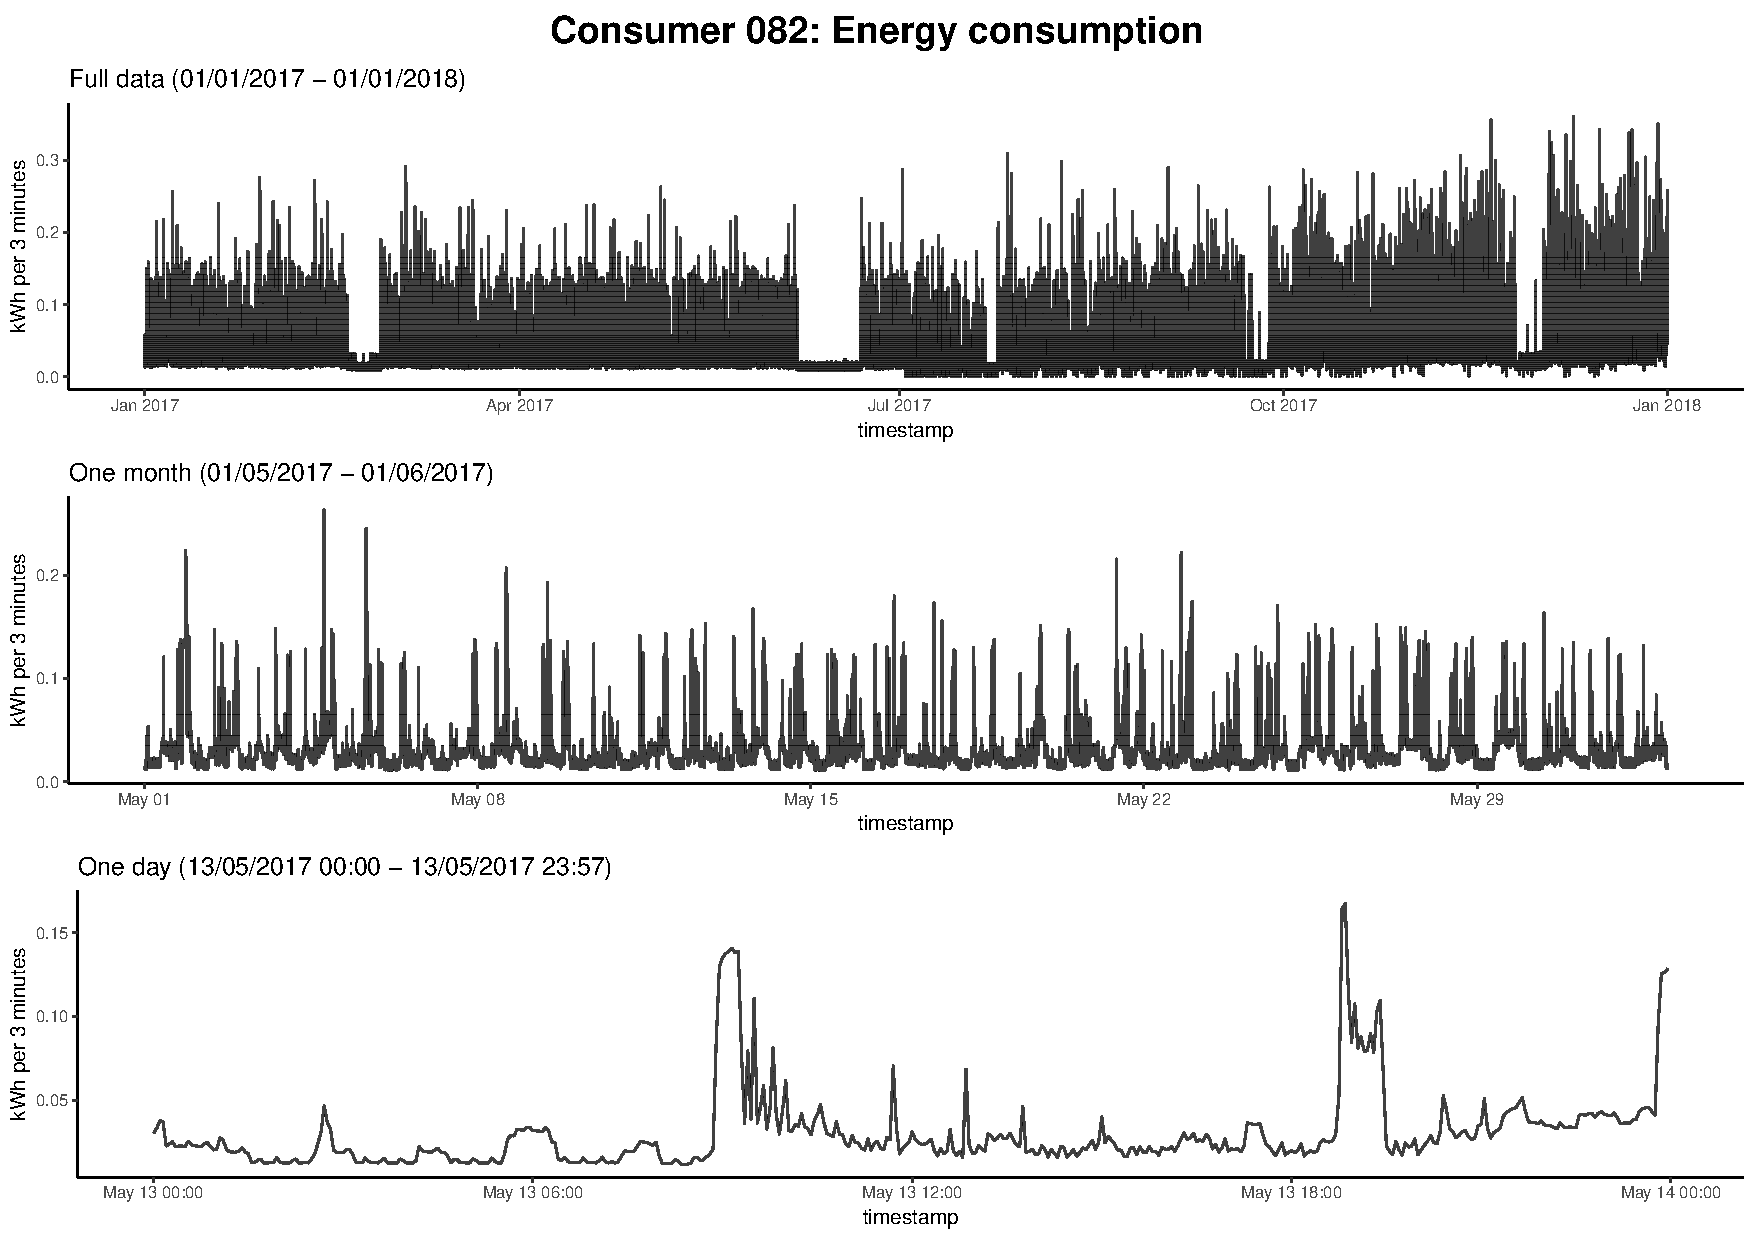
\includegraphics[width=\textwidth]{thesis/graphs/timeseries/c082_cons.pdf}
\caption[Energy consumption recordings of consumer~082]{Energy consumption recordings of consumer~082. The first panel shows the full year 2017, the second panel zooms in to one month (May), and the third panel zooms in to one day (May, 13). \quantnet\href{https://github.com/QuantLet/BLEM/tree/master/BLEMplotEnergyData}{BLEMplotEnergyData}}
\label{Fig:energycons_c082}
\end{figure}

Notably, there are two extended (in March and June) and three shorter periods (in July, September, and December) of clearly distinguishable low consumption and low fluctuation levels. The most likely explanations for these low, stable energy consumption periods are holidays, in which the household members are on vacation and leave appliances that are on standby or always turned on as the only energy consumers. This exemplifies the fact, that household members' behaviour is the biggest driver of fluctuations in the energy consumption of a household and the almost only cause for uncertainty in the time series.

Interestingly, the consumption time series of consumer~082 shows an increase in mean consumption starting with October 2017. This could be explained by colder outside temperatures. However, within the first quarter of 2017, no equivalent decrease in the mean energy consumption can be seen. Therefore, the reason for this increase might be newly acquired household appliances which are increasingly used with the approaching winter as the household members spend more time indoors.

The second panel zooms to just one month making daily fluctuation patterns already visible. In May there seem to be no abnormal consumption patterns. There are a few peaks in the first and third week of May that stand out, but no longer periods of very low energy consumption are present. More interestingly seems to be the last panel, which zooms in to just one day of energy consumption, i.e., May 13, 2017. This day was chosen for no particular reason other than that it is more or less in the middle of the month shown in the second panel. May 13, however, nicely exemplifies a usual pattern of energy consumption: There is low and rather stable energy consumption from midnight until about 7.30 a.m.~which only fluctuates in a systematic and repeated way. Most probably, this ``base consumption" is caused by appliances in standby and ``always on" appliances, such as a fridge and/or freezer. At around 7.30 a.m., the household members probably wake up and the energy consumption spikes for the next 30 minutes -- the light is turned on, coffee is made, the stove is turned on, and maybe a flow heater is used to shower with hot water. As the household members leave the house (May 13 is a Monday), the consumption slowly decreases again. In the evening at about 6.30 p.m.~energy consumption spikes again, probably caused by dinner preparations (and the usage of a microwave or stove). Not intuitively explainable, however, is the spike which is visible just before midnight. This spike, again, highlights the extreme uncertainty contained in individual household energy consumption. It is mostly caused by human behavior, which can seem quite erratic by just looking at energy consumption patterns without context.

To get a better impression of the representativity of consumer~082's energy consumption, it is compared to the other data sets available for this study. Figure~\ref{Fig:cons_total_consumption} shows the total energy consumption in  2017 of all consumers in kWh. As can be seen, consumer~082 (labelled c082 in Figure~\ref{Fig:cons_total_consumption}) is at the lower end of the top quartile of the total energy consumption distribution across all consumers. The household's total energy consumption in 2017 was 6,753 kWh. According to \citet{Stromspiegel:2017}, this number corresponds to a category D five-person household (on a scale from A (very low) to G (very high energy consumption)) that is heating its water with electricity. That means, the household of consumer~082 is either very big or has a comparatively very high energy consumption. Consumer~067, on the contrary, is remarkable as total consumption here is with only 40 kWh quite close to zero. At the high end of total consumption is consumers 025 with almost five times the total consumption of the average consumer in this data sets. Summary statistics for the total energy consumption of consumer households in 2017 can be found in Appendix~\hyperlink{AppB1:Tables:totalcons}{B1}.
%
\begin{figure}[htbp]
 \centering
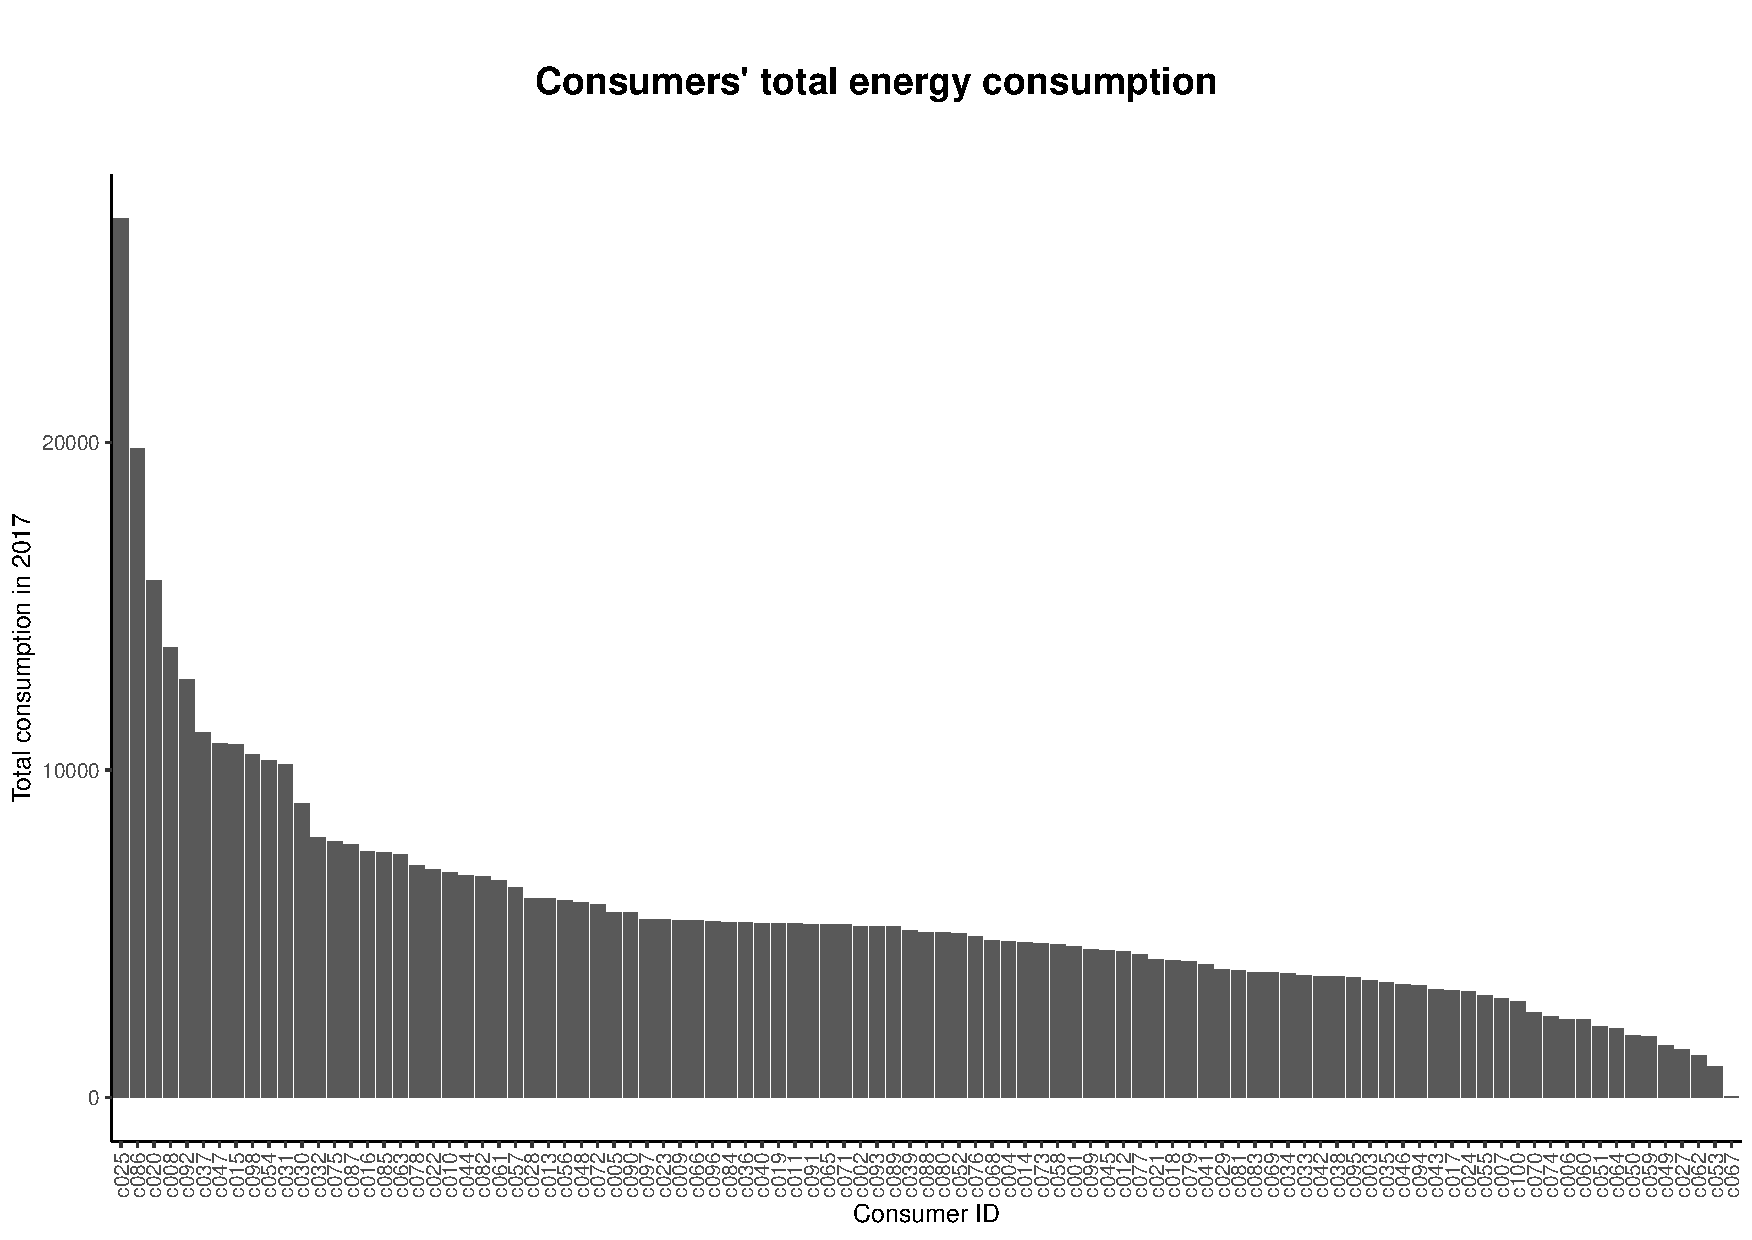
\includegraphics[width=\textwidth]{thesis/graphs/consumer_totalconsumption.pdf}
\caption[Consumers' total energy consumption in 2017]{Consumers' total energy consumption (in kWh) in 2017 ordered from high to low. \quantnet\href{https://github.com/QuantLet/BLEM/tree/master/BLEMdescStatEnergyData}{BLEMdescStatEnergyData}}
\label{Fig:cons_total_consumption}
\end{figure}
%

Figure~\ref{Fig:cons_boxplots_consumption} offers another perspective on the consumers' energy consumption. The figure shows a boxplot for each consumer's distribution of energy consumption per 3-minute interval. That means, the median line in the boxplot of a consumer is the consumer's median consumption per 3-minute interval, while the box encloses the interquartile range (IQR) of the 3-minute consumption values of this particular consumer. It is apparent, that the IQR is for almost all consumers relatively small compared to the total range of their consumption values. All points plotted above the boxplots' whiskers are consumption values greater than the third quartile plus 1.5 $\times$ IQR. This again shows that there is a substantial amount of extreme values -- for which the description ``outlier" not necessarily fits as they obviously occur quite often -- which are, most likely, hard to predict with standard forecasting methods.
%
\begin{figure}[htbp]
 \centering
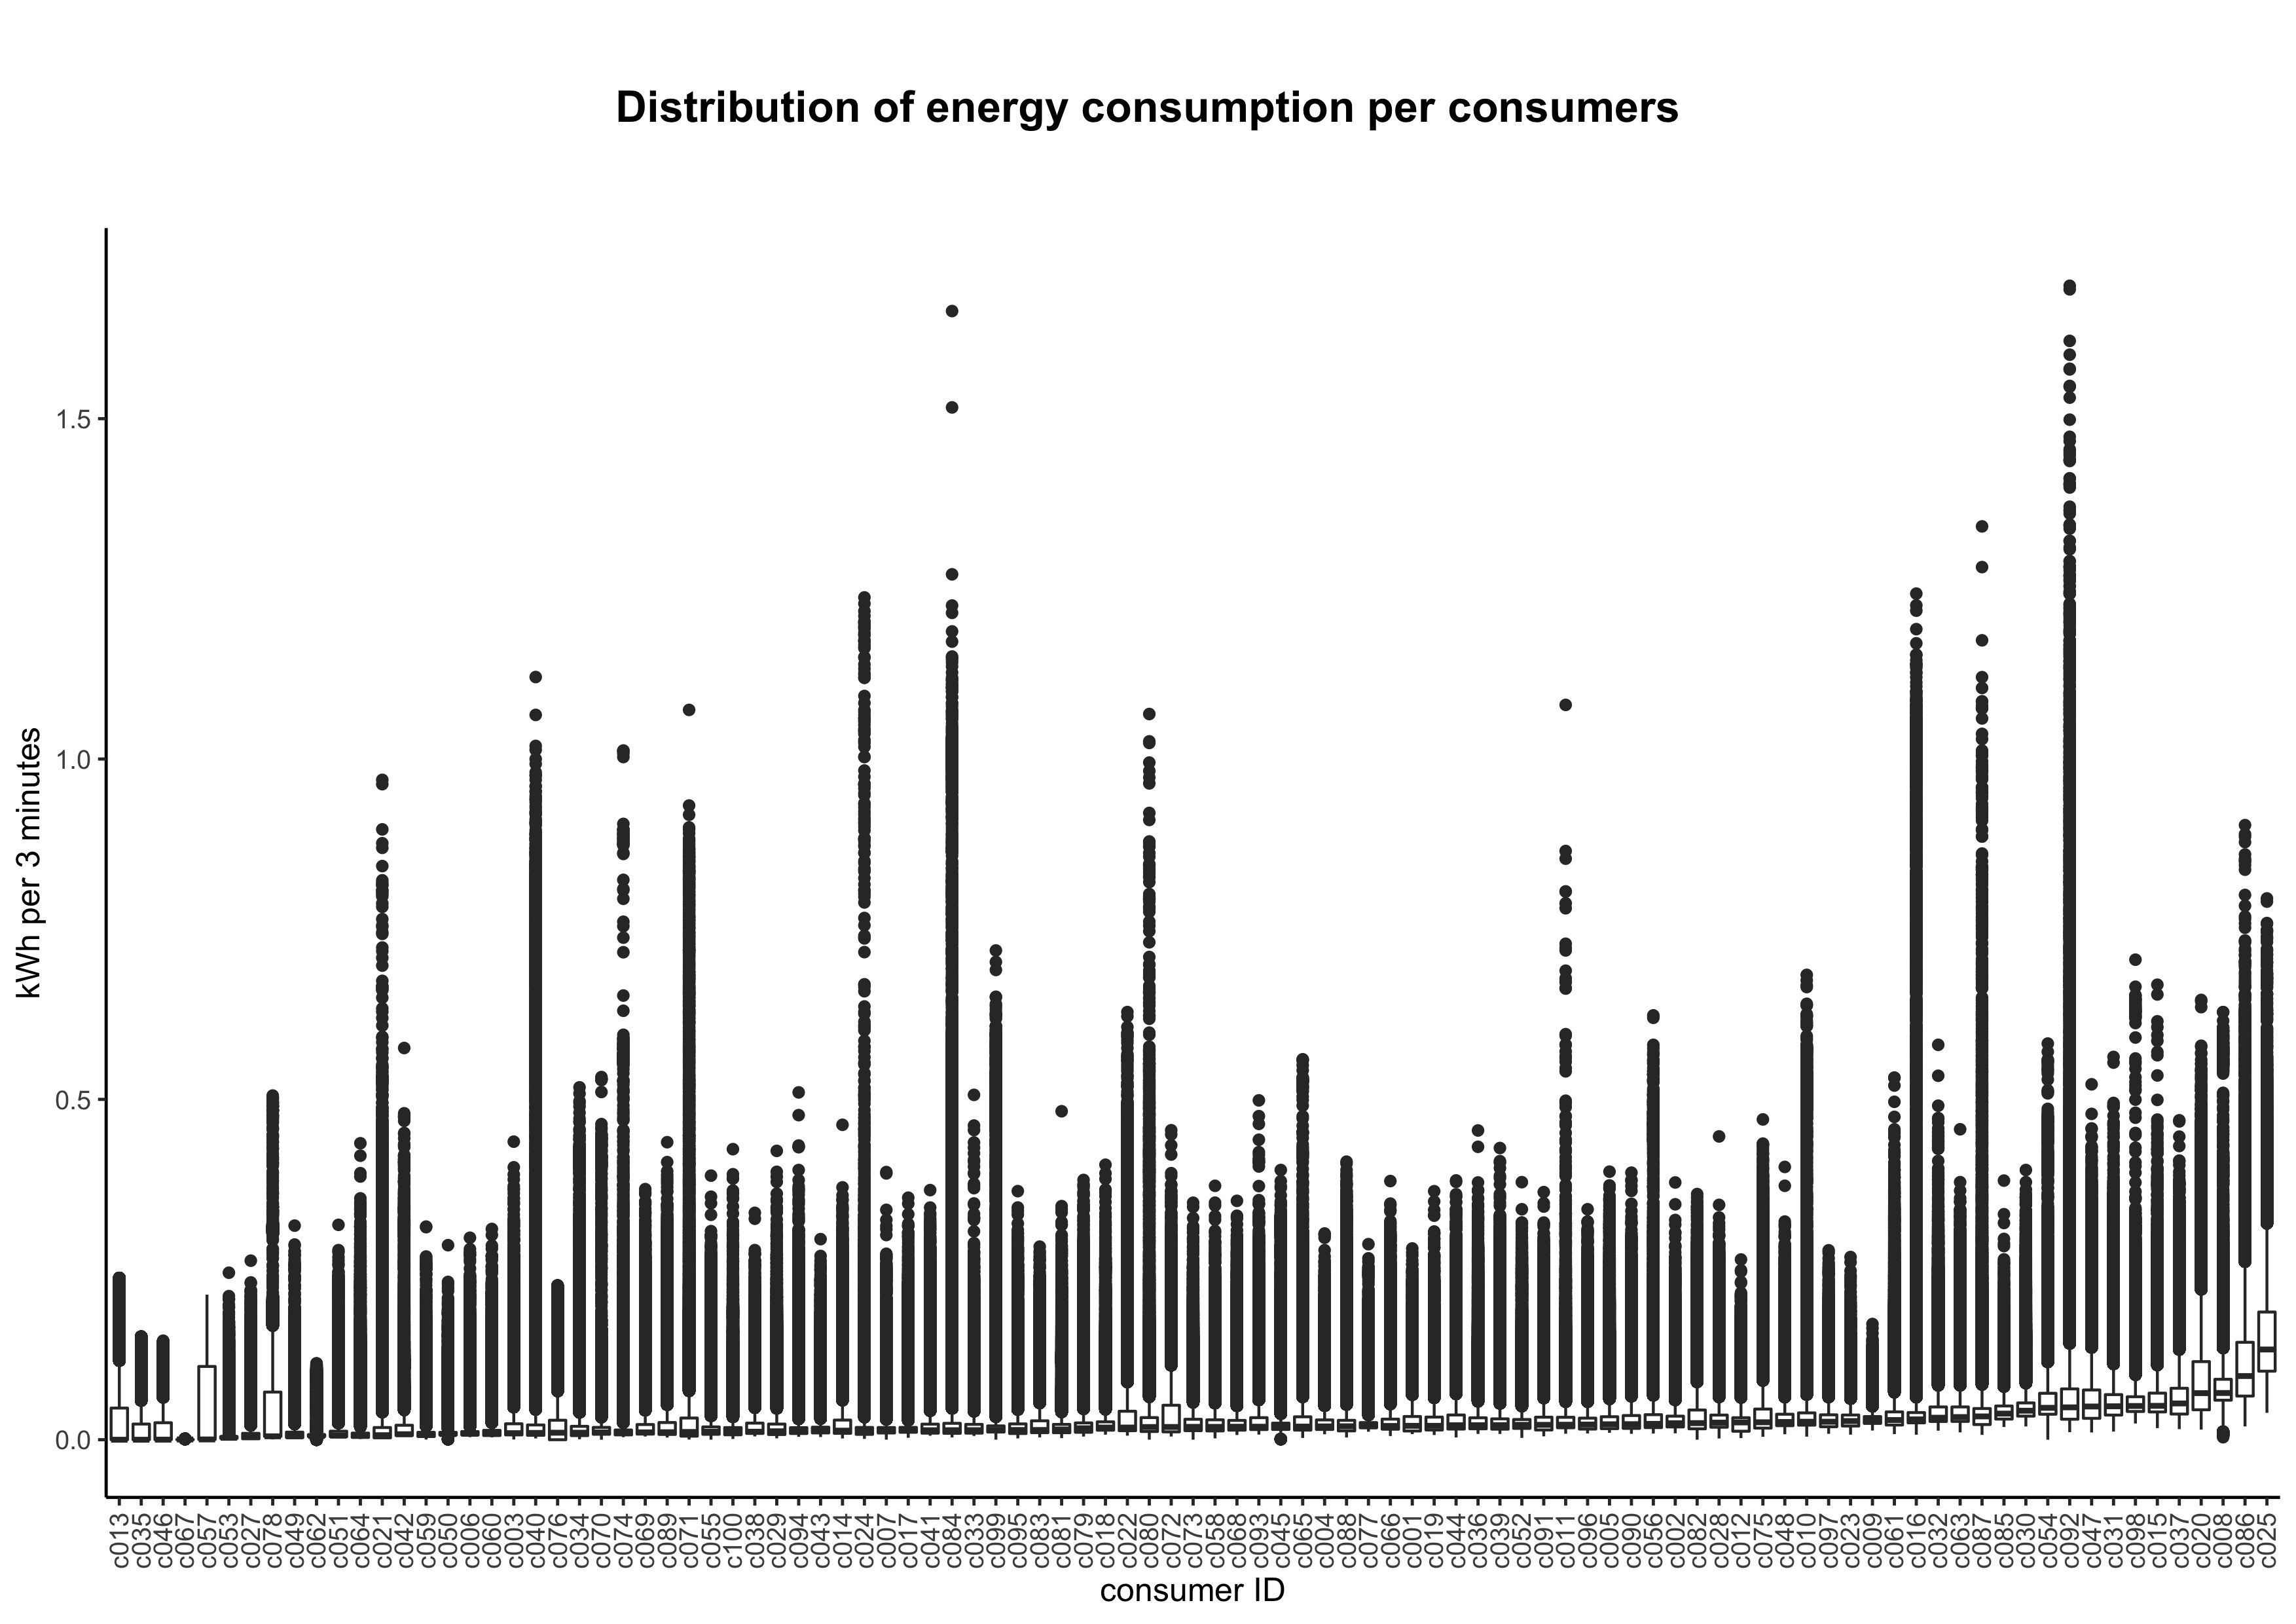
\includegraphics[width=\textwidth]{thesis/graphs/consumer_boxplots_consumption.jpg}
\caption[Boxplots of each consumer's energy consumption in kWh/3-minute interval]{Boxplots of each consumer's energy consumption in kWh per 3-minute interval. \quantnet\href{https://github.com/QuantLet/BLEM/tree/master/BLEMdescStatEnergyData}{BLEMdescStatEnergyData}}
\label{Fig:cons_boxplots_consumption}
\end{figure}



%%%%%%%%%%%
\newpage
\subsubsection{Prosumer data sets}

Interestingly, the prosumer data sets show very different consumption patterns than pure consumers. This may be due to the fact, that the recorded energy consumption per 3-minute interval is the net value of the actual energy consumption minus the energy production in the same interval. For example, if prosumer~024's recorded consumption value is 0.021 kWh in the time period from 2017-05-13 06:03:00 to 06:06:00, and its energy production in the same interval is 0.018 kWh (which is not recorded and therefore not known), its actual energy consumption in that time interval is 0.039 kWh. However, this actual energy consumption is unknown as the energy production per 3-minute interval is not recorded. Only a surplus of energy production over consumption would be recorded as an increase in the energy out readings (see Table~\ref{Tab:p089}) -- which is not the case in this example.

Visual inspection of the consumption time series of the prosumer data sets already reveals that the consumption patterns in most cases do not resemble the consumer households' consumption patterns. Generalized, four types of consumption patterns can be found in the prosumer data: (1) The net energy consumption of the prosumer is zero at night, starts to increase at around 6 a.m., fluctuates over daytime, and decreases to zero again at around 6 p.m. (see exemplary prosumer 004 in Figure~\ref{Fig:prosenergycons_peculiar}). (2) The net energy consumption is mostly non-zero and fluctuates (in a regular pattern) at low levels with occasional net consumption spikes (see exemplary consumer 050 in Figure~\ref{Fig:prosenergycons_peculiar}). This is the most generic type of prosumer energy consumption patterns. (3) The net consumption is for most of the year zero (see exemplary prosumer 061 in Figure~\ref{Fig:prosenergycons_peculiar}). This may be due to a surplus in net energy production. (4) The net energy consumption is mostly non-zero, fluctuates very little at a relatively high level (see exemplary prosumer 093 in Figure~\ref{Fig:prosenergycons_peculiar}), and the net energy consumption drops only occasional from this high level. Type (1) and (2) represent the majority of data sets. Type (1) is very easily identifiable and represents 30~\% of the data sets. Type (2) is more generic and therefore comprises more heterogenic patterns with 56~\% of the data sets belonging to this type. Type (3) and (4), exemplary shown in the lower two panels of Figure~\ref{Fig:prosenergycons_peculiar}, only represent a minority of the data sets.

\begin{sidewaysfigure}[htbp]
    \centering
    \begin{minipage}[h]{\dimexpr.5\textheight-0.15em}
    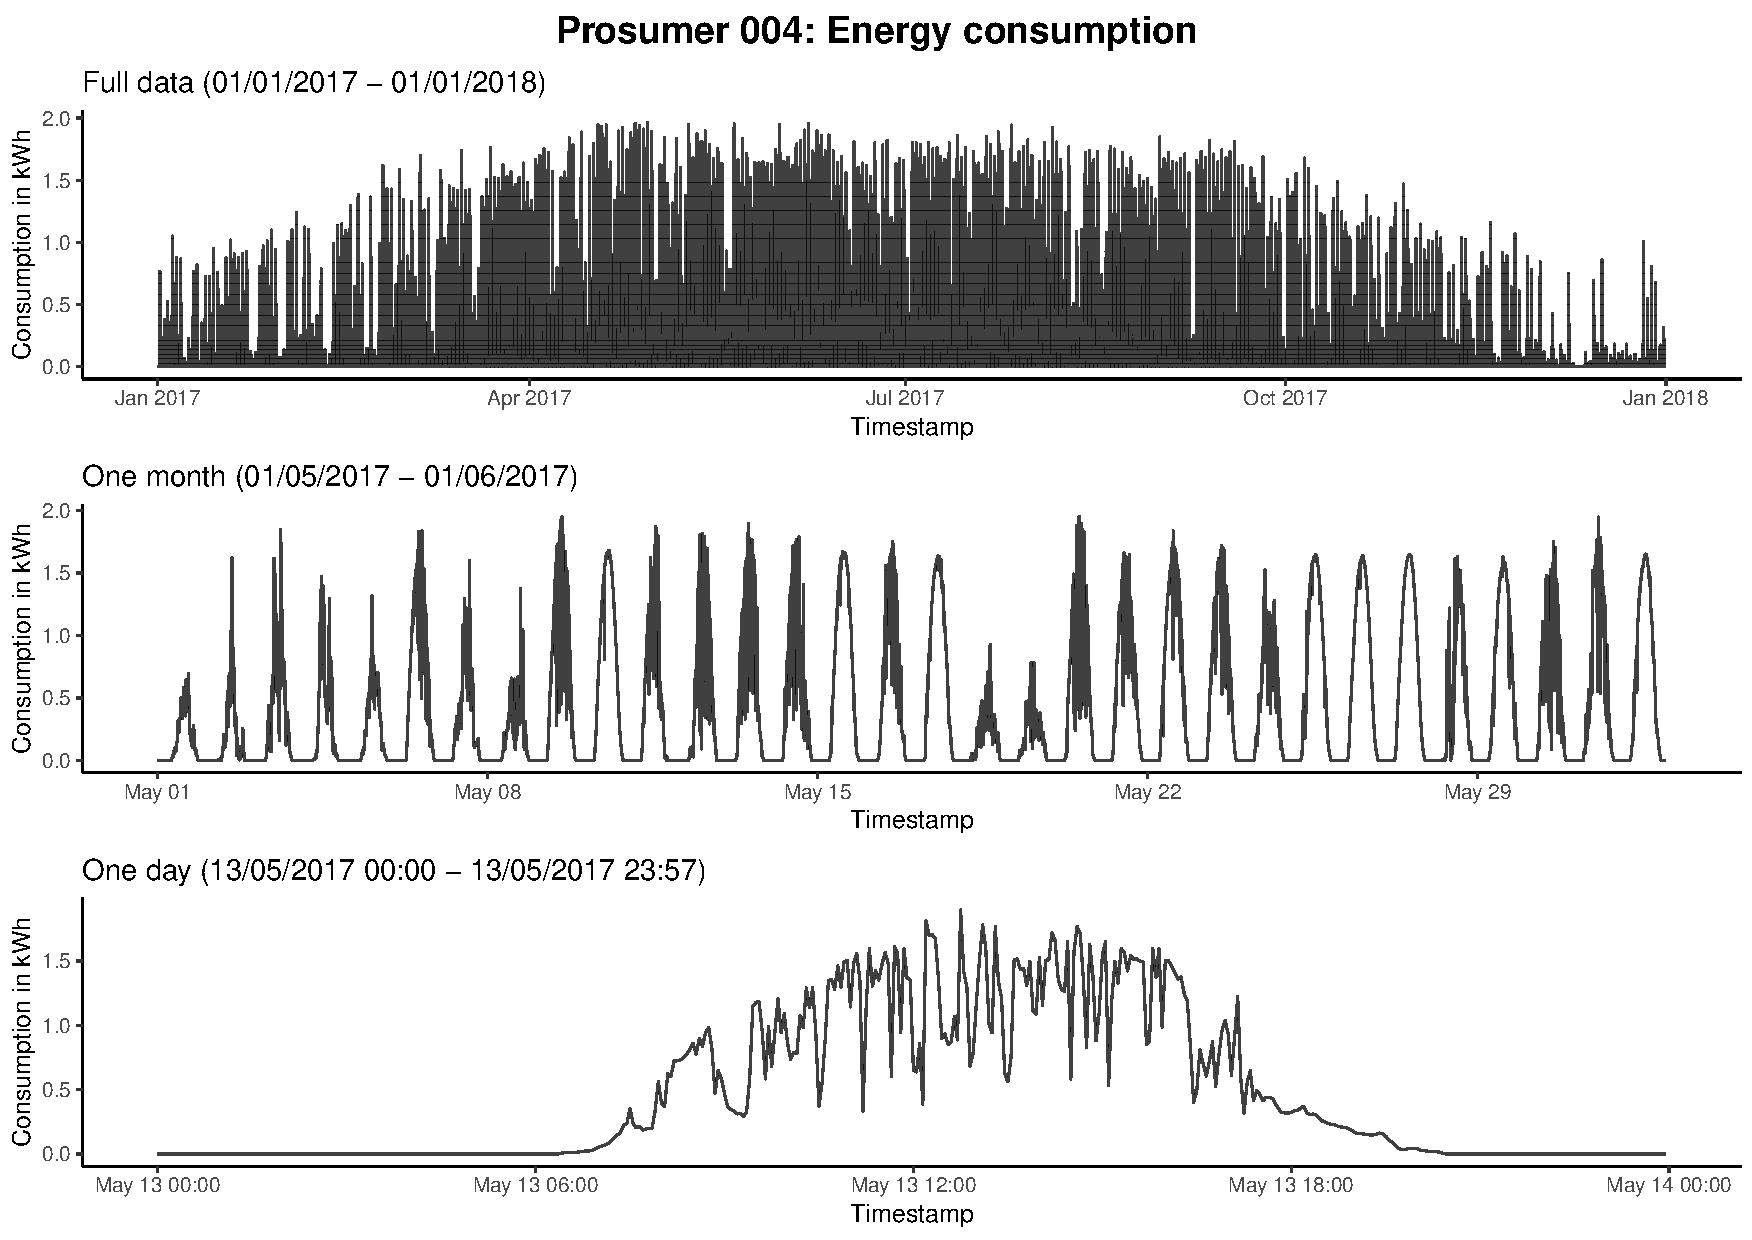
\includegraphics[width=\textwidth]{thesis/graphs/timeseries/p004_cons.pdf}
    \end{minipage}
    \begin{minipage}[h]{\dimexpr.5\textheight-0.15em}
    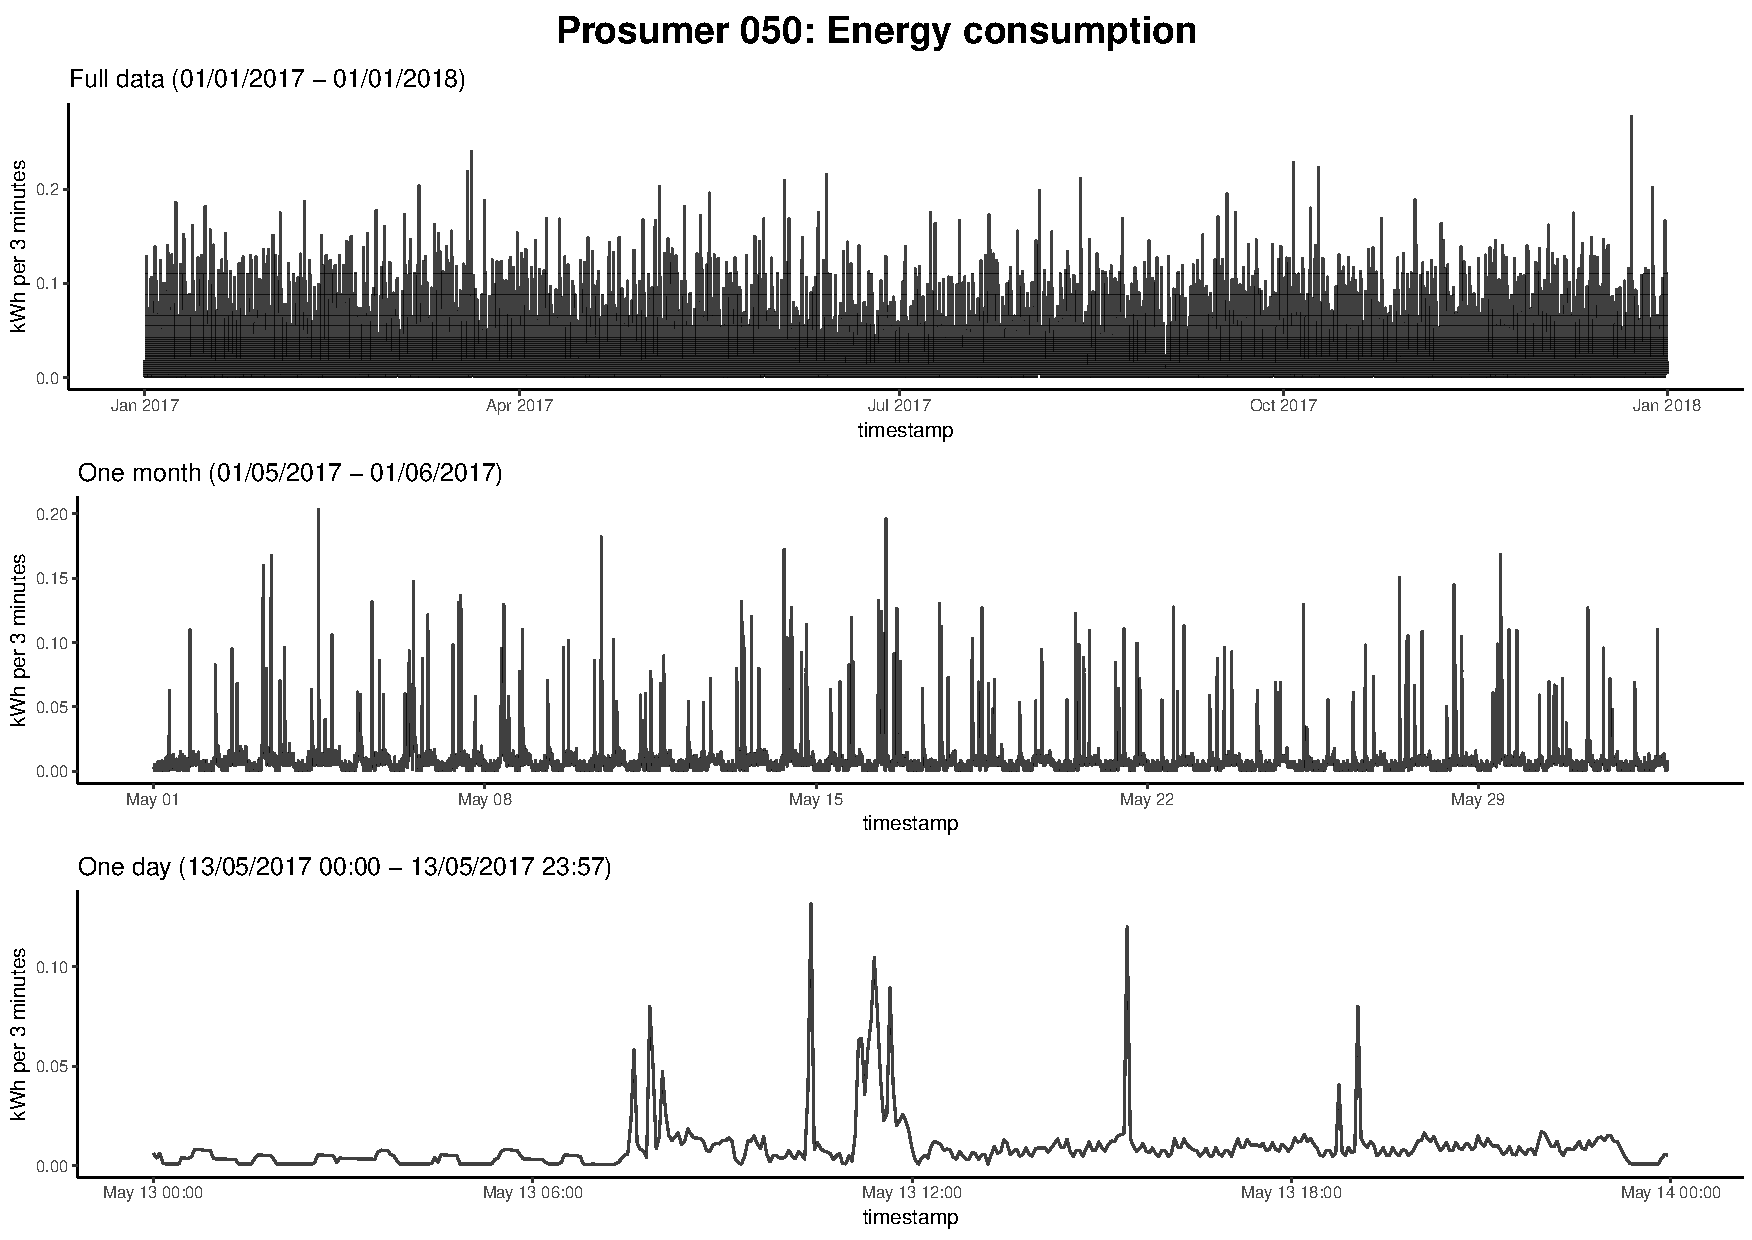
\includegraphics[width=\textwidth]{thesis/graphs/timeseries/p050_cons.pdf}
    \end{minipage}\\
    
    \begin{minipage}[h]{\dimexpr.5\textheight-0.15em}
    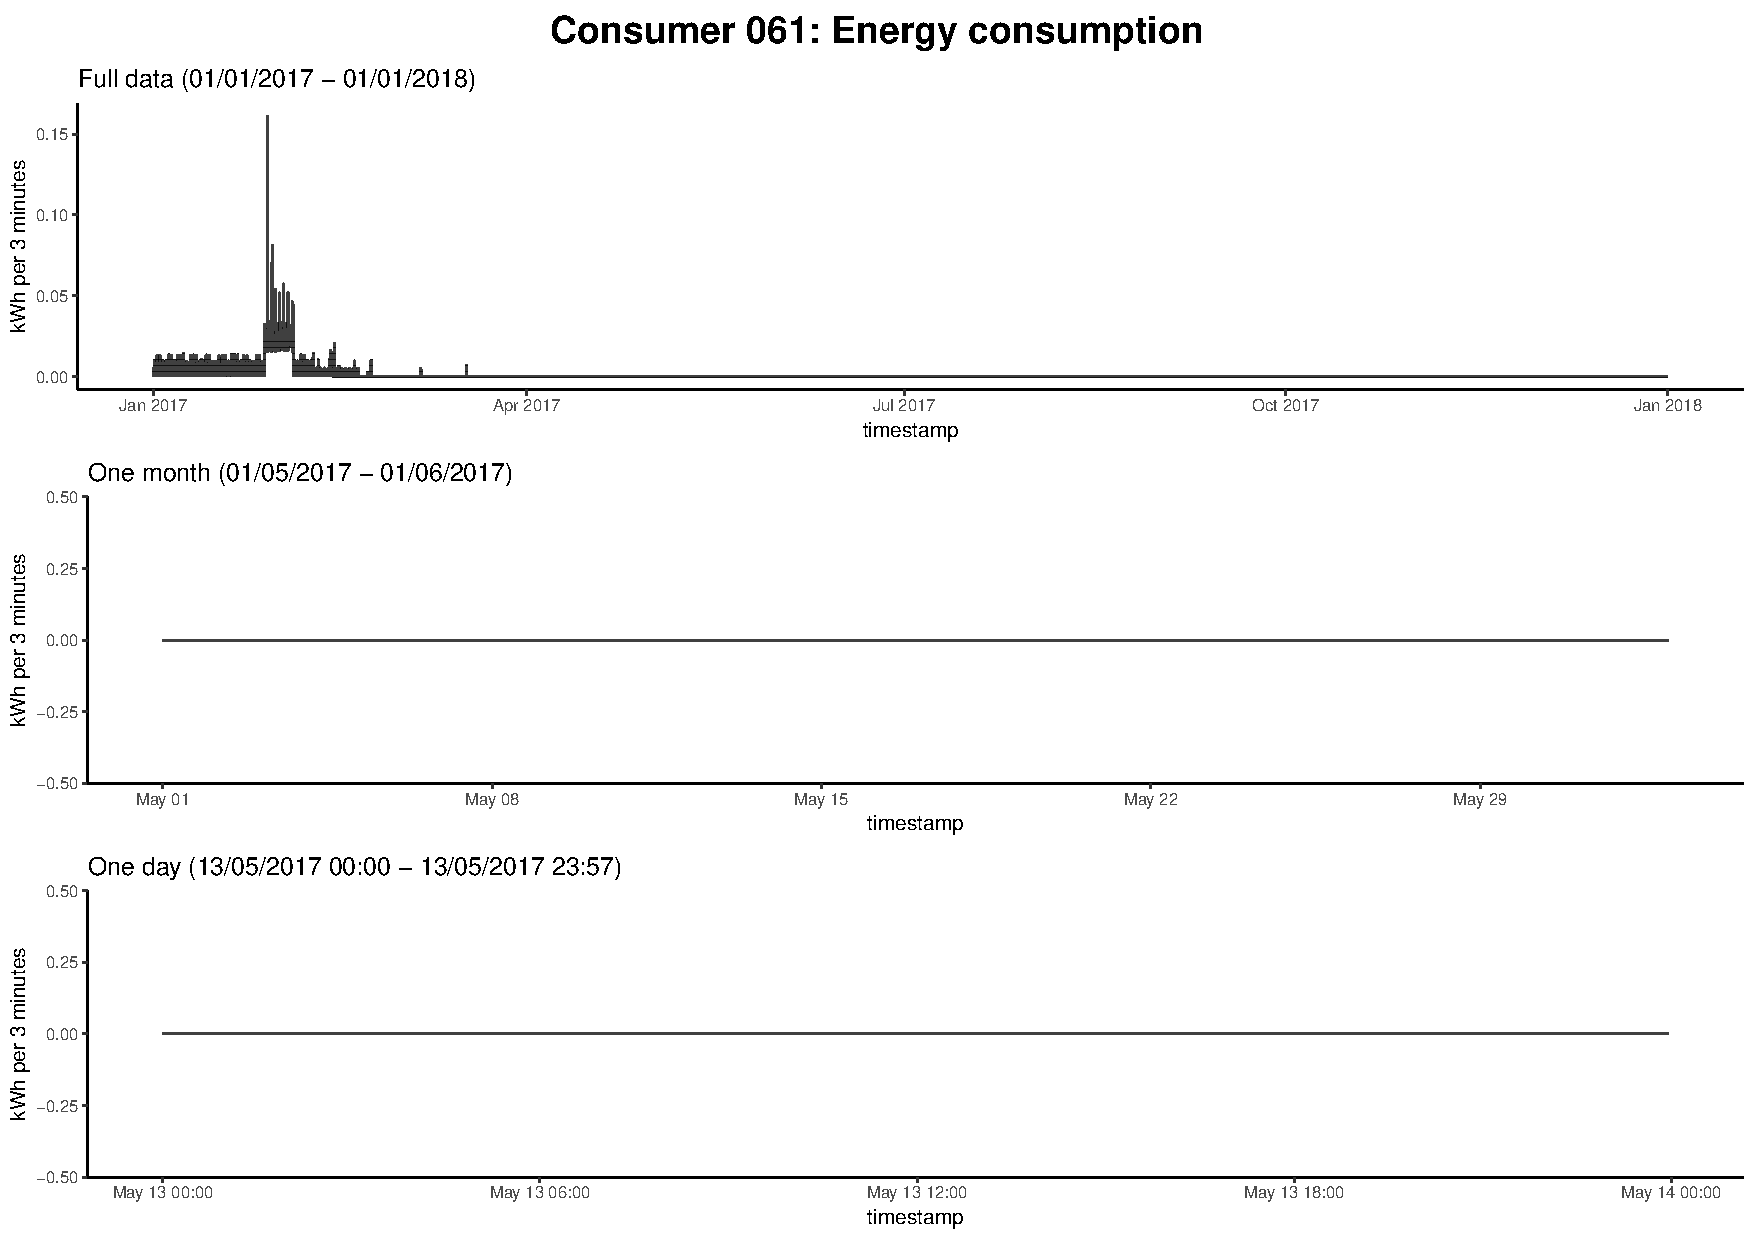
\includegraphics[width=\textwidth]{thesis/graphs/timeseries/p061_cons.pdf}
    \end{minipage}
    \begin{minipage}[h]{\dimexpr.5\textheight-0.15em}
    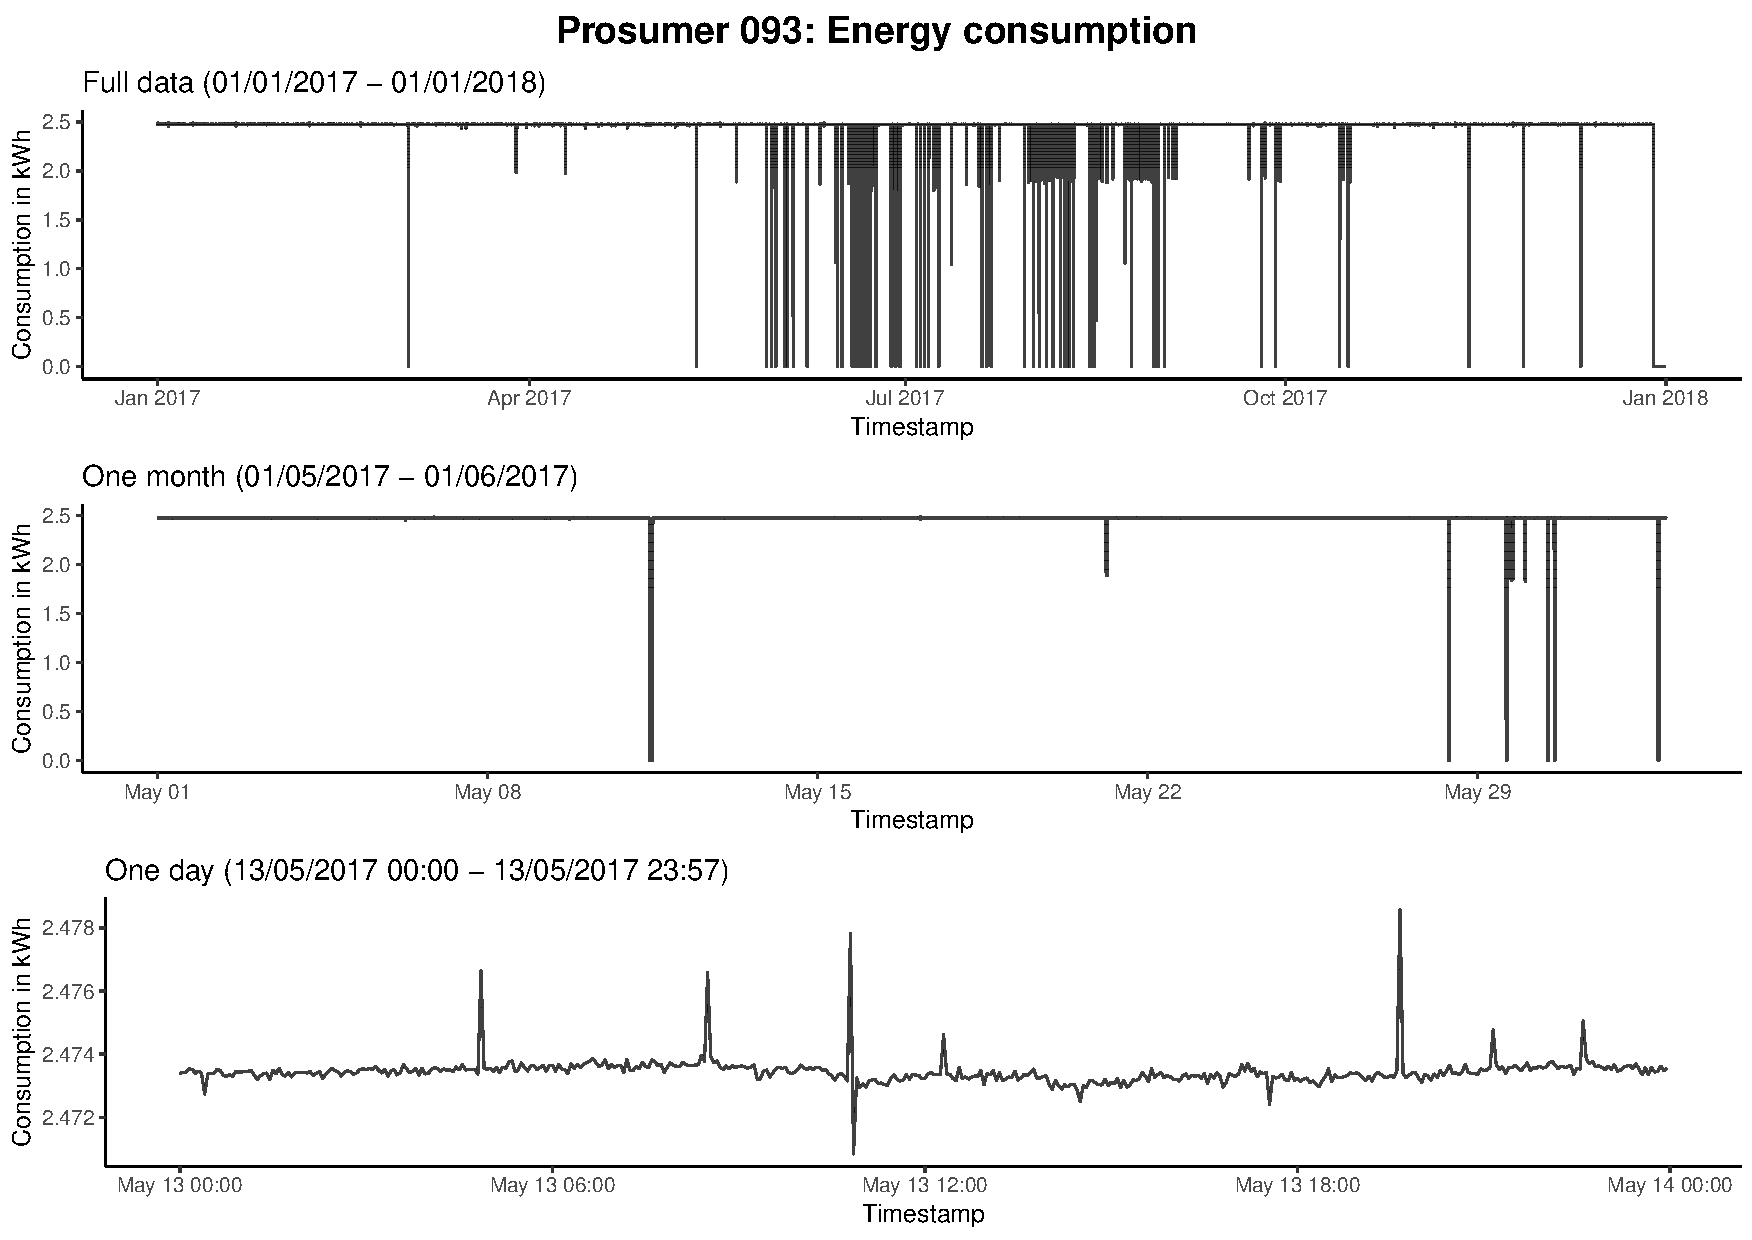
\includegraphics[width=\textwidth]{thesis/graphs/timeseries/p093_cons.pdf}
    \end{minipage}
    
    \caption[Examples for types of prosumer energy consumption patterns]{Exemplary prosumers representing different types of prosumer energy consumption patterns. \quantnet\href{https://github.com/QuantLet/BLEM/tree/master/BLEMplotEnergyData}{BLEMplotEnergyData}}
    \label{Fig:prosenergycons_peculiar}
\end{sidewaysfigure}

In conclusion, it becomes clear that the net energy consumption of prosumers may exhibit very different patterns than the energy consumption of consumers. This exacerbates the prediction task for prosumers significantly. Furthermore, the total consumption of prosumers follows a very different distribution than the total consumption of consumers. The maximum total net consumption of a prosumer was 424,893 kWh, which is 15 times more than the maximum total consumption of a consumer. 19 out of 100 prosumers net consumed more energy than the biggest consumer household contained in the data. Also, the dispersion of the total net consumption is much higher with an IQR of 22,149 kWh for prosumers' total net consumption compared to an IQR of 2,542 kWh for consumers' total consumption in 2017.

\begin{figure}[htbp]
 \centering
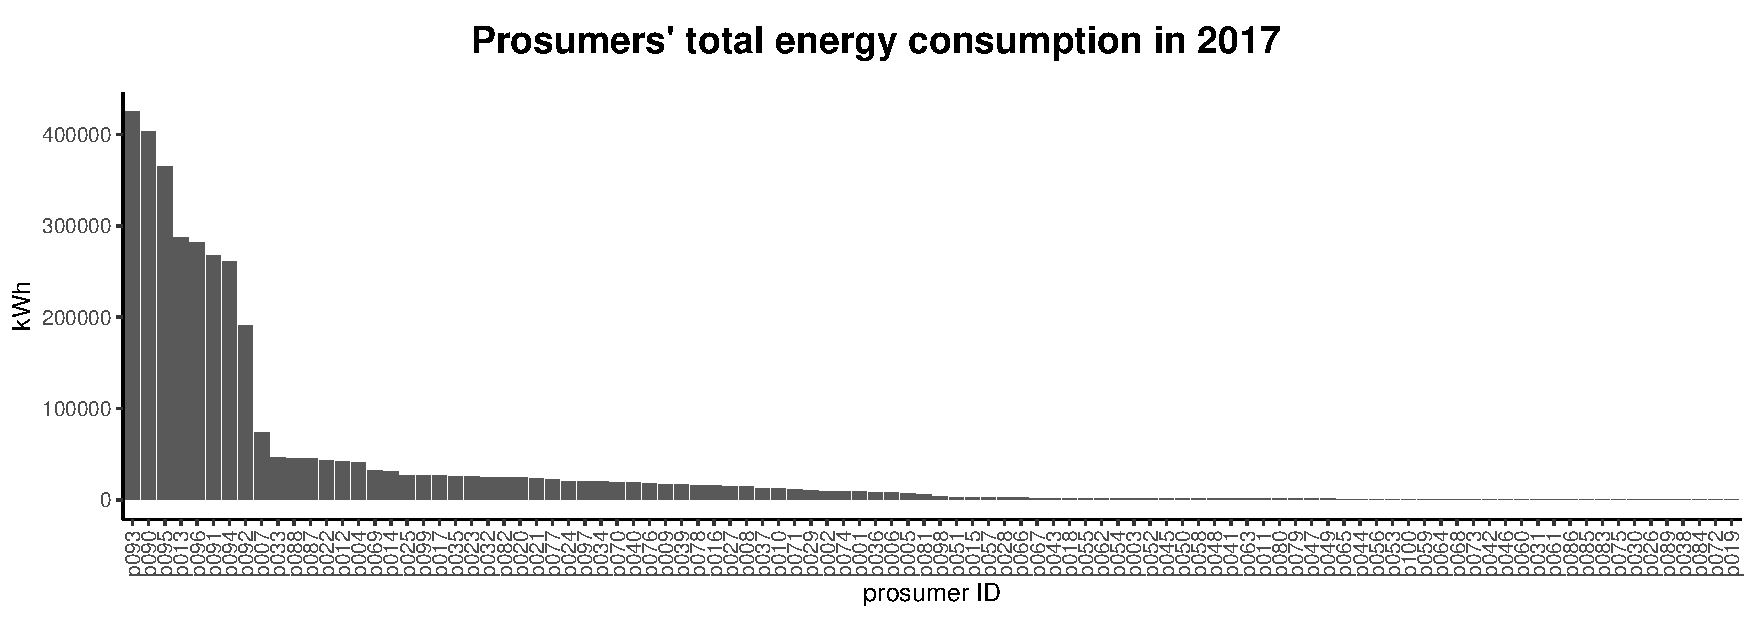
\includegraphics[width=\textwidth]{thesis/graphs/prosumer_totalconsumption.pdf}
\caption[Prosumers’ total energy consumption in 2017]{Prosumers’ total energy consumption (in kWh) in 2017 ordered from high to low. \quantnet\href{https://github.com/QuantLet/BLEM/tree/master/BLEMdescStatEnergyData}{BLEMdescStatEnergyData}}
\label{Fig:pros_total_consumption}
\end{figure}

Finally, Figure~\ref{Fig:pros_boxplots_consumption} offers another perspective on the heterogeneity of the prosumer data sets. The figure shows a boxplot for each prosumer's energy consumption values per 3-minute interval. The prosumers are sorted on the x-Axis by their median net energy consumption. As can be seen, while the median for the majority of the prosumers is relatively close to zero, the IQR and the total range of net consumption values differs substantially between prosumers. Approximately the same range of net consumption values per 3-minute interval can be accompanied by a median of 0.0003 kWh (see p088 in Figure~\ref{Fig:pros_boxplots_consumption}) or by a median of 1.9110 kWh (see p094 in Figure~\ref{Fig:pros_boxplots_consumption}).

\begin{figure}[htbp]
 \centering
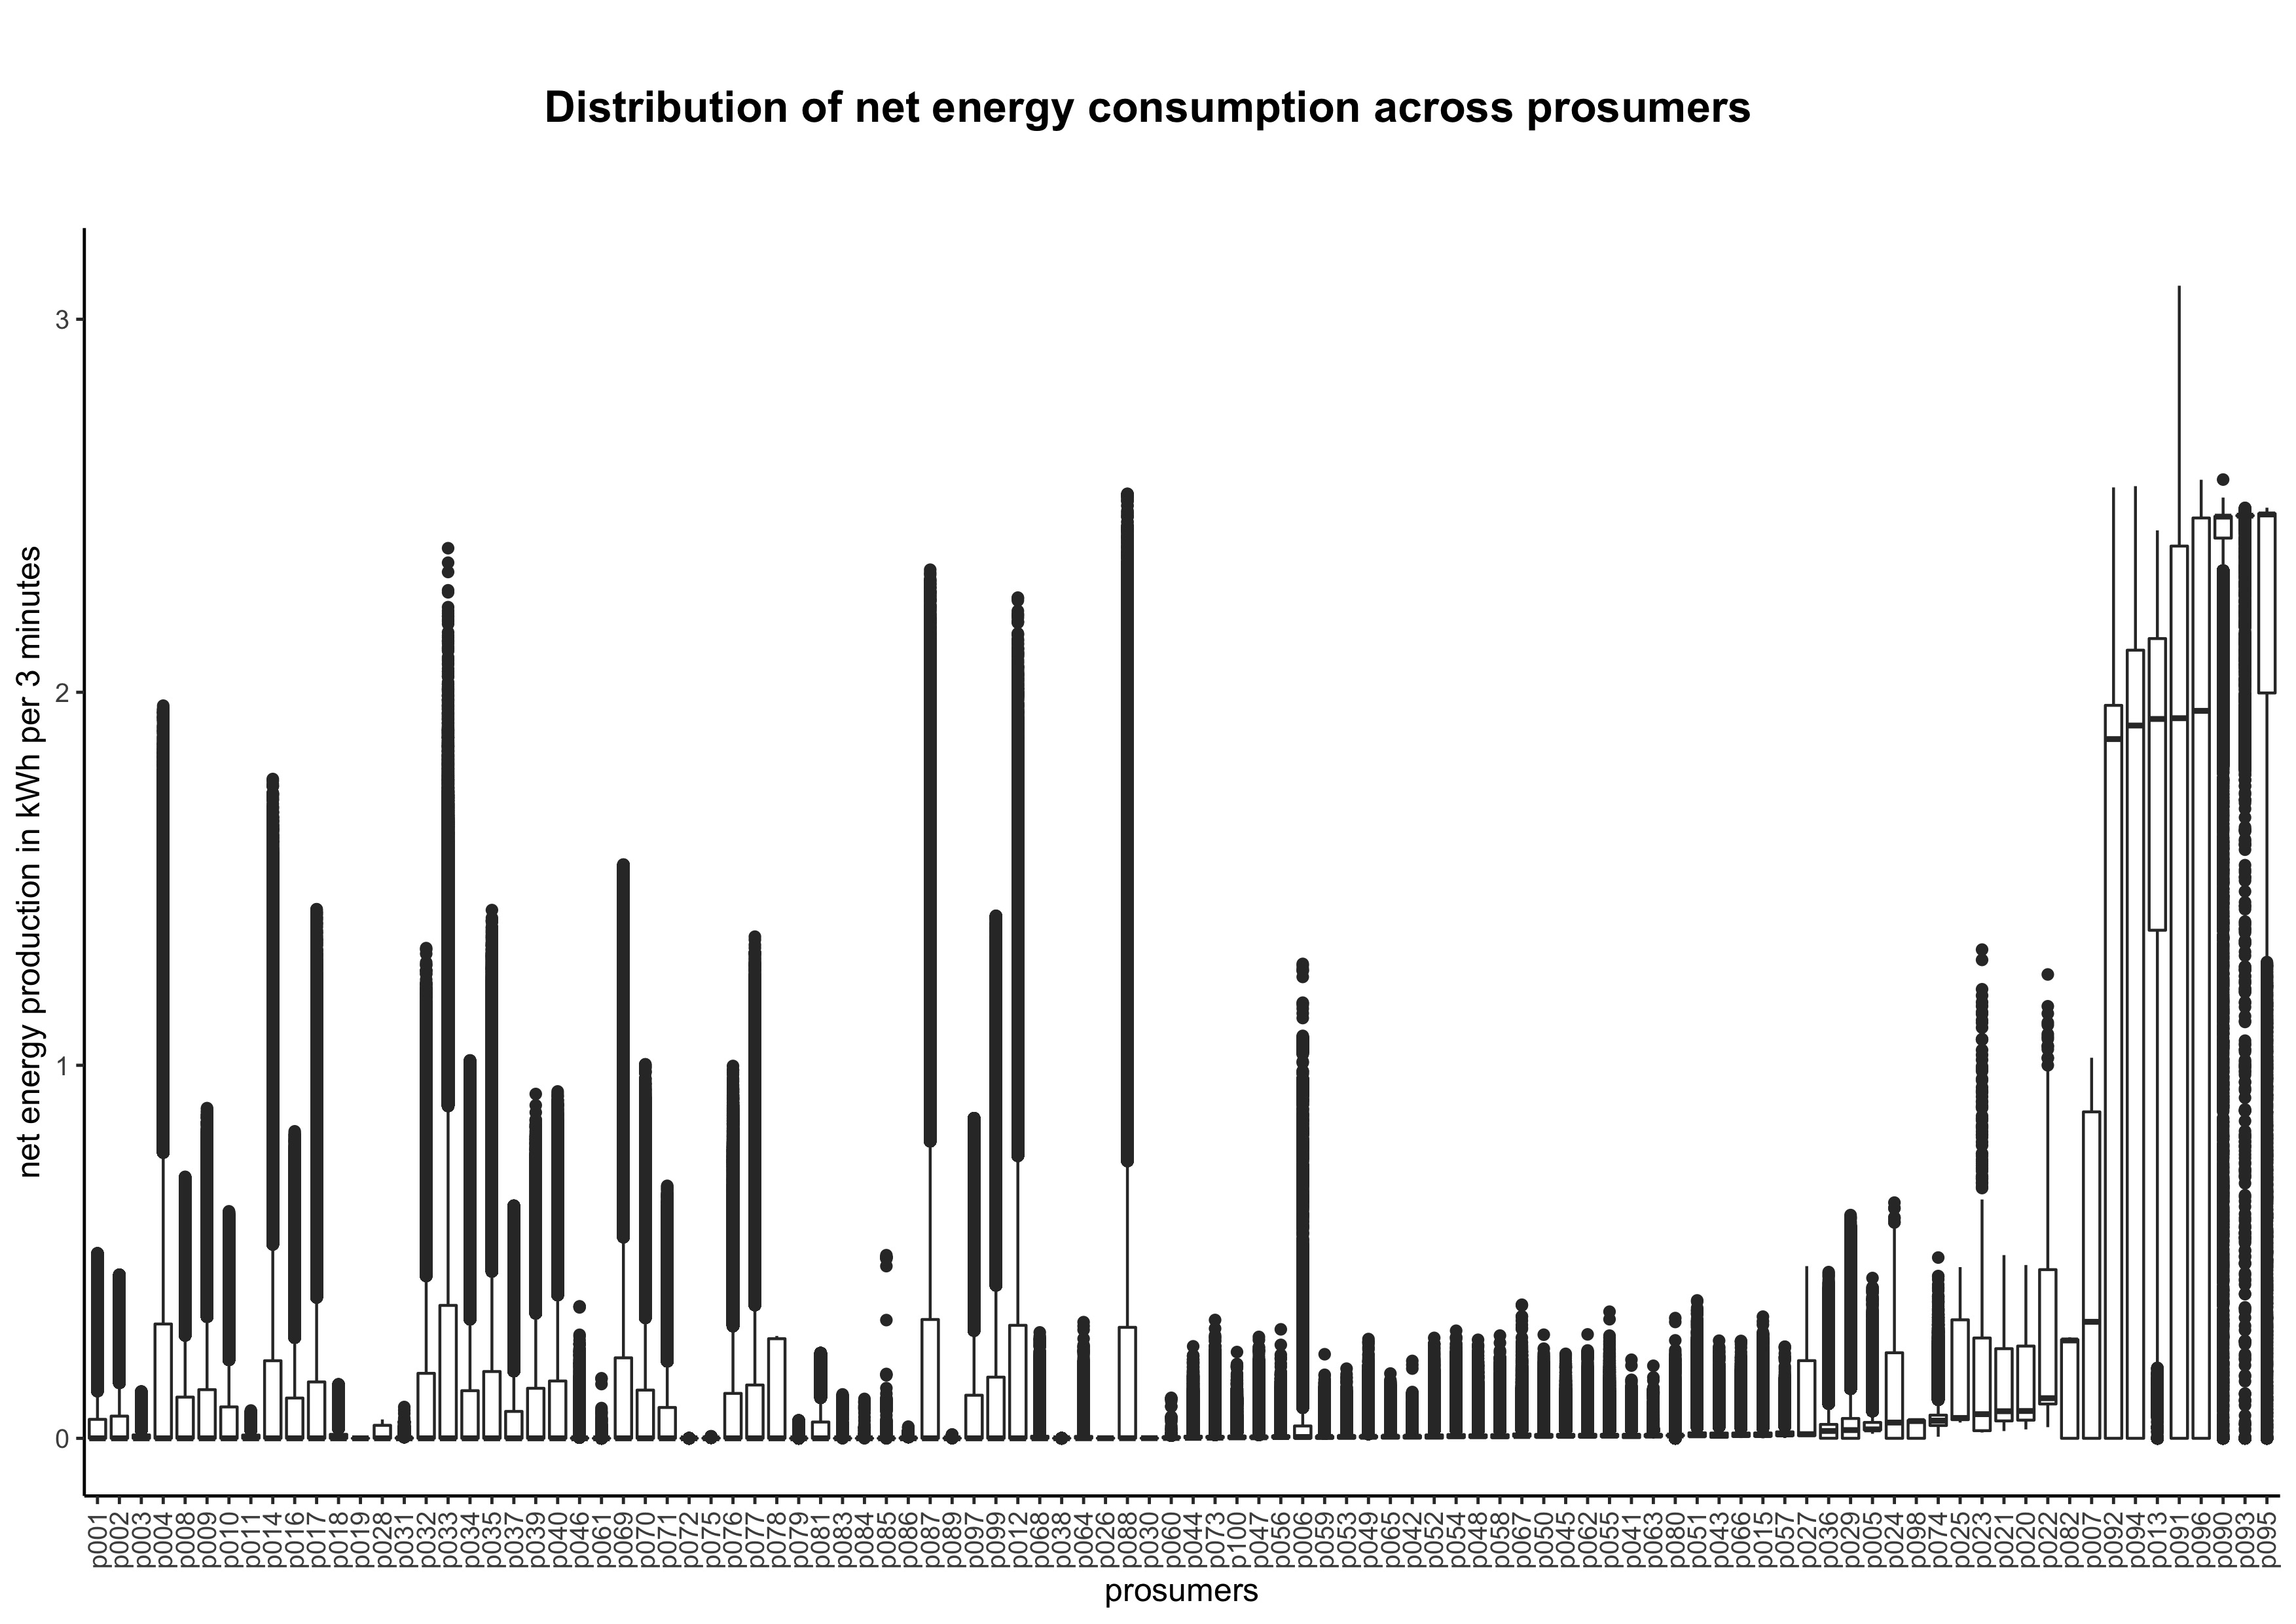
\includegraphics[width=\textwidth]{thesis/graphs/prosumer_boxplots_consumption.jpg}
\caption[Boxplots of each prosumer's net energy consumption in kWh/3-minute interval]{Boxplots of each prosumer's net energy consumption in kWh per 3-minute interval. \quantnet\href{https://github.com/QuantLet/BLEM/tree/master/BLEMdescStatEnergyData}{BLEMdescStatEnergyData}}
\label{Fig:pros_boxplots_consumption}
\end{figure}

Prosumers are defined by the fact, that they not only consume energy but also produce energy -- primarily for their own consumption. However, any surplus in energy production over energy consumption is fed into the grid and, thus, recorded by the smart meter as an increase in the energy out readings. As explained above, these energy out readings are used to compute the net energy production per 3-minute interval by first-differencing. Surprisingly, only 14 out of 100 available prosumer data sets contained non-zero net energy production values at all. This becomes clear when looking at Figure~\ref{Fig:pros_total_production}, which shows the total net energy production of all prosumers. 86 of those prosumers fed zero kWh into the grid during 2017. The top three net energy producing prosumers, however, fed a total of 1,259,686 kWh into the grid, which is more than twice the amount all 100 consumer households consumed together\footnote{Cumulatively, the 100 consumer households, for which data is available, consumed 559,369 kWh in 2017.}. For comparison, a typical photovoltaic (PV) installation on a private residential building with a roof surface area of 150 m$^2$ produces approximately 20,000 kWh per year \citep{energieatlas:2018}.

\begin{figure}[htbp]
 \centering
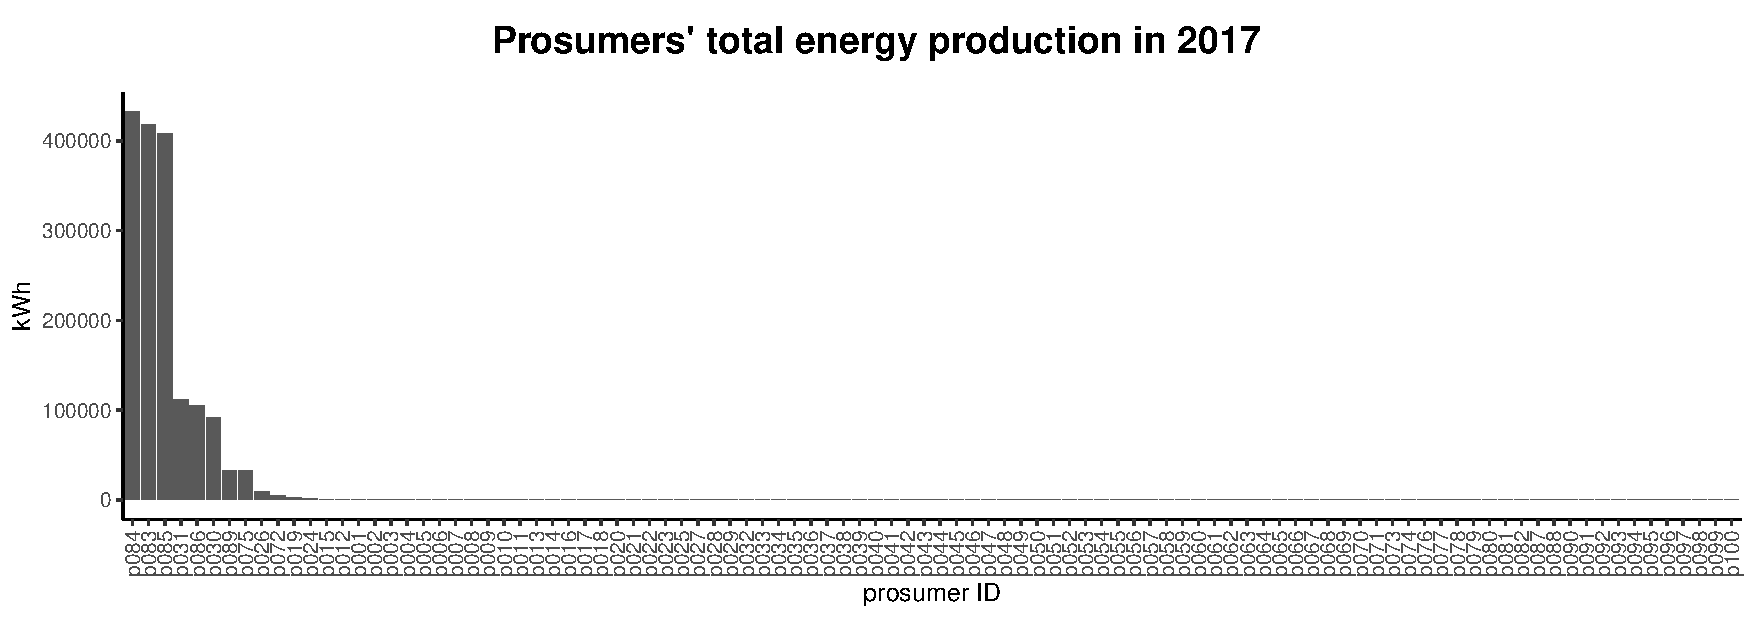
\includegraphics[width=\textwidth]{thesis/graphs/prosumer_totalproduction.pdf}
\caption[Prosumers’ total energy production in 2017]{Prosumers’ total energy production (in kWh) in 2017 ordered from high to low. \quantnet\href{https://github.com/QuantLet/BLEM/tree/master/BLEMdescStatEnergyData}{BLEMdescStatEnergyData}}
\label{Fig:pros_total_production}
\end{figure}

Prosumer~026, for example, has a relatively low total net energy production. However, its net energy production pattern looks like a typical household with a PV installation (see Figure~\ref{Fig:energyconsprod_p026p086}). The net energy consumption is (almost) always zero, while the net energy production on most days rather smoothly increases and decreases throughout the day with occasional drops, probably caused by changes in the cloud cover. Furthermore, the net energy production increases in the summer months and decreases notably in winter.

Compare this to prosumer~086 that has a stable, very high net energy production over the whole course of 2017. There are only a few drops, which are accompanied by a simultaneous net energy consumption (visible by the small blue spikes in the upper panel of the right graph of Figure~\ref{Fig:energyconsprod_p026p086}, whenever the net production drops). Note also the different scales of the y-axis. The net production of prosumer 084 plays in the range of 1 kWh per 3-minute interval while the net production of prosumer~026 barely surpasses 0.4 kWh per 3-minute interval.
%
\begin{sidewaysfigure}[htbp]
\centering
\begin{minipage}[h]{\dimexpr.5\textwidth-0.15em}
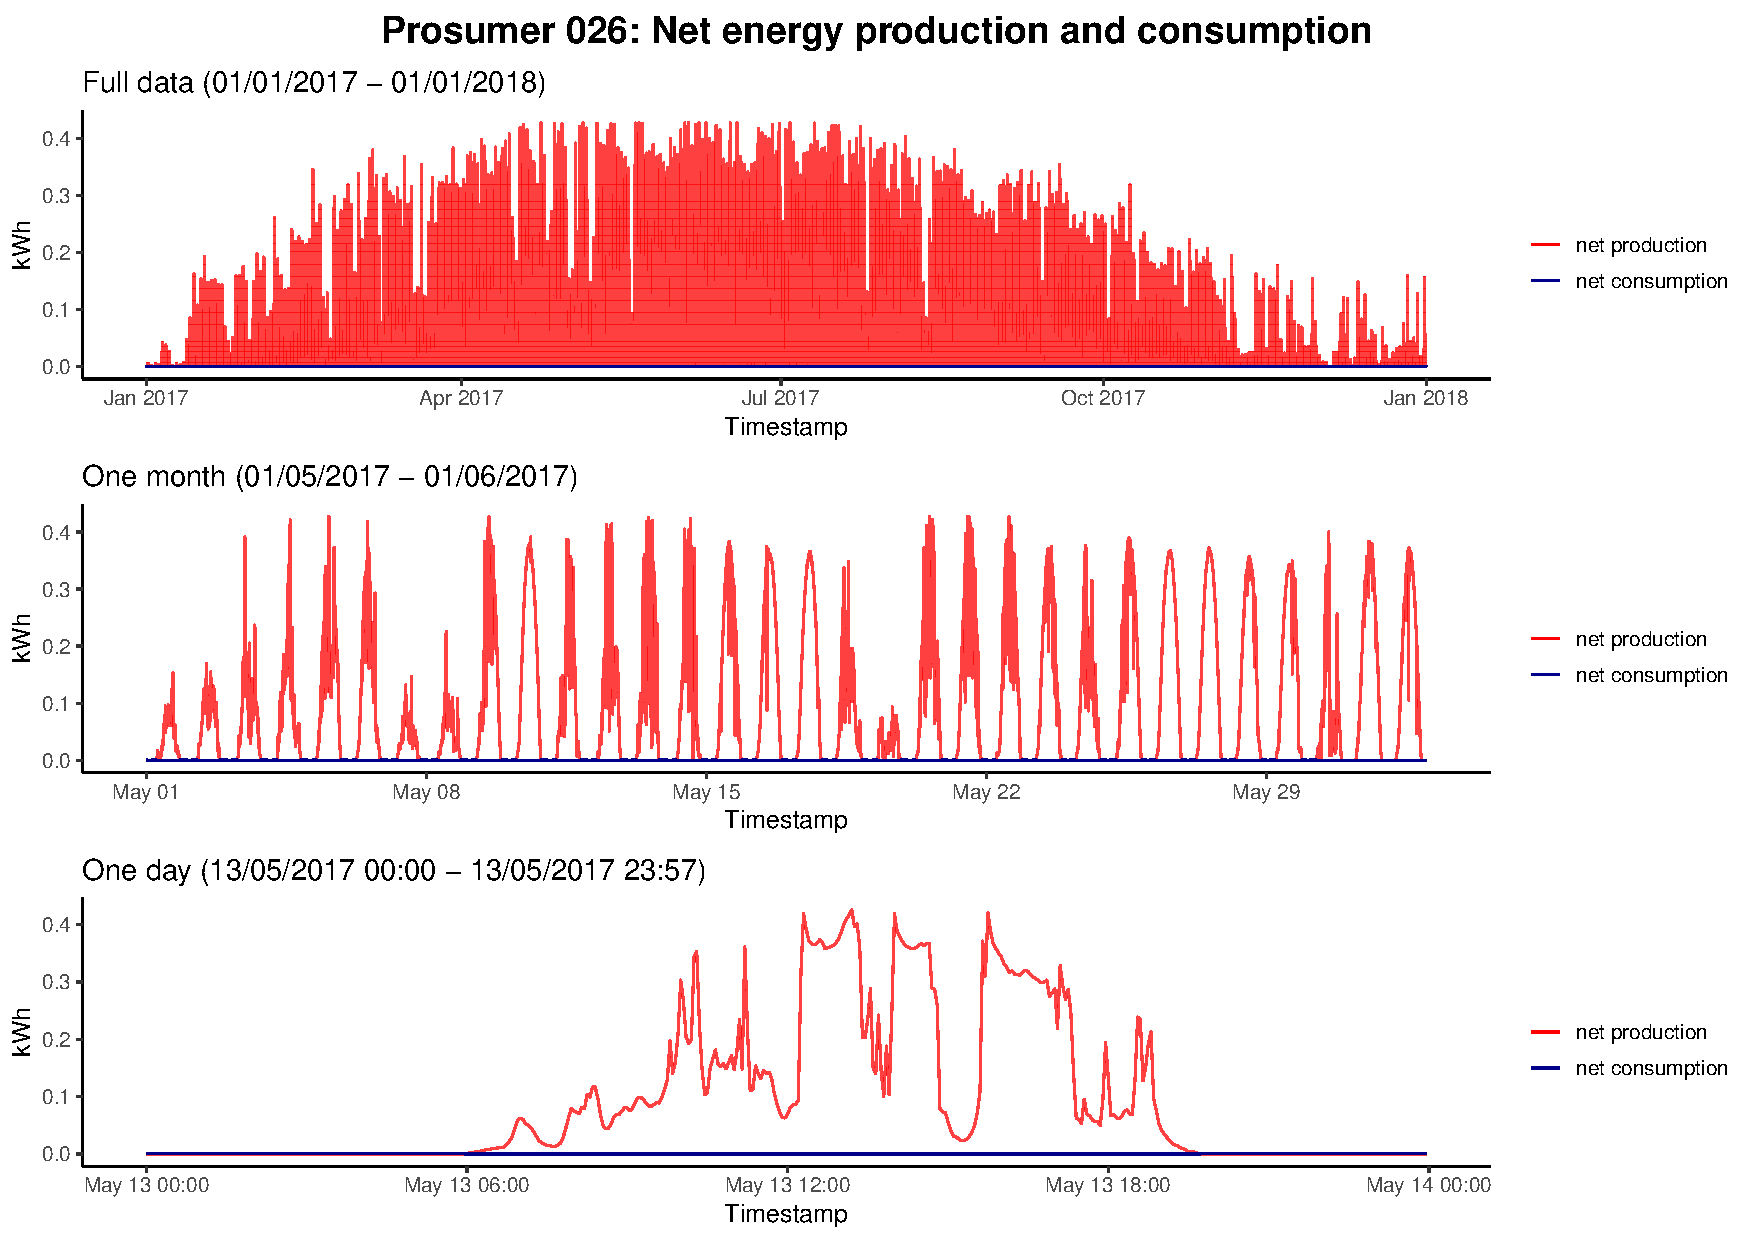
\includegraphics[width=\textwidth]{thesis/graphs/timeseries/p026_prod&cons.pdf}
\end{minipage}
\begin{minipage}[h]{\dimexpr.5\textheight-0.15em}
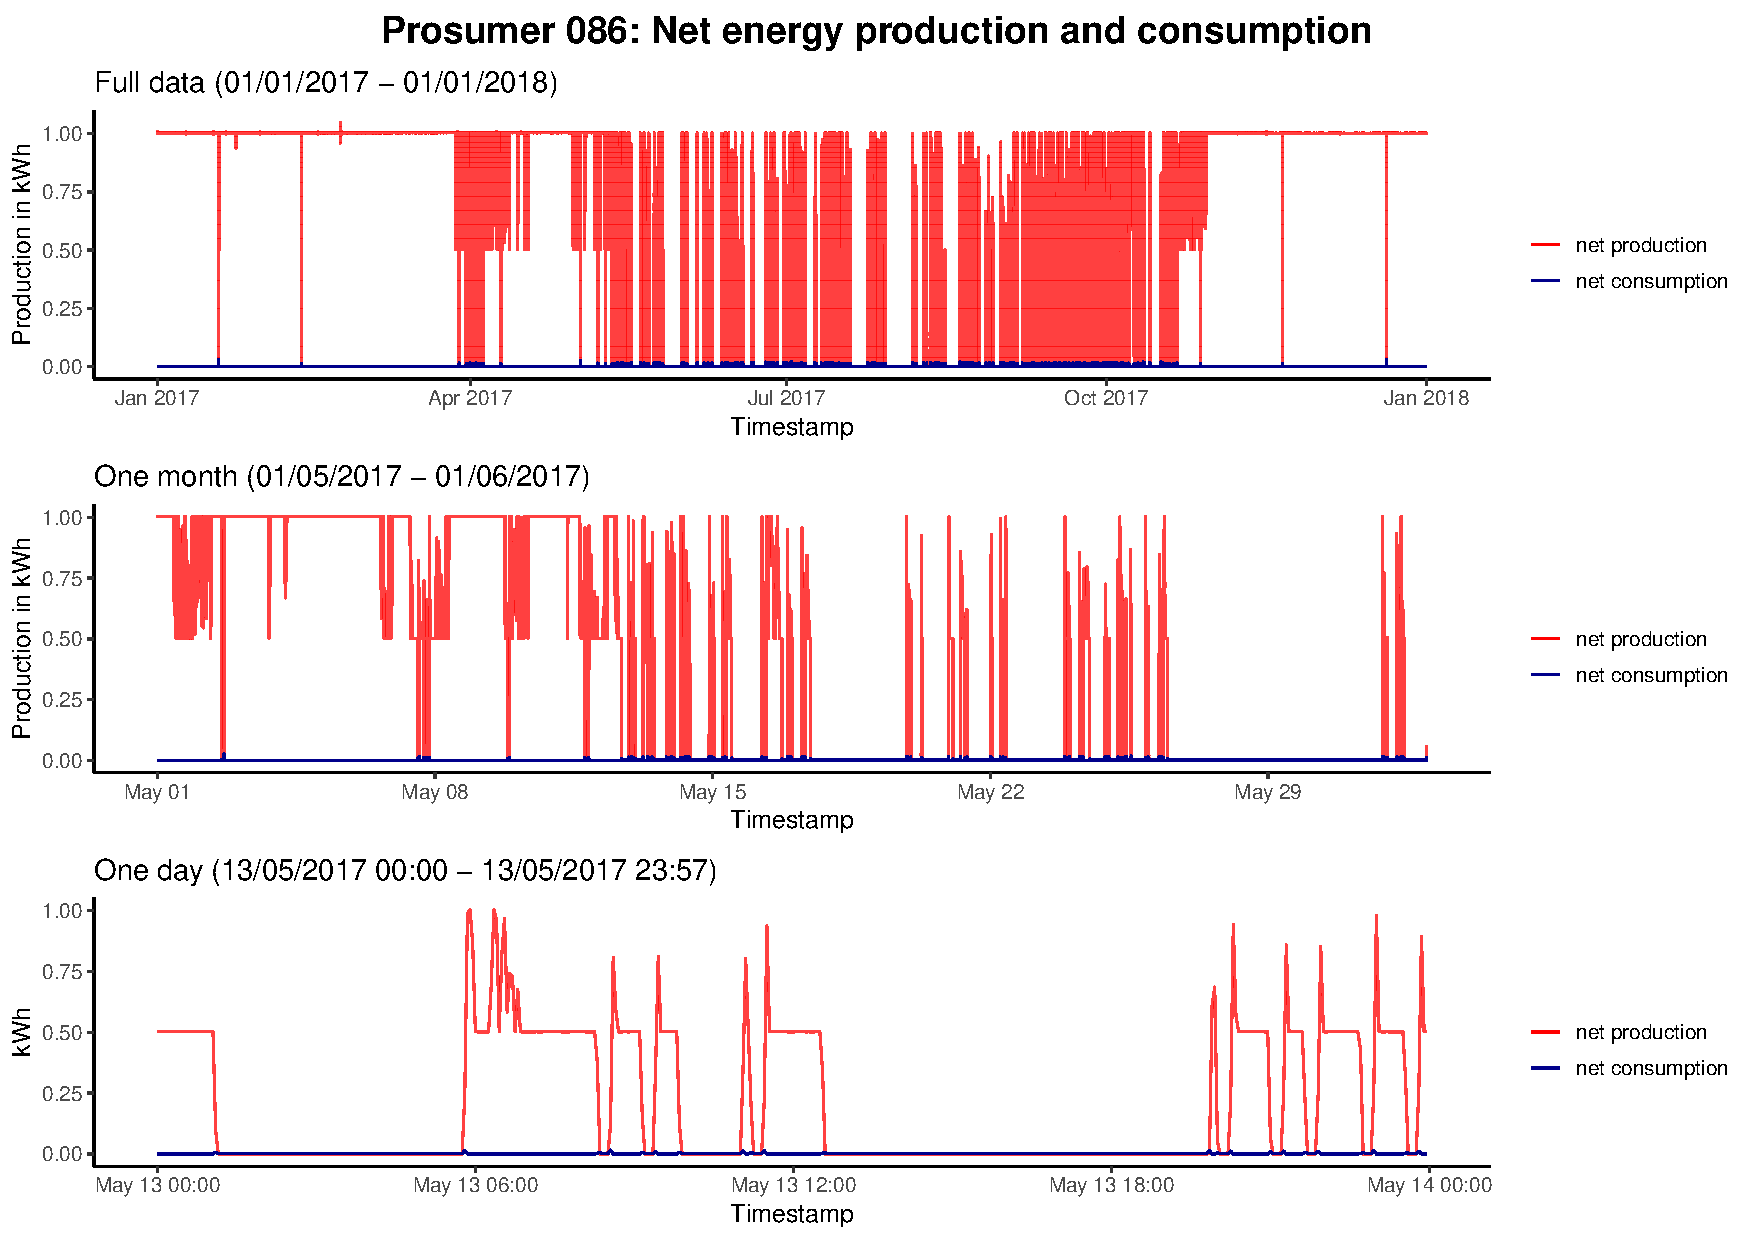
\includegraphics[width=\textwidth]{thesis/graphs/timeseries/p086_prod&cons.pdf}
\end{minipage}

\caption[Energy consumption and production recordings of prosumer~026 and 086]{Energy consumption and production recordings of prosumer~026 and 086. The first panel in the respective graph shows the full year 2017, the second panel zooms in to one month (May), and the third panel zooms in to one day (May, 13). \quantnet\href{https://github.com/QuantLet/BLEM/tree/master/BLEMplotEnergyData}{BLEMplotEnergyData}}
\label{Fig:energyconsprod_p026p086}

\end{sidewaysfigure}
%
A plausible explanation for the kind of net production pattern exhibited by prosumer~086 may be a combined heat and power unit (CHP) (also known as block-type thermal power station or BTTP). This assumption also supported by the increasing frequency of drops in net energy production over the summer months. In these months much less heating is needed resulting in more downtime of the CHP and therefore also more periods of zero net energy production. However, as mentioned in the discussion of the consumer data sets, unfortunately, there is no additional context information available for the data sets at hand making this kind of assumption purely speculative.

In conclusion, it becomes clear that the prosumers' net energy consumption and production follow much less easily explainable patterns. The net energy consumption is much more heterogeneous. Additionally, most prosumer data sets do not contain any recordings of net energy production at all. Of those prosumers that do have positive net production values, most surpass the energy consumption of a typical household with their net energy production by far. Implications of this for the suitability of the data sets for the prediction task at hand will be discussed in Section~\ref{Sec:Data;Subsec:Exclusion}.



%%%%%%%%%%%%%%%%%%%%%%%%%%%%%%%%%%%%%
%%%   Peculiarities in the data   %%%
%%%%%%%%%%%%%%%%%%%%%%%%%%%%%%%%%%%%%

\subsection{Peculiarities in the data}\label{Sec:Data;Subsec:Peculiarities}



%%%%%%%%%%%
\subsubsection{Consumer data sets}

The data sets were analyzed for peculiarities in the time series patterns that seemed to be systematically different than the majority of data sets. One such peculiarity is the occurrence of zero values. In any household that does not produce its own energy (pure consumer household), energy consumption of 0 kWh, even only for a very short period of time, seems to be very unlikely (apart from the rare case of a power outage in the area or when the main switch of the household is turned off). Thus, it is not surprising that 93~\% of the data sets do not contain any 0 kWh measurements per 3-minute interval at all. Of the remaining 6 data sets, one contains just a single measurement of 0 kWh, which seems plausible. The other data set with a small amount of zero values is consumer~082 which was discussed in detail in Section~\ref{Sec:Data;Subsec:Description}. In Figure~\ref{Fig:energycons_c082} showing consumer~082's consumption values, it is visible that although the consumption pattern does not change substantially, the lowest values of the daily fluctuations are lower in the second half of 2017 than in the first half. However, this seems still a plausible consumption pattern for a typical household. The other five data sets, on the contrary, contain between 34 and 54~\% of zero values. Examining the consumption time series more closely also reveals, that these households exhibit a systematically different consumption pattern that one would expect from a typical household.

\begin{sidewaysfigure}[htbp]
    \centering
    \begin{minipage}[ht]{\dimexpr.5\textheight-0.15em}
    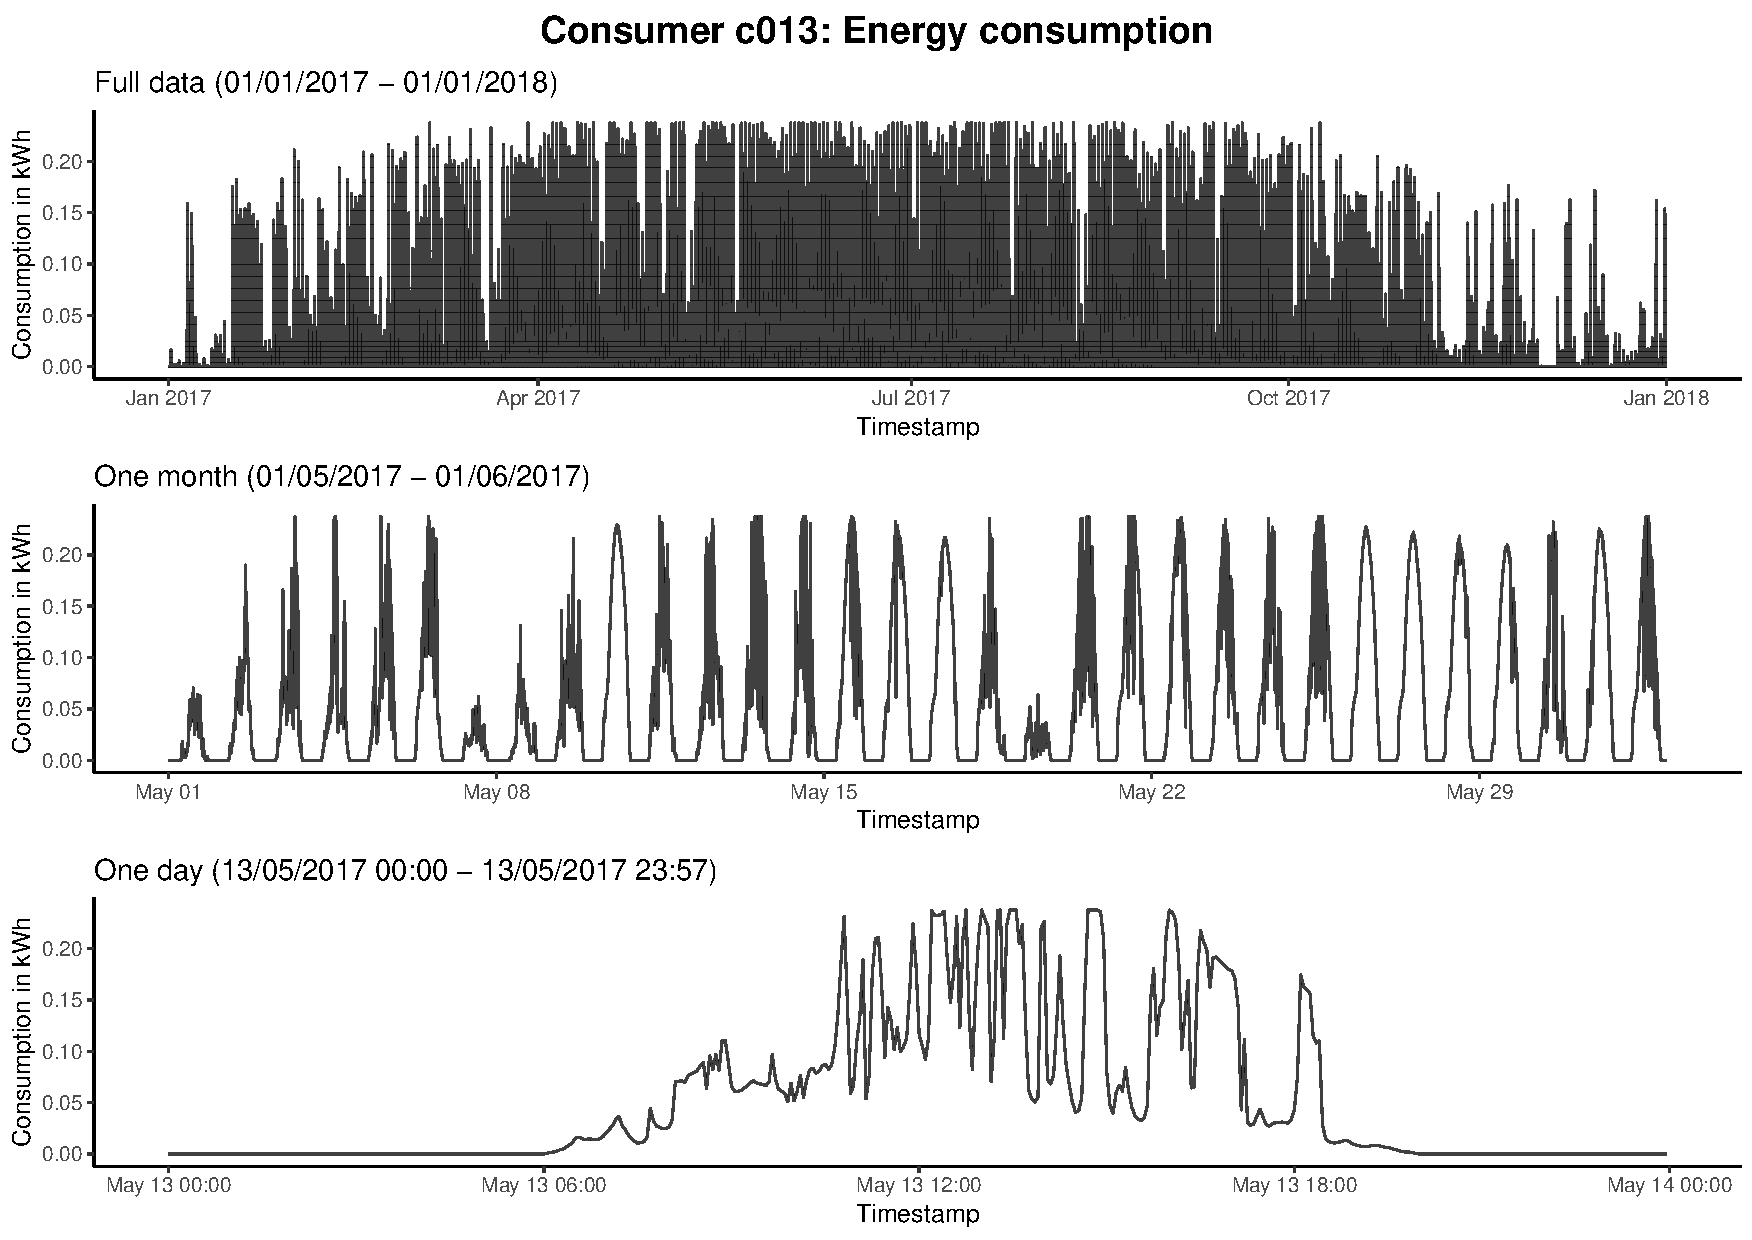
\includegraphics[width=\textwidth]{thesis/graphs/timeseries/c013_cons.pdf}
    \end{minipage}
    \begin{minipage}[ht]{\dimexpr.5\textheight-0.15em}
    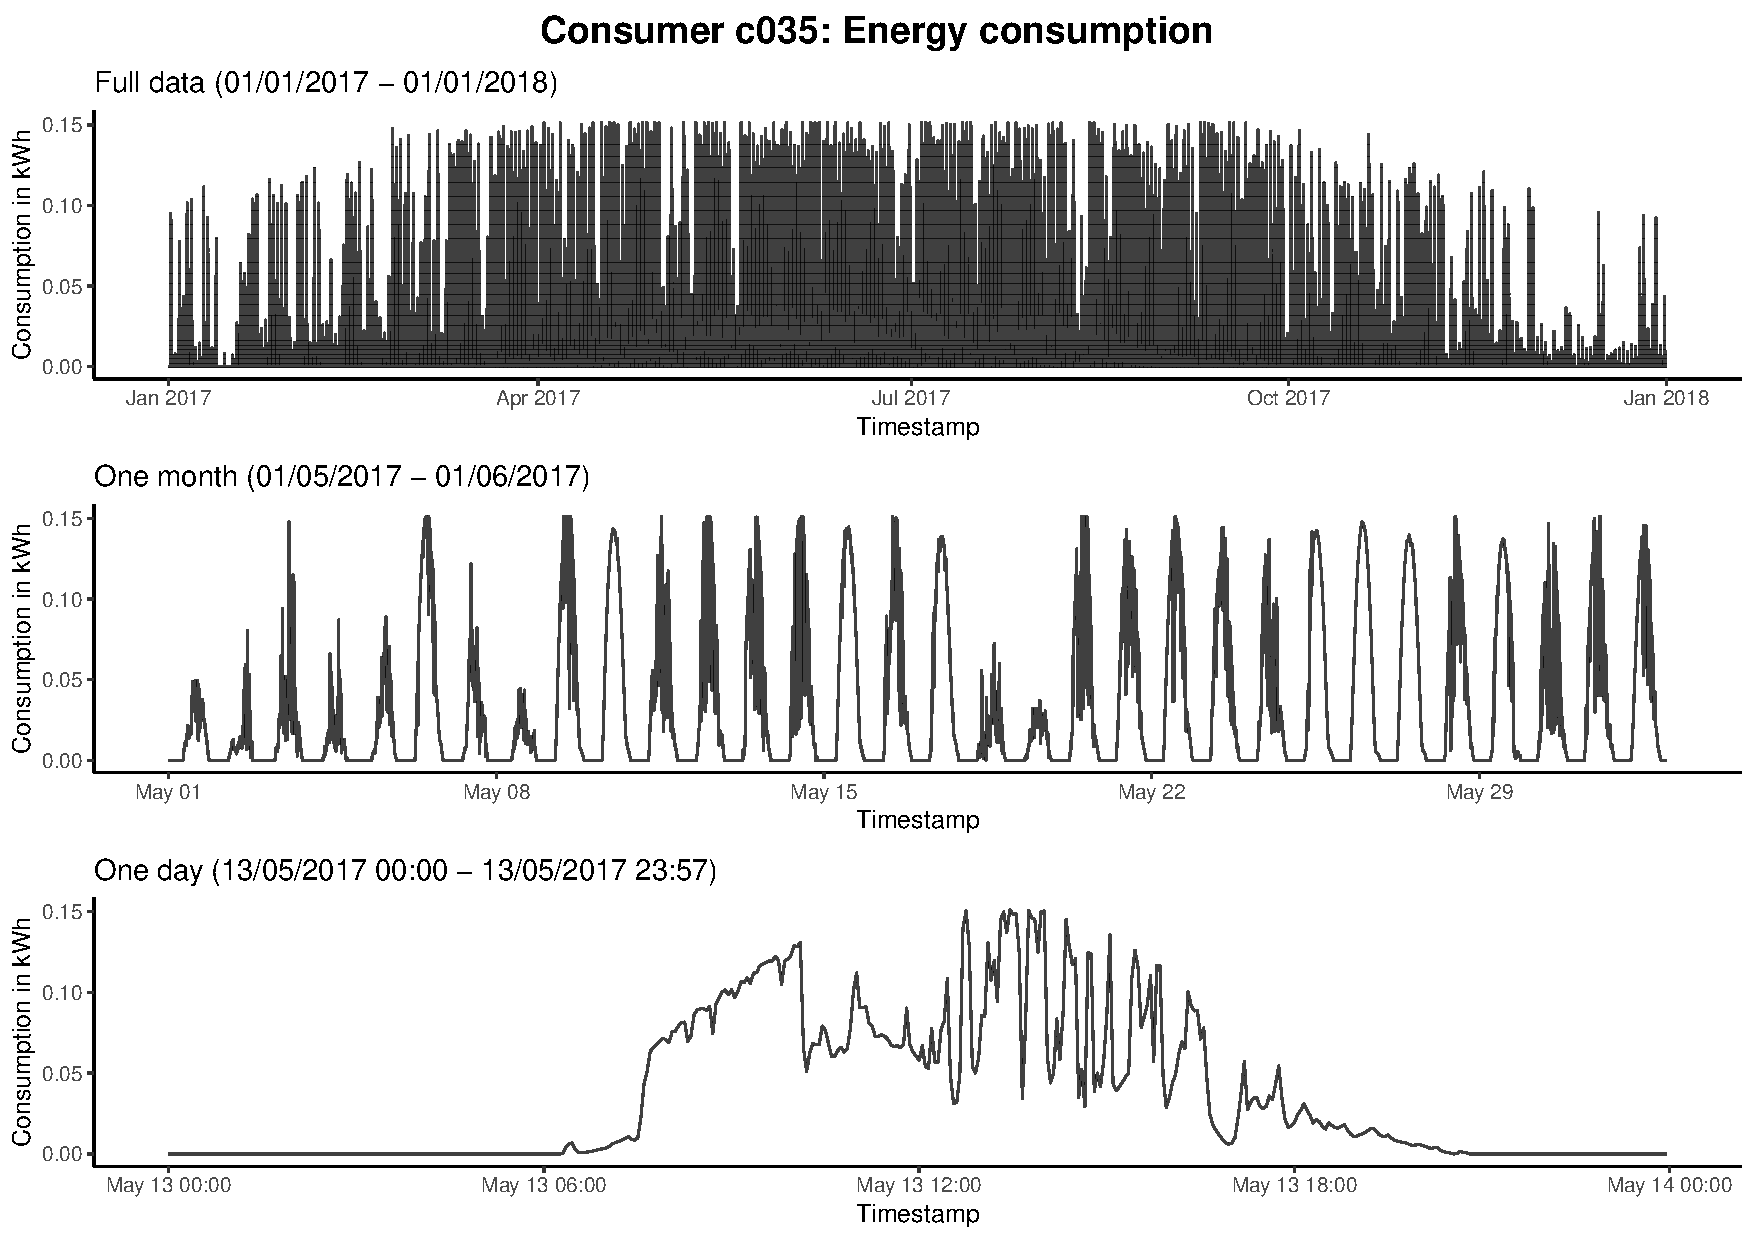
\includegraphics[width=\textwidth]{thesis/graphs/timeseries/c035_cons.pdf}
    \end{minipage}\\
    
    \begin{minipage}[ht]{\dimexpr.5\textheight-0.15em}
    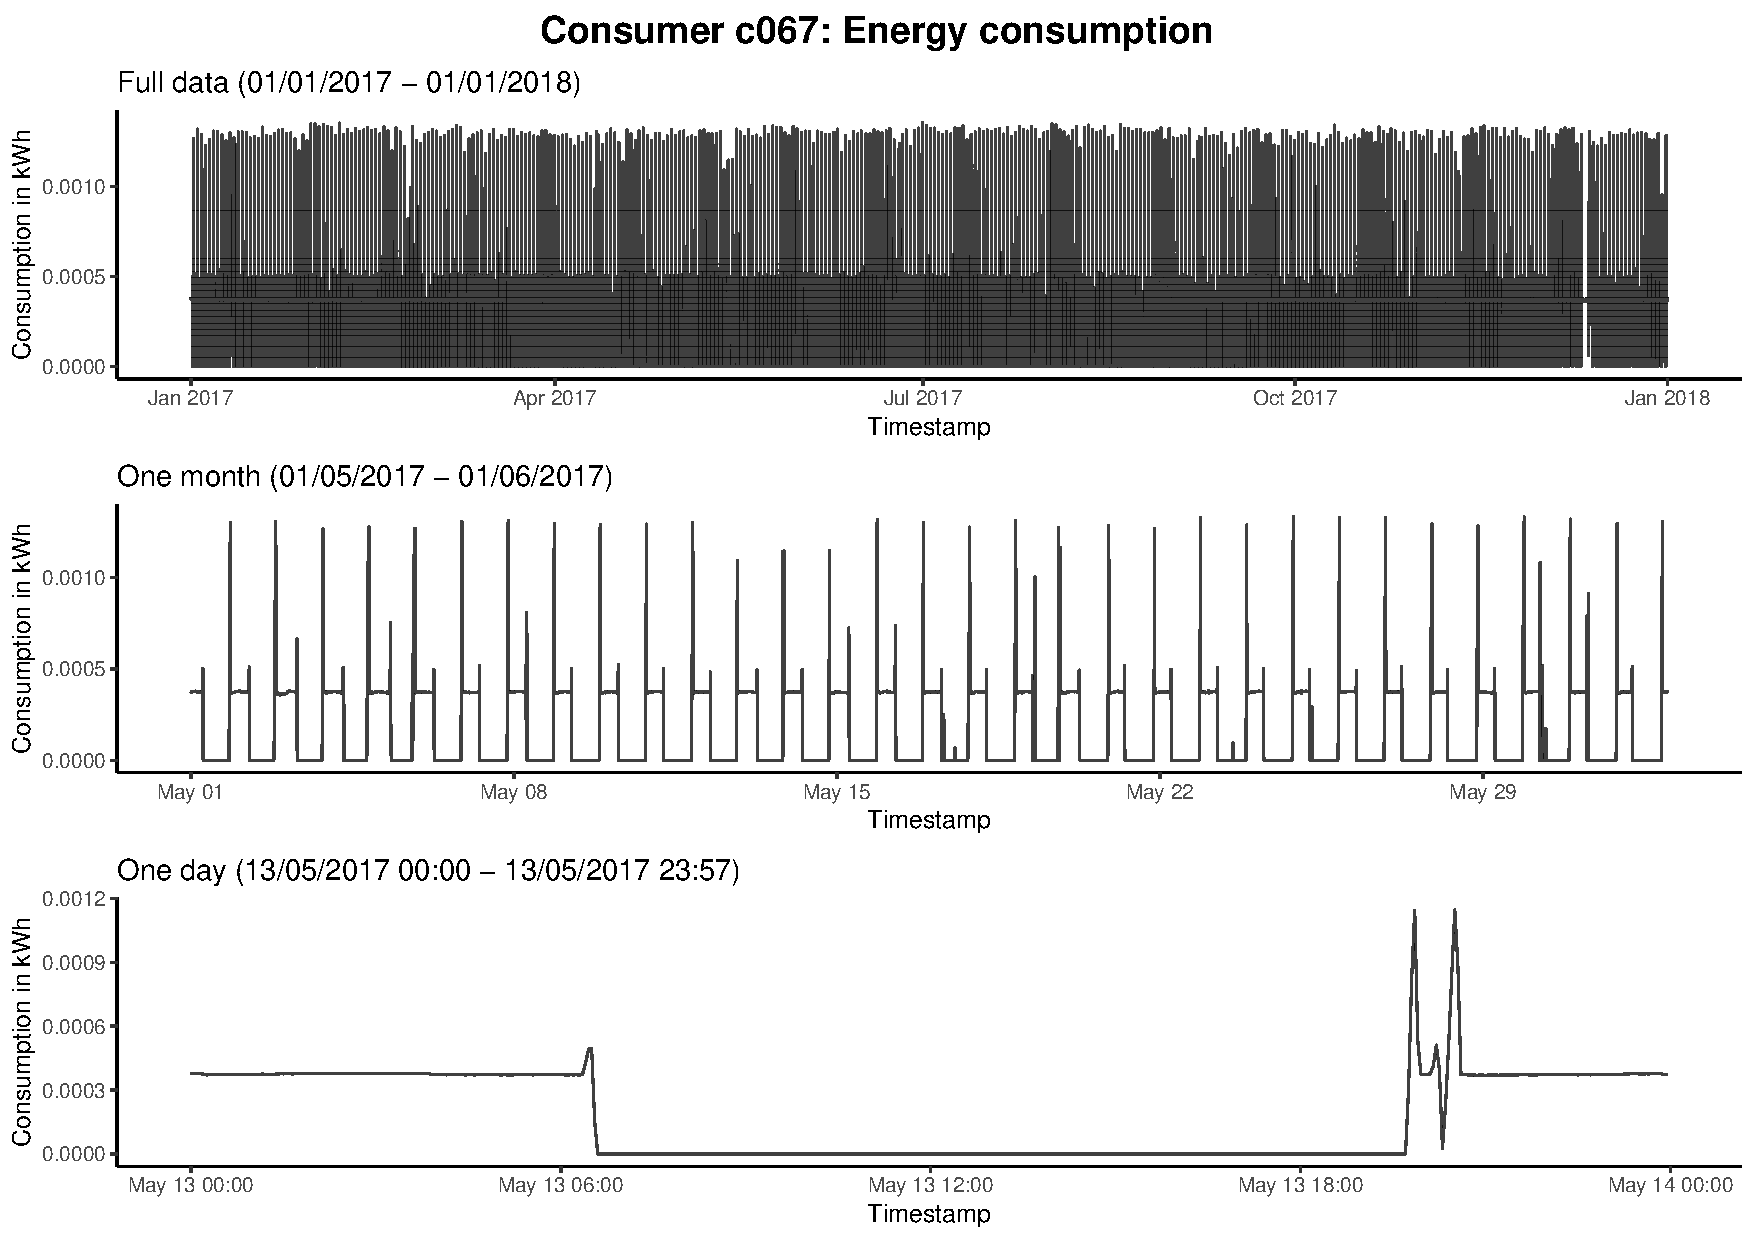
\includegraphics[width=\textwidth]{thesis/graphs/timeseries/c067_cons.pdf}
    \end{minipage}
    \begin{minipage}[ht]{\dimexpr.5\textheight-0.15em}
    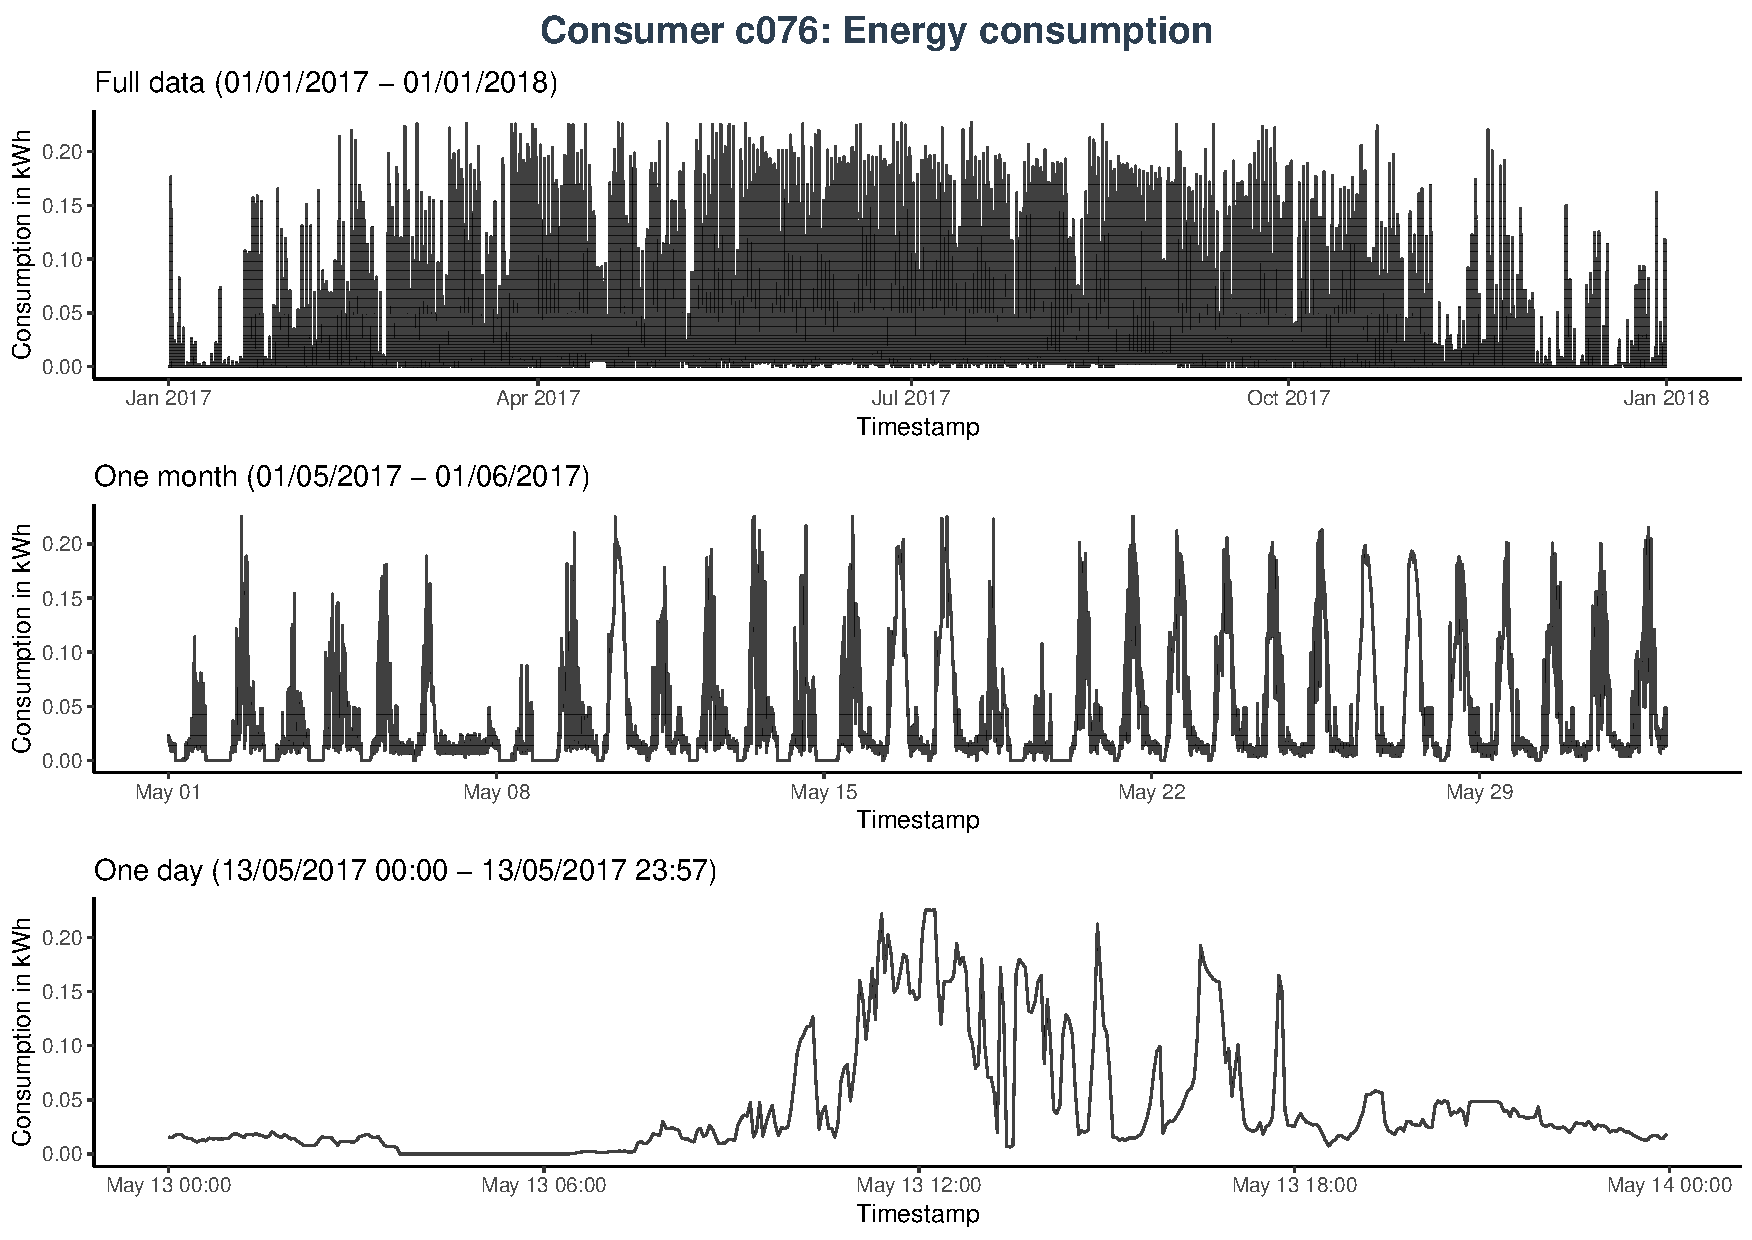
\includegraphics[width=\textwidth]{thesis/graphs/timeseries/c076_cons.pdf}
    \end{minipage}
    
    \caption[Energy consumption of consumers with conspicuous consumption patterns]{Energy consumption recordings of consumers with conspicuous consumption patterns. \quantnet\href{https://github.com/QuantLet/BLEM/tree/master/BLEMplotEnergyData}{BLEMplotEnergyData}}
    \label{Fig:consenergycons_peculiar}
\end{sidewaysfigure}

Figure~\ref{Fig:consenergycons_peculiar} shows the time series of the aforementioned four consumers with a high share of zero measurements. Consumer~013 and 035 both show a very similar pattern of daily energy consumption. Looking at the middle panel of the two upper graphs in Figure~\ref{Fig:consenergycons_peculiar}, the regularity of the consumption increases and decreases for each day is striking. The lower panel shows again, exemplary, May 13, 2017. Energy consumption starts to (almost linearly) increase at about 6 a.m.~and decreases to 0 kWh at about 6 p.m. ~This also explains the 52.77~\% and 54.02~\% of zero values in those to data sets: almost exactly 12 hours per day (from midnight to 6 a.m.~and from 6 p.m.~to midnight) the consumption is zero, while the energy consumption fluctuates in the meantime with a relatively high ``base" consumption. Switching back to the middle panel, it is noticeable that there are some days in May with an even smoother energy consumption increase and decrease over the course of the day. As there is no further socio-demographic data available, we can only guess what the reason for such different consumption patterns are. The most likely explanation seems to be, that the consumption time series of consumer~013 and 035 belong to small businesses rather than to a households.

The lower two graphs of Figure~\ref{Fig:consenergycons_peculiar} show the energy consumption time series of consumer~067 and consumer~076. Consumer~067's consumption pattern zoomed in to one month (middle panel) rather looks like an electrocardiogram than what one would expect from a household energy consumption time series. The regularity of amplitude and frequency is obvious but not easily explained. Consumers~076's consumption pattern looks less suspicious at first sight. However, closer inspection reveals the same daily pattern of increasing consumption throughout the day and very low to zero energy consumption at night. This again rather resembles the energy consumption pattern of a business building or office rooms than a typical household.



%%%%%%%%%%%
\subsubsection{Prosumer data sets}

For prosumers, peculiarities in the time series pattern can be found either in the net energy consumption or net energy production or in combination. As net energy consumption is much more heterogeneous in the prosumer data sets than in the consumer data sets, it is less obvious what patterns fall outside the norm. However, some prosumer still exhibit obvious anomalies in their consumption patterns. Prosumer~046, 061, and 079 stand out as their consumption is zero for the largest part of the year. This would be an expected pattern if they were net energy producers during this time period. However, as they do not feed in any produced energy at all in 2017, this consumption pattern indicates a data problem. 
Prosumer~038 attracts attention by having a very low total net energy consumption of just 18 kWh in 2017 and zero net production. Moreover, this energy is consumed at an extremely low level of around 0.0001 kWh with a standard deviation of $\sigma=2\times10^{-6}$ and just one single drop from this level to zero in the whole year (see Figure~\ref{Fig:energycons_p038}). Six more prosumers exhibit a similar pattern of stable level of net energy consumption with occasional drops to zero but no spikes above this stable level. None of them is a net energy producer at any time.

\begin{figure}[htbp]
 \centering
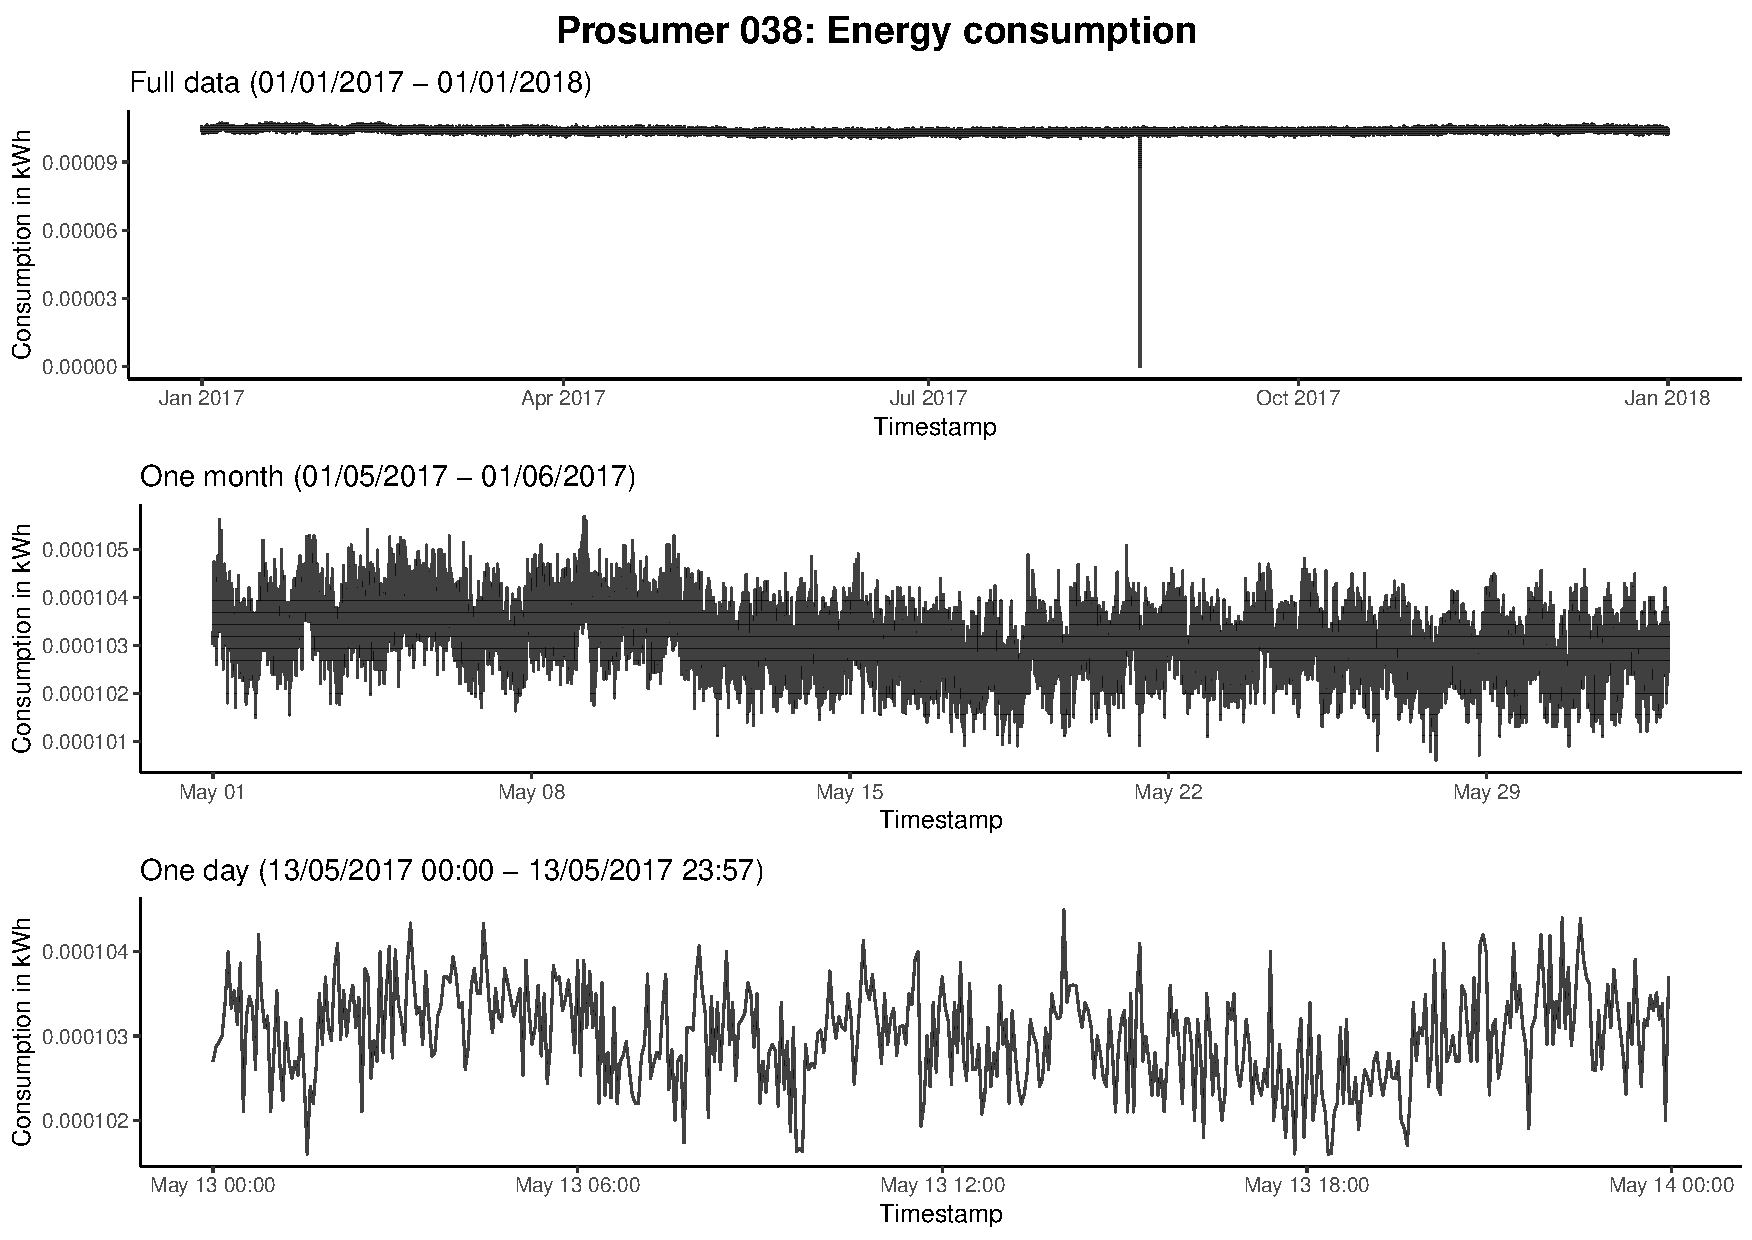
\includegraphics[width=\textwidth]{thesis/graphs/timeseries/p038_cons.pdf}
\caption[Energy consumption recordings of prosumer 038]{Energy consumption recordings of prosumer~038. The first panel shows the full year 2017, the second panel zooms in to one month (May), and the third panel zooms in to one day (May, 13). \quantnet\href{https://github.com/QuantLet/BLEM/tree/master/BLEMplotEnergyData}{BLEMplotEnergyData}}
\label{Fig:energycons_p038}
\end{figure}

Lastly, prosumer~019 is worth mentioning as it is the only prosumer data set that records a total net energy consumption of 0 kWh for 2017. As the net energy production, however, contains a substantial amount of zero values as well, it seems implausible that prosumer 019 is a regular household. For a household, it appears unlikely that the energy consumption is always zero when the energy production is zero as well.

Regarding the production time series, most of the prosumer data sets are peculiar in so far as they have only zero net production values. It seems at least somewhat unlikely that a majority of households equipped with energy production capacities consumes more than it produces over the whole course of the year at any point in time. However, it is unfortunately not possible to get feedback from Discovergy due to privacy and internal policy reasons on why 84 out of 100 prosumer data sets do not record any electricity fed into the grid at all.

\begin{sidewaysfigure}[htbp]
\centering
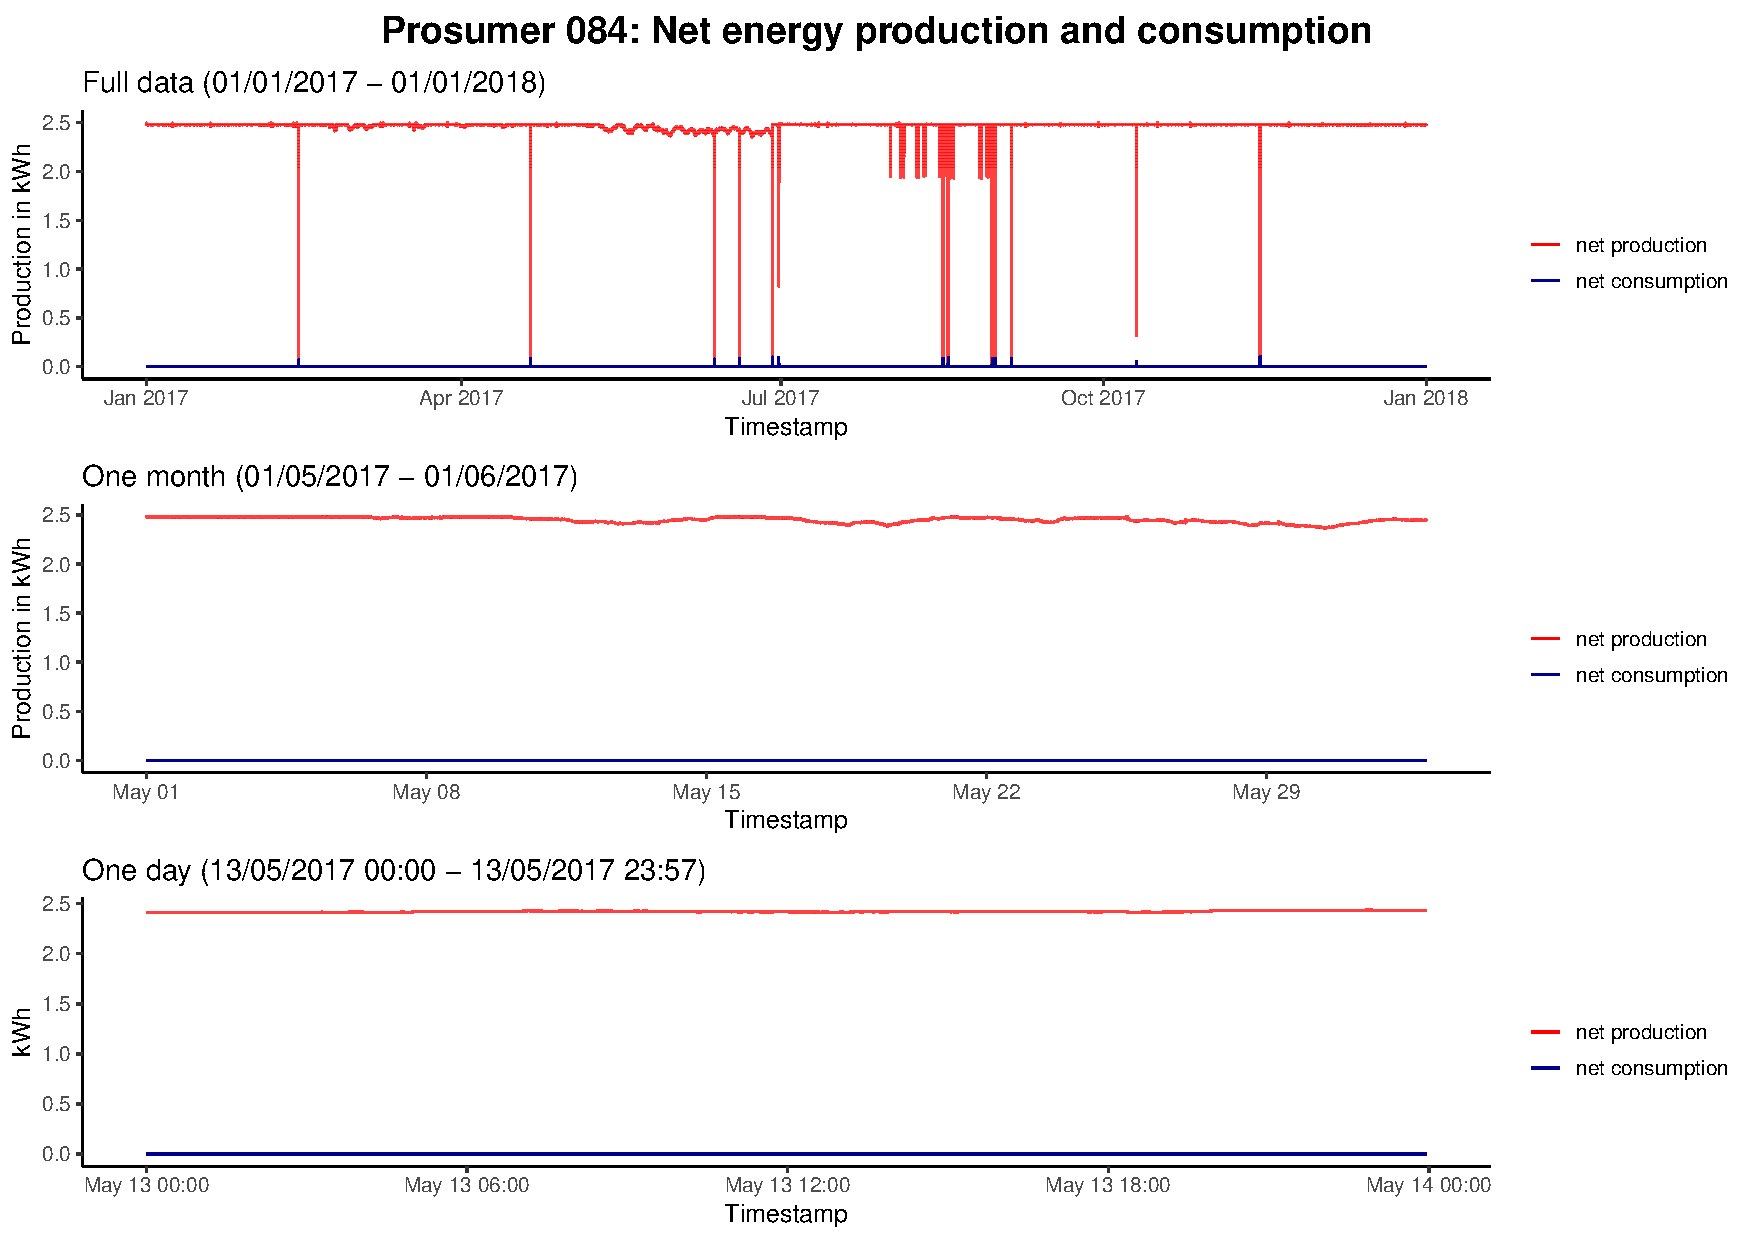
\includegraphics[width=.5\textwidth-0.15em]{thesis/graphs/timeseries/p084_prod&cons.pdf}
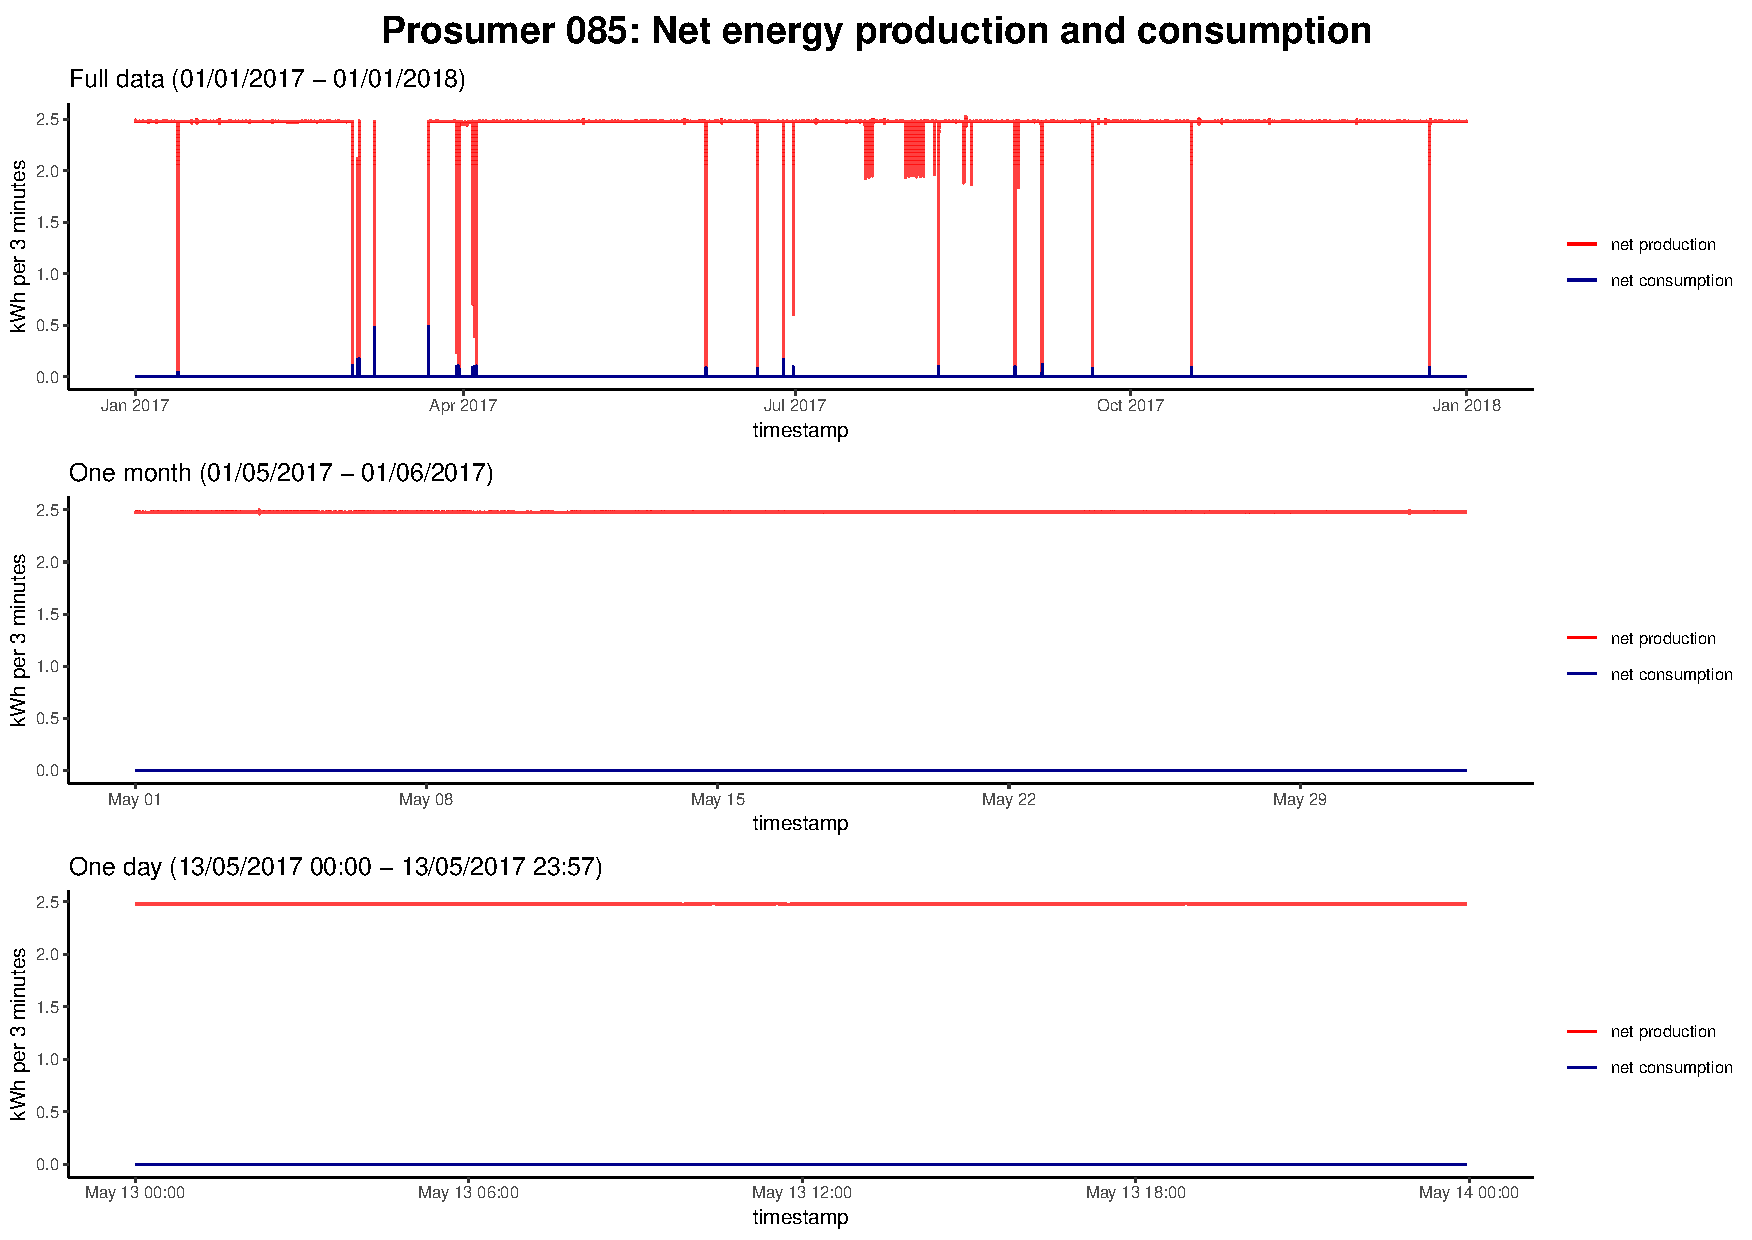
\includegraphics[width=.5\textwidth-0.15em]{thesis/graphs/timeseries/p085_prod&cons.pdf}

\caption[Energy consumption and production recordings of prosumer 084 and 085]{Energy consumption and production recordings of prosumer~024 and 085. The first panel in the respective graph shows the full year 2017, the second panel zooms in to one month (May), and the third panel zooms in to one day (May, 13). \quantnet\href{https://github.com/QuantLet/BLEM/tree/master/BLEMplotEnergyData}{BLEMplotEnergyData}}
\label{Fig:energyconsprod_p084p085}
\end{sidewaysfigure}

Of the remaining 14 data sets, prosumer 084 and 085 stand out as their net energy production time series is almost a flat line at 2.5 kWh per 3-minute interval. Their graphs are shown in Figure~\ref{Fig:energyconsprod_p084p085}.

In conclusion, it seems like the majority of prosumer data sets with non-zero net production values were recorded by smart meters that just record the energy production of a certain installation and not of a household with production capacity. This is not per se a problem, as these installations can act as a individual agent on a local energy market. Even though, they might belong to a household with a separate smart meter, they can sell energy through their own smart meter while the related household's smart meter buys energy. If both smart meters are connected to the same blockchain wallet, this automatically solves the challenge of pricing the energy relative to the own consumption.



%%%%%%%%%%%%%%%%%%%%%%%%%%%%%%
%%%   Data sets excluded   %%%
%%%%%%%%%%%%%%%%%%%%%%%%%%%%%%

\subsection{Data sets excluded}\label{Sec:Data;Subsec:Exclusion}
The data sets of consumer~013, 035, 067 and 076 shown in Figure~\ref{Fig:consenergycons_peculiar} where excluded from the prediction task for the reasons discussed in Section~\ref{Sec:Data;Subsec:Peculiarities}. These four consumers plus one additional consumer (consumer~082) exhibited non-negligible shares of zero consumption values leading to their exclusion. Further, consumer~046 was excluded as the consumption time series was flat for the most part of 2017. After some initial fluctuations in the first quarter, all fluctuations stopped entirely. Four more consumers were excluded due to conspicuous regularity in daily or weekly consumption patterns. Lastly, consumer~080 was excluded due to very low and stable consumption values with very rare, extreme spikes. The time series graphs of all additionally to the ones shown in Figure~\ref{Fig:consenergycons_peculiar} excluded consumer data sets are shown in Appendix~\hyperlink{AppA1:Figures:Excludedc}{A1}. Consumer~026 was excluded not due to peculiarities in the consumption patterns but due to missing data. For some unknown reason, the last recorded measurement for consumer~026 is 2017-12-29~07:03:00. As the inclusion of this shorter time series would lead to difficulties in the forecasting algorithms, this data set was excluded as well.

Out of the 100 prosumer data sets, 86 were excluded from the prediction task due to zero total net energy production in 2017. These ``prosumers" would not act as prosumers in a local energy market as they never actually supply a production surplus to the market. Moreover, as their net energy production is always zero, their net energy production shows no variation which is a necessary precondition to train any prediction model.

Of the remaining 14 prosumer data sets, prosumer 012 was excluded as the total net energy it fed into the grid in 2017 was just 22 kWh. Even though, the feed in occurred continuously over the whole year, it never exceeded 0.0013 kWh per 3-minute interval with a mean of 0.0001 kWh, which is too small to be relevant. Prosumer 015 was excluded as it only fed energy into the grid in the period from 06.01.2017 to 19.01.2017. For all other measurement points the net energy production was zero. The time series graph of the two excluded prosumer data sets with production data are shown in Appendix~\hyperlink{AppA2:Figures:Excludedp}{A2}.

Hence, 88 consumer and 12 prosumer data sets remained for the prediction tasks. All data sets included a time stamp and the consumption time series for consumers respectively the production time series for prosumers with a total of 175,200 data points each.

%%%%%%%%%%%%%%%%%%%%%%%%%%%%%%%%%%%%%%%%%%%%%%%%%%%%%%%%%%%%%%%%%

\newpage
\section{Results}\label{Sec:Results}

The results are presented in three parts that correspond to the three research questions put forward in Section~\ref{Sec:Intro;Subsec:Present}: First, the forecasting accuracy of the prediction models is evaluated and reported. Second, the results of the market simulation -- which was run once with the true consumption and production values and once with predicted consumption values in three different supply scenarios -- are presented. Third, the implications of the results of the market simulation are discussed.


%%%%%%%%%%%%%%%%%%%%%%%%%%%%
%%%   Benchmark models   %%%
%%%%%%%%%%%%%%%%%%%%%%%%%%%%

\subsection{Evaluation of the prediction models}\label{Sec:Results;Subsec:Forecast}

Three prediction methods were used to forecast the energy consumption of 88 consumer households and to forecast the energy production of 12 prosumer households 15 minutes ahead: a benchmark model (see Section~\ref{Sec:Method;Subsec:Benchmark}), a LSTM RNN model (see Section~\ref{Sec:Method;Subsec:LSTM}), and a LASSO model (see Section~\ref{Sec:Method;Subsec:LASSO}). All three prediction models were compared and evaluated using the error measures presented in Section~\ref{Sec:Method;Subsec:Error}.


%%%%%%%%%%%
\subsubsection{Consumption data}

The performance of the prediction models was tested on a quarter of the available data. That is, the prediction models were fitted on the consumption values from 01.01.2017~00:00 to 30.09.2017~00:00 which is equivalent to 131,040 data points per data set. For all 88 consumer data sets, the models were fitted separately resulting in as many distinct LASSO and LSTM prediction models. The fitted models were then used to make energy consumption predictions in 15-minutes intervals for each household individually on the data from 01.10.2017~00:00 to 01.01.2018~00:00. This equates to 8,836 predicted values per data set per prediction method.

Figure~\ref{Fig:glimpse_predcons} exemplary shows the true and predicted consumption values of consumer~011 on October 27, 2017. The na\"ive benchmark model just follows the true consumption shifted by one time step (i.e., 15 minutes). This fits the true values generally good, as long as there are no sudden jumps in the household's energy consumption. Spikes in energy consumption, as in this example one occurred in the 15 minutes before 07:30 a.m.~and 08.30 a.m.~respectively, necessarily lead to two periods with high errors of the na\"ive predictor: First, once the jump to a high consumption level occurs and the na\"ive predictor remains at the previous low level, and second, once the consumption suddenly returns to the low consumption level and the na\"ive predictor persists at the high level of the previous period. In such situations, the LASSO and LSTM models are more accurate. Even though they underestimate the jumps in energy consumption, they do not lag behind as much as the na\"ive predictor and, generally, have the ability to anticipate movements. However, the exemplary glimpse onto the predicted consumption values of consumer~011 already reveals that also the sophisticated prediction models lack the ability to accurately predict sudden movements in the energy consumption and tend to overestimate low consumption levels and underestimate spikes in energy consumption.
%
\begin{figure}[htbp]
    \centering
    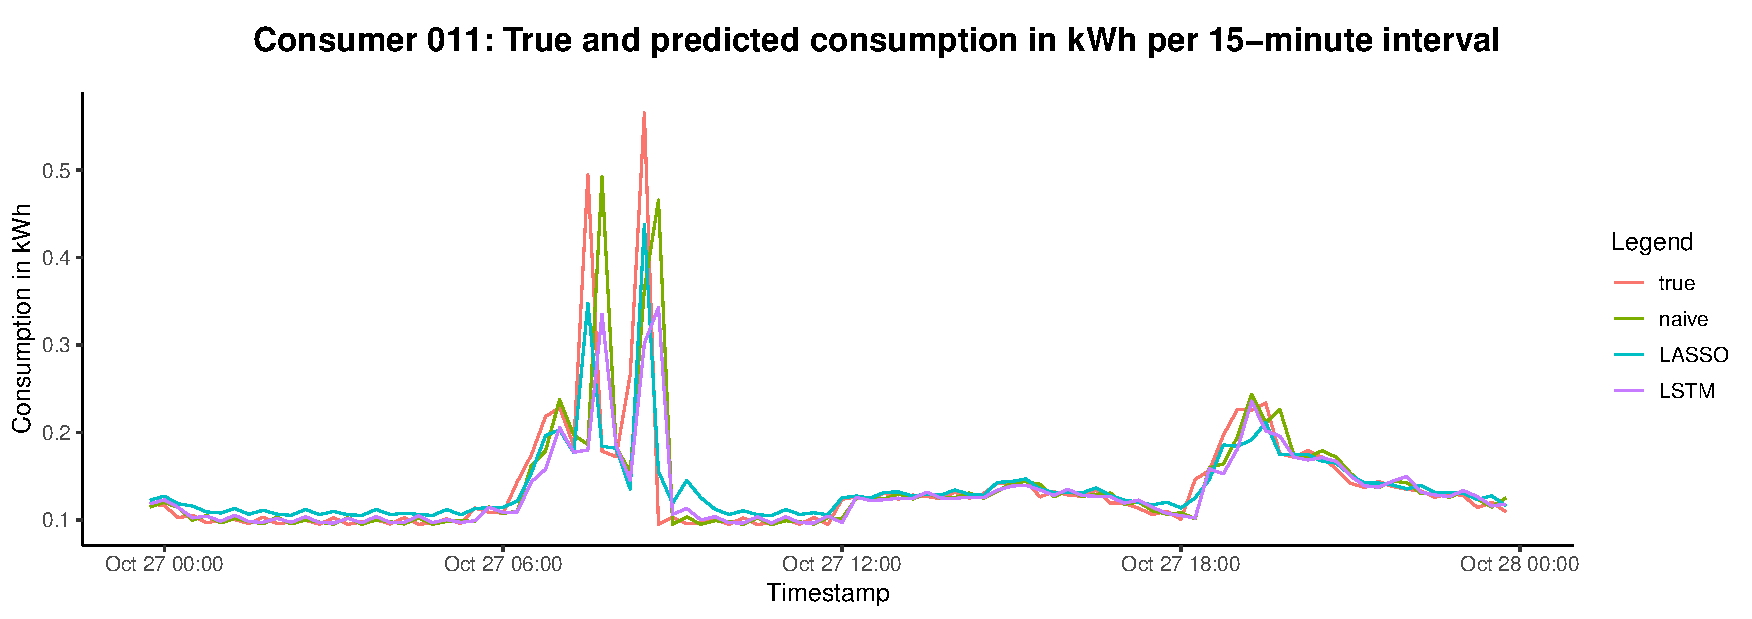
\includegraphics[width=\textwidth]{thesis/graphs/evaluation/c011_pred_cons.pdf}
    \caption[Exemplary 24 hours of true and predicted consumption values]{Exemplary 24 hours of true and predicted consumption values of consumer 011. \quantnet\href{https://github.com/QuantLet/BLEM/tree/master/BLEMplotEnergyPreds}{BLEMplotEnergyPreds}}
    \label{Fig:glimpse_predcons}
\end{figure}
%

Systematically analyzing the total over- and underestimation of the different prediction models on each consumer data set confirms this impression. Figure~\ref{Fig:overunderestimation} displays the total sum of over- and underestimation errors of each prediction method per data set. As one would expect, the na\"ive benchmark model consistently over- and underestimated by the same amount per data set. The reason for that is that the sum of over- and underestimation errors only depends on the amplitude of the spikes in energy consumption. Thus, overestimation errors occur in the same frequency and magnitude as underestimation errors. The LASSO model achieved overall lower total sums of errors than the benchmark model. Notably, the sum of underestimation errors is higher across the data sets than the sum of overestimation errors. This points towards a general tendency of underestimating sudden increases in energy consumption by the LASSO model.
%
\begin{figure}[!ht]
    \centering
    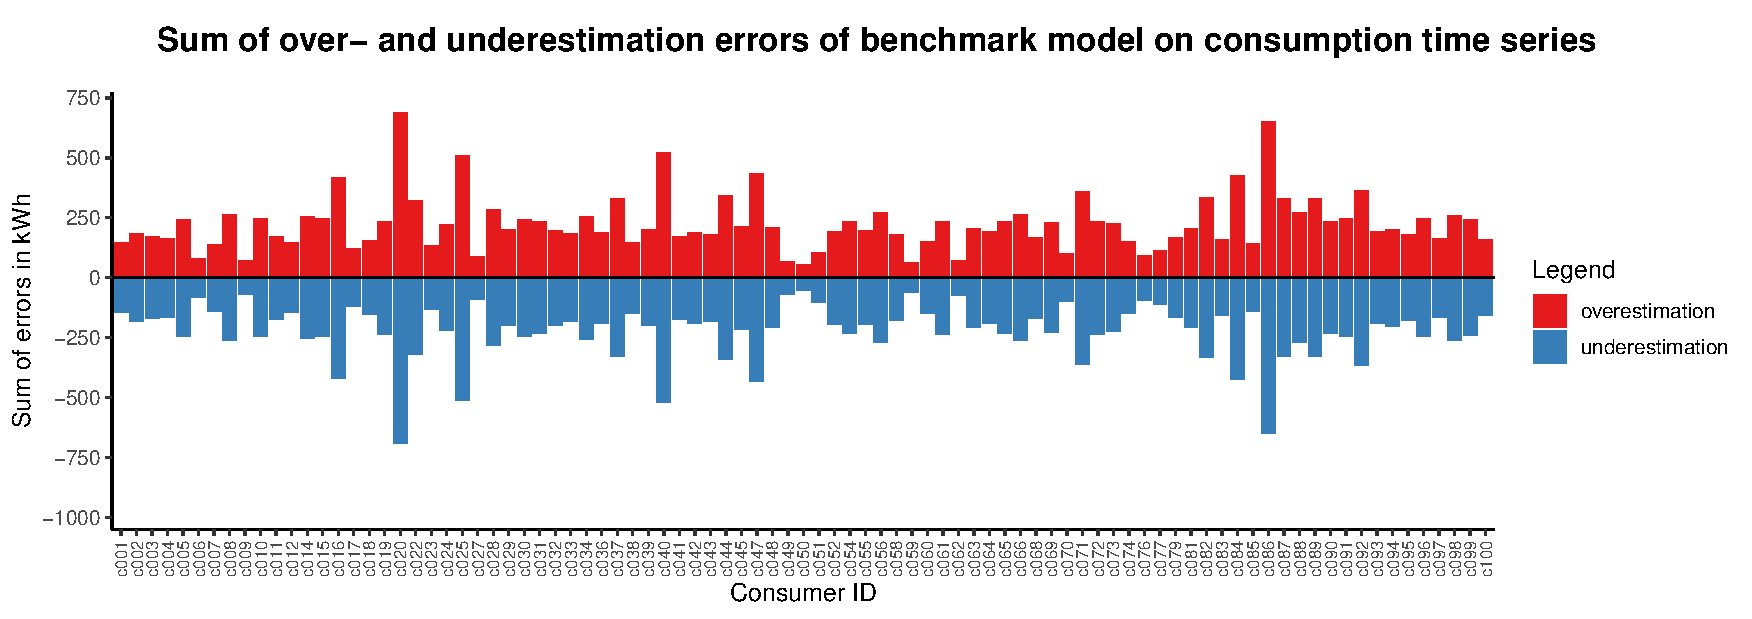
\includegraphics[width=\textwidth]{thesis/graphs/evaluation/c_barplot_naive_overunderestimation.pdf}\\\vspace{.6cm}
    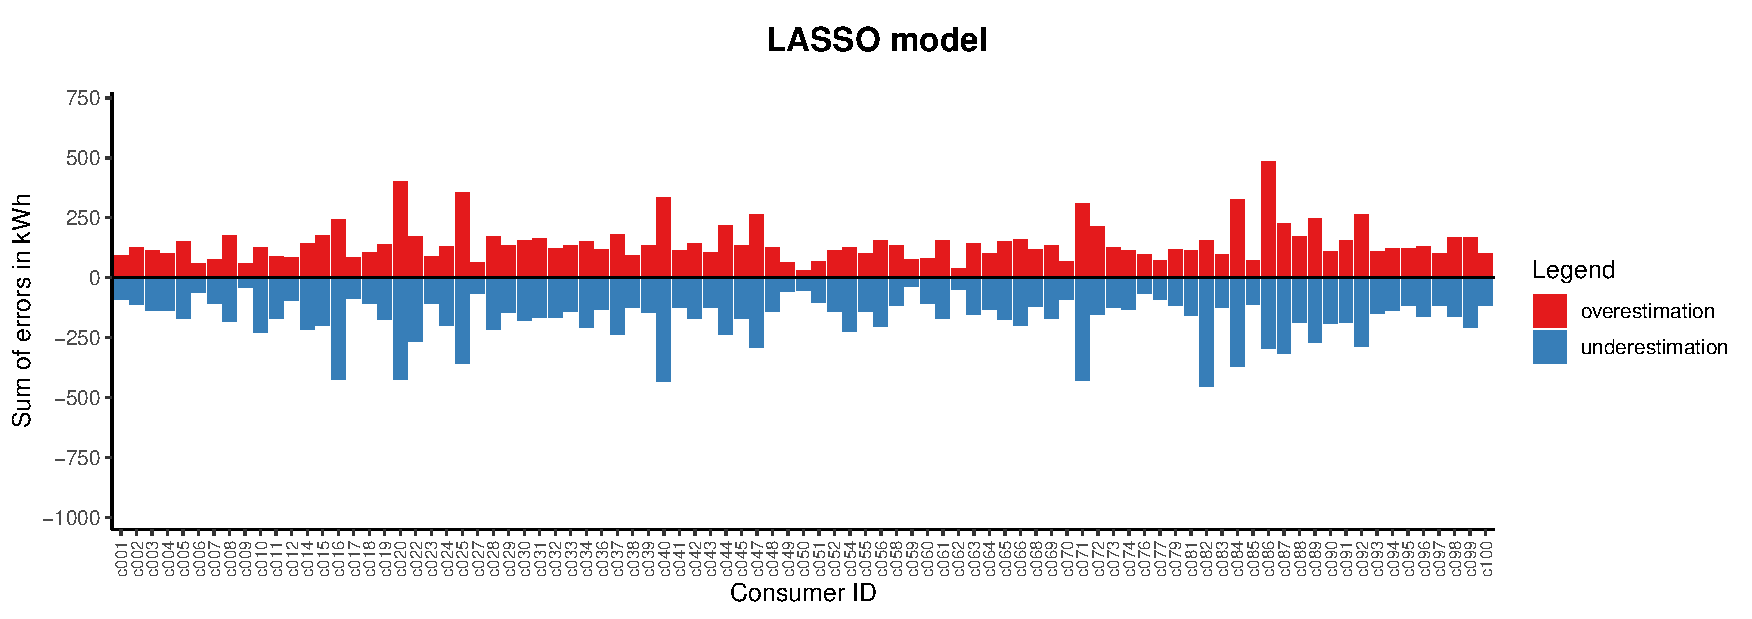
\includegraphics[width=\textwidth]{thesis/graphs/evaluation/c_barplot_LASSO_overunderestimation.pdf}\\\vspace{.6cm}
    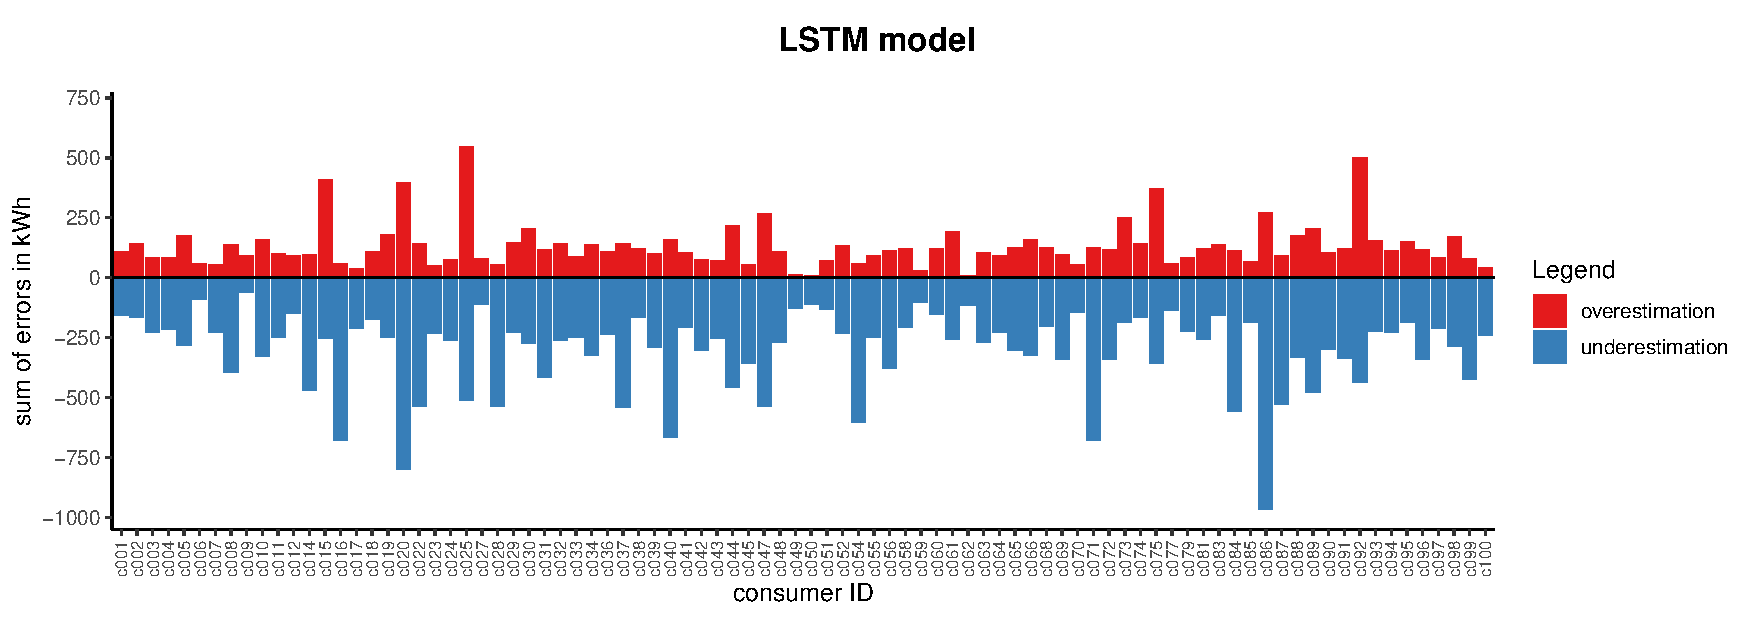
\includegraphics[width=\textwidth]{thesis/graphs/evaluation/c_barplot_LSTM_overunderestimation.pdf}
    \caption[Sum of total over- and underestimation errors per consumer data set]{Sum of total over- and underestimation errors of energy consumption per consumer data set and prediction model. \quantnet\href{https://github.com/QuantLet/BLEM/tree/master/BLEMplotPredErrors}{BLEMplotPredErrors}}
    \label{Fig:overunderestimation}
\end{figure}
%

The LSTM model on the other hand shows a much higher variability in the sums of over- and underestimation errors. By tendency, the overestimation errors of the LSTM model were smaller than those of the LASSO and benchmark models. Nevertheless, the underestimation is much more pronounced in the case of the LSTM model. Especially, some data sets stand out regarding the high sum of underestimation errors. This points towards a much higher heterogeneity in the suitability of the LSTM model to predict consumption values depending on the energy consumption pattern of the specific data set. The LASSO model on the other hand seems to be more equally well suited for all data sets and their particular consumption patterns.


The average performance of the three prediction models across all 88 data sets is shown in Table~\ref{Tab:avg_errormeasures}. As can be seen, LASSO and LSTM consistently outperformed the benchmark model according to MAE, RMSE, MAPE, and MASE. Interestingly, due to the heavy penalty NRMSE puts on comparably large prediction errors, both sophisticated prediction methods perform worse according to NRMSE, however.
%
\begingroup\catcode`"=9
\begin{table}[htbp]
{\footnotesize
    \csvreader[centered tabular=l|SSSSS,
    before reading=\sisetup{round-mode=places,round-precision=2,round-integer-to-decimal},
    filter not strcmp={\thecsvinputline}{1},
    table head=
    \hline\hline
     \multicolumn{1} {l}{\textbf{Model}} & \multicolumn{1} {c}{\textbf{MAE}} & \multicolumn{1} {c}{\textbf{RMSE}} & \multicolumn{1} {c}{\textbf{MAPE}} & \multicolumn{1} {c}{\textbf{NRMSE}} & \multicolumn{1} {c}{\textbf{MASE}}\\
    \hline,
    no head,
    separator=comma,
    respect all,
    late after line=\\,
    table foot=\hline \hline]
    {thesis/tables/avg_errorMeasures_c.csv}{}%
    {\csvcolii & \csvcoliii & \csvcoliv & \csvcolv & \csvcolvi & \csvcolvii}}%
    \caption[Mean of error measures for prediction on consumer data sets]{Mean of error measures for the prediction of energy consumption across all 88 consumer data sets. \quantnet\href{https://github.com/QuantLet/BLEM/tree/master/BLEMevaluateEnergyPreds}{BLEMevaluateEnergyPreds}}
    \label{Tab:avg_errormeasures}
\end{table}
\endgroup
%

A detailed analysis of this unexpected result reveals that it is mainly driven by an extremely bad NRMSE score for LSTM and LASSO on merely one out of the 88 data sets. As can be seen in Figure~\ref{Fig:heatmaps}, the predictions on consumer data set 027 have a particularly high NRMSE (and MAPE) compared to all other data sets. However, this pattern is not present in the absolute error measures. Further investigating the prediction errors of the forecasts on consumer 027 exposes that the high NRMSE score is driven by merely one observations: Between 24.11.2017 11:30 and 11:45 the energy consumption falls below 3 $\times$ $10^{-6}$. Due to this true value, $x_t$, which is very close to zero, the relative squared error $e_t = \left(\frac{\widehat{x}_t-x_t}{x_t}\right)^2$ is extremely high (see Appendix~\hyperlink{AppA4:Figures:erroranalysis}{A4}). This single extreme relative error pushes the NRMSE of the LSTM predictions to the staggering value of $\text{NRMSE}_{c027}=2383.46$. The same is true for MAPE, although not as extreme.
%
\begin{figure}[!ht]
 \centering
 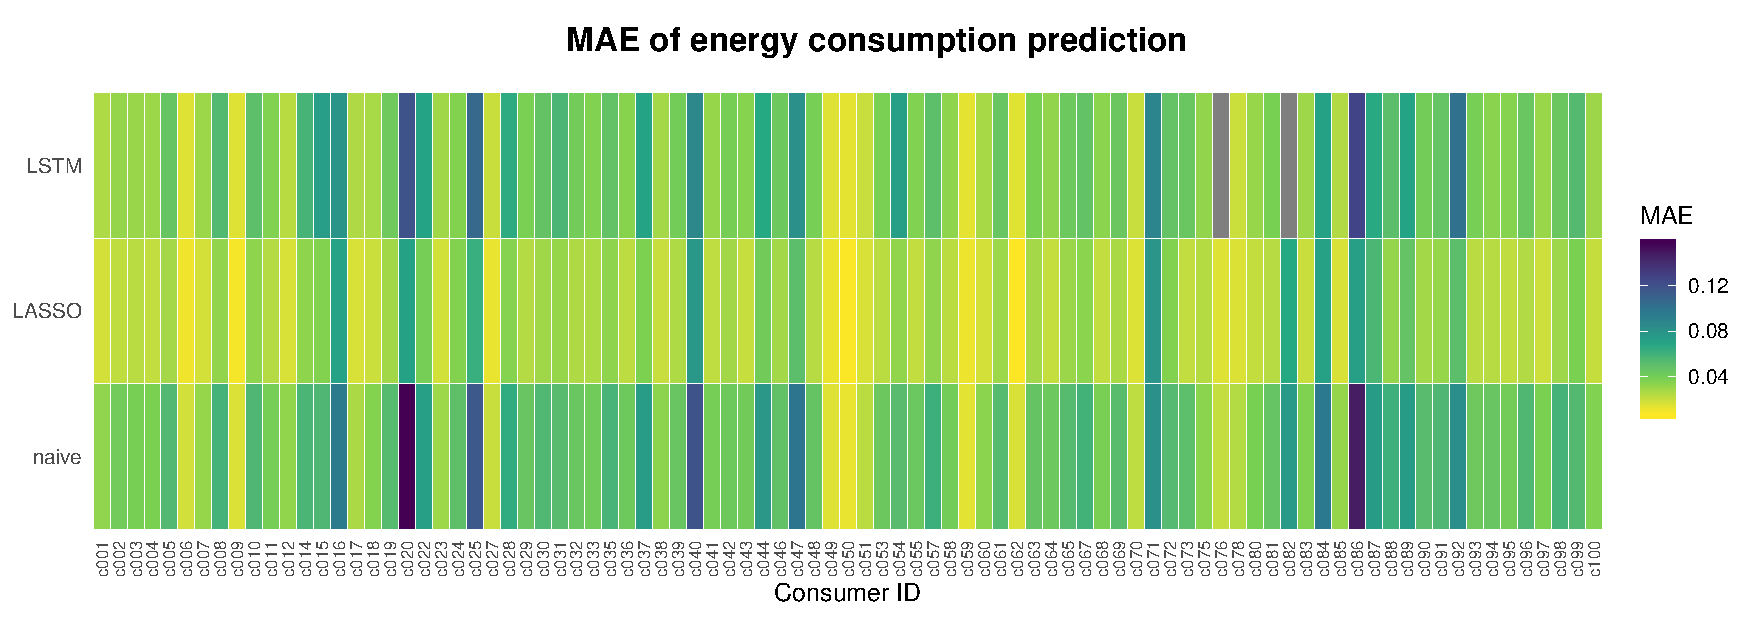
\includegraphics[width=\textwidth]{thesis/graphs/evaluation/c_heatmap_MAE.pdf}
 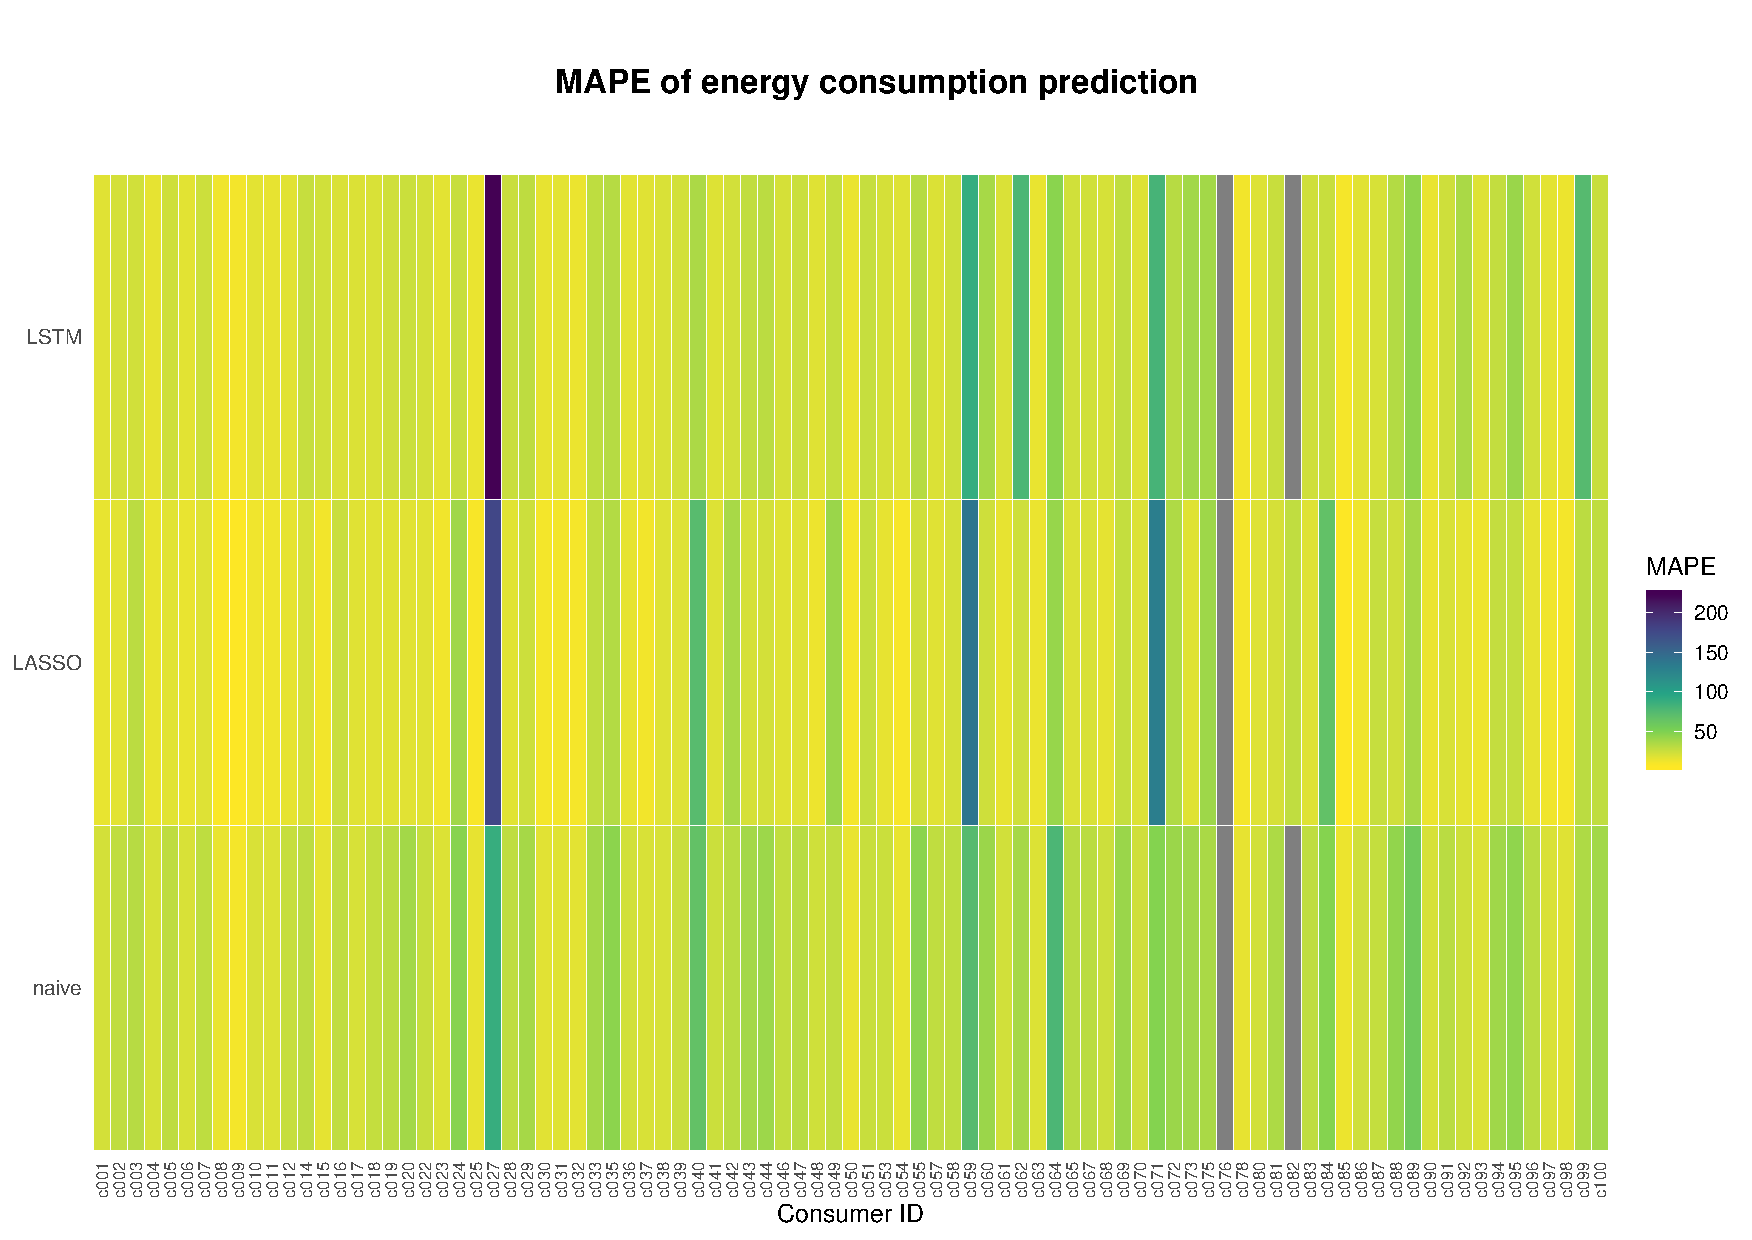
\includegraphics[width=\textwidth]{thesis/graphs/evaluation/c_heatmap_MAPE.pdf}
 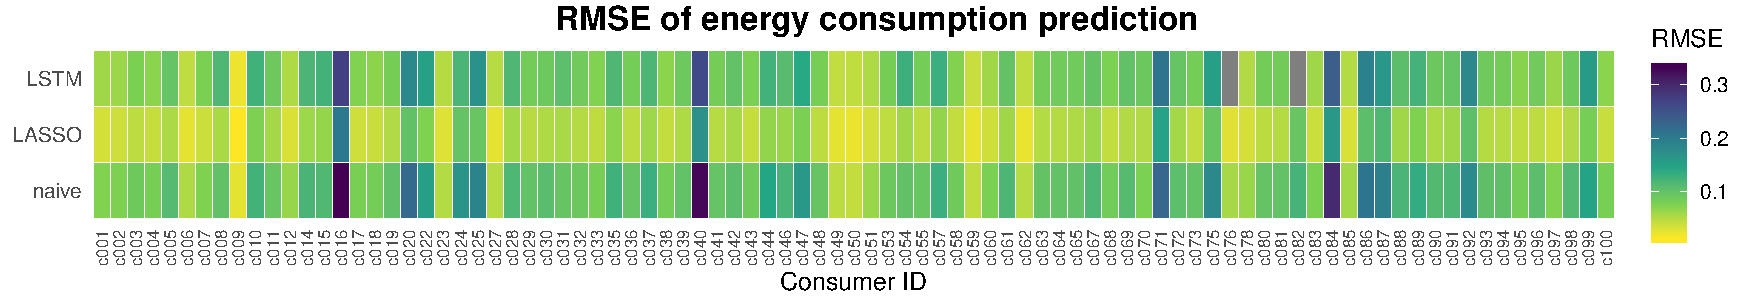
\includegraphics[width=\textwidth]{thesis/graphs/evaluation/c_heatmap_RMSE.pdf}
 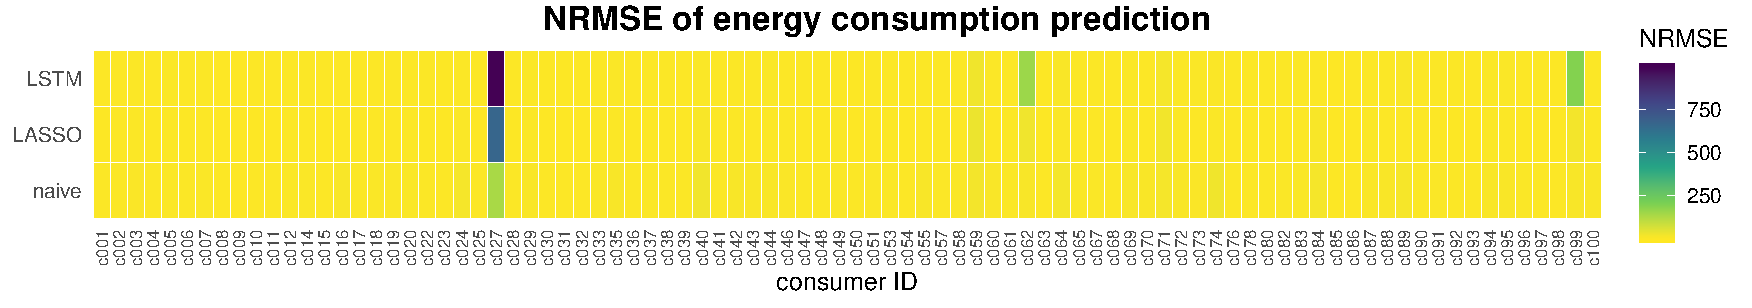
\includegraphics[width=\textwidth]{thesis/graphs/evaluation/c_heatmap_NRMSE.pdf}
 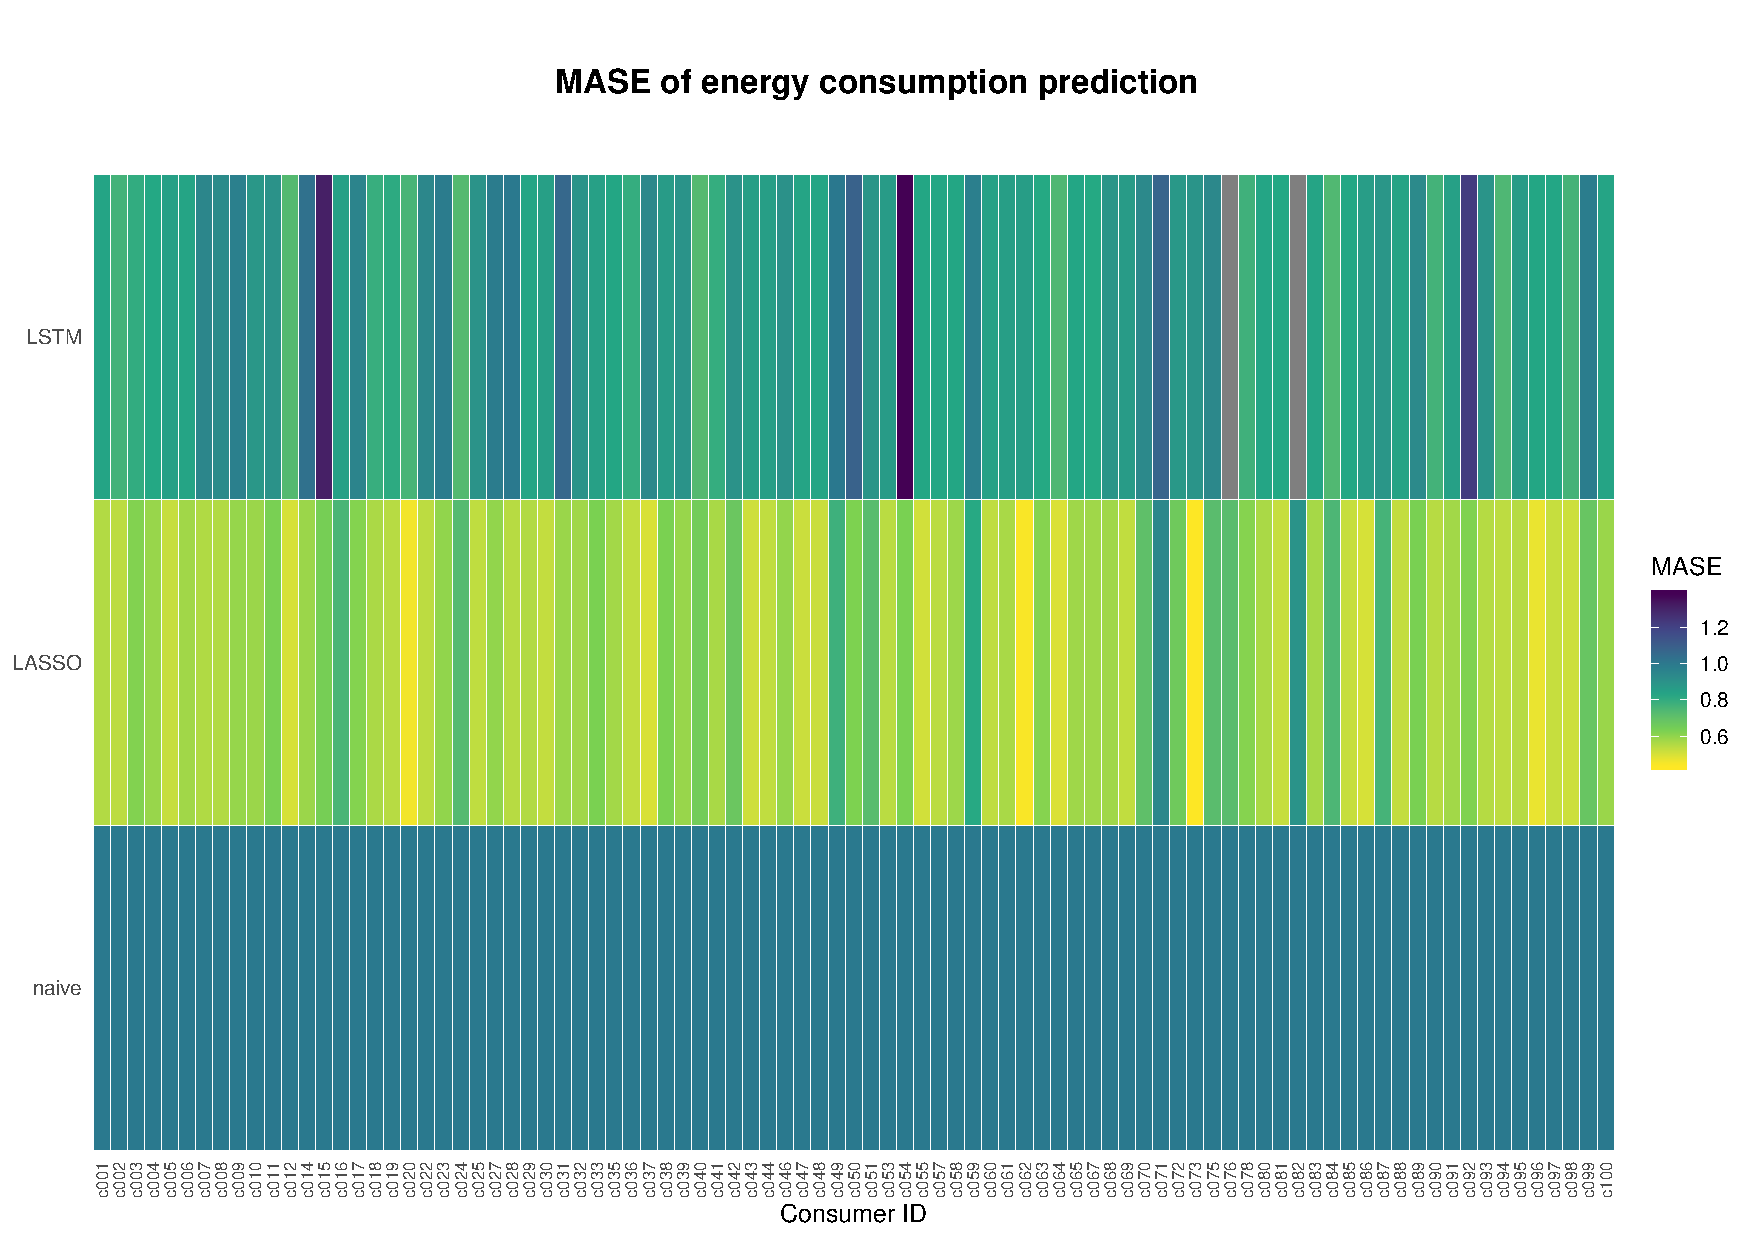
\includegraphics[width=\textwidth]{thesis/graphs/evaluation/c_heatmap_MASE.pdf}
\caption[Heatmaps of error measures for prediction of consumption values]{Heatmap of MAE, MAPE, RMSE, NRMSE, and MASE scores for the prediction of consumption values per consumer data set. \quantnet\href{https://github.com/QuantLet/BLEM/tree/master/BLEMevaluateEnergyPreds}{BLEMevaluateEnergyPreds}}
\label{Fig:heatmaps}
\end{figure}
%
 
Based on this insight, it seemed reasonable to reevaluate the average performance of the prediction methods across all consumer data sets using the median instead of the mean. Calculating the median error measures for all predictions on the consumer data sets eliminates the distortion by outliers. Thus, Table~\ref{Tab:median_errormeasures} shows the same error measures as Table~\ref{Tab:avg_errormeasures} but uses the median instead of the mean to summarize the models performance across all consumer data sets. This shows the LASSO model performed best overall with the lowest median MAE, RMSE, MAPE, NRMSE, and MASE scores. With a median MAPE across the 88 consumer datasets of 17.38~\%, it achieved an even better score in the present research than in the implementation of \citet{Li:2017}, who achieved a score of 20.06~\%.
%
\begingroup\catcode`"=9
\begin{table}[!hb]
{\footnotesize
    \csvreader[centered tabular=l|SSSSS,
    before reading=\sisetup{round-mode=places,round-precision=2,round-integer-to-decimal},
    filter not strcmp={\thecsvinputline}{1},
    table head=
    \hline\hline
     \multicolumn{1} {l}{\textbf{Model}} & \multicolumn{1} {c}{\textbf{MAE}} & \multicolumn{1} {c}{\textbf{RMSE}} & \multicolumn{1} {c}{\textbf{MAPE}} & \multicolumn{1} {c}{\textbf{NRMSE}} & \multicolumn{1} {c}{\textbf{MASE}}\\
    \hline,
    no head,
    separator=comma,
    respect all,
    late after line=\\,
    table foot=\hline \hline]
    {thesis/tables/median_errorMeasures.csv}{}%
    {\csvcolii & \csvcoliii & \csvcoliv & \csvcolv & \csvcolvi & \csvcolvii}}%
    \caption[Median of error measures for prediction on consumer data sets]{Median of error measures for the prediction of energy consumption across all 88 consumer data sets. \quantnet\href{https://github.com/QuantLet/BLEM/tree/master/BLEMevaluateEnergyPreds}{BLEMevaluateEnergyPreds}}
    \label{Tab:median_errormeasures}
\end{table}
\endgroup
%

The superior performance of the LASSO model is also clearly visible in Figure~\ref{Fig:boxplots_errormeasures}. Additionally noteworthy here are the differences in the IQR of the error measures between the prediction methods. Both, the LASSO as well as the LSTM model, have error measures with a smaller IQR across the consumer data sets than the benchmark model. Furthermore, even though the LASSO error measures consistently have the lowest median of all three prediction models, the IQR of the relative error measures MAPE and NRMSE is very similar between LASSO and LSTM.
%
\begin{figure}
    \centering
    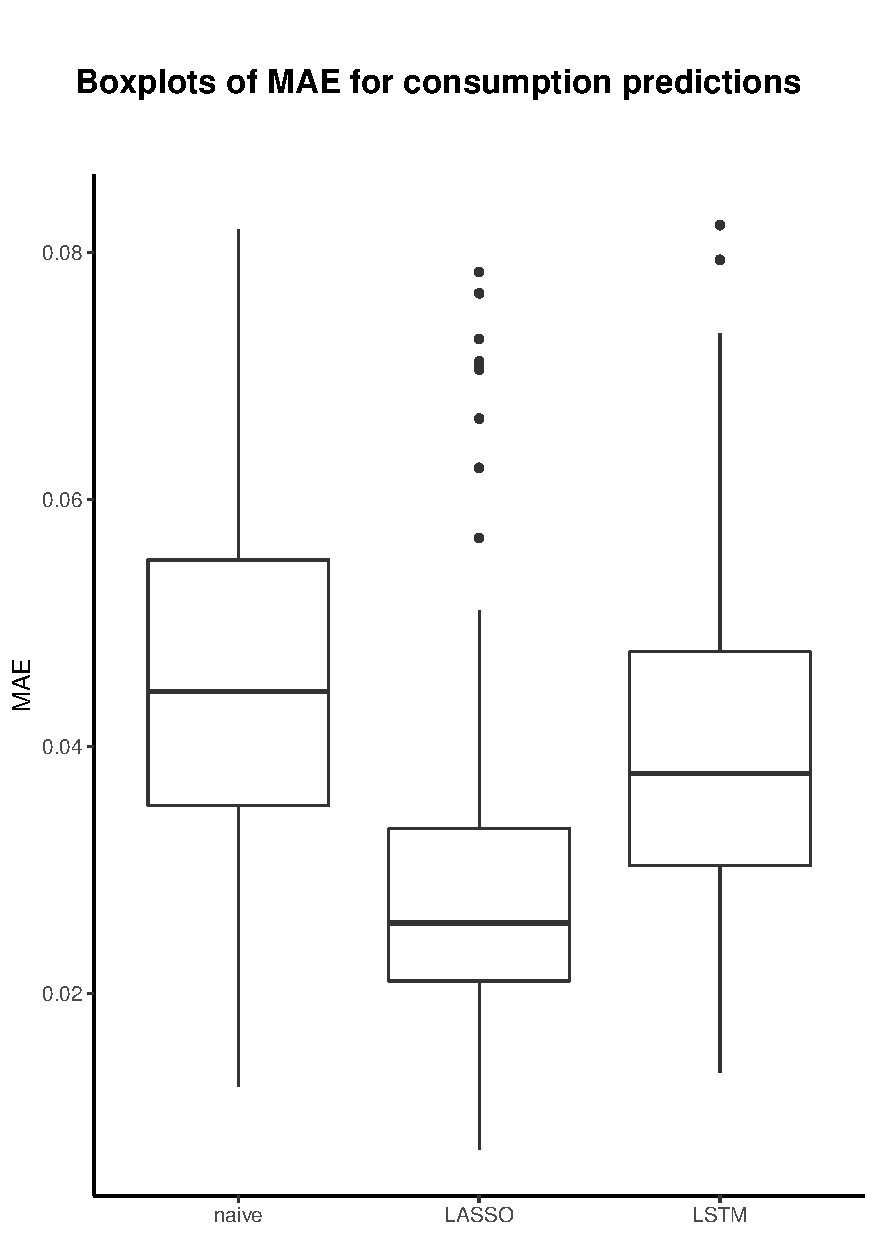
\includegraphics[width=.5\textwidth-5pt]{thesis/graphs/evaluation/c_boxplot_MAE.pdf}
    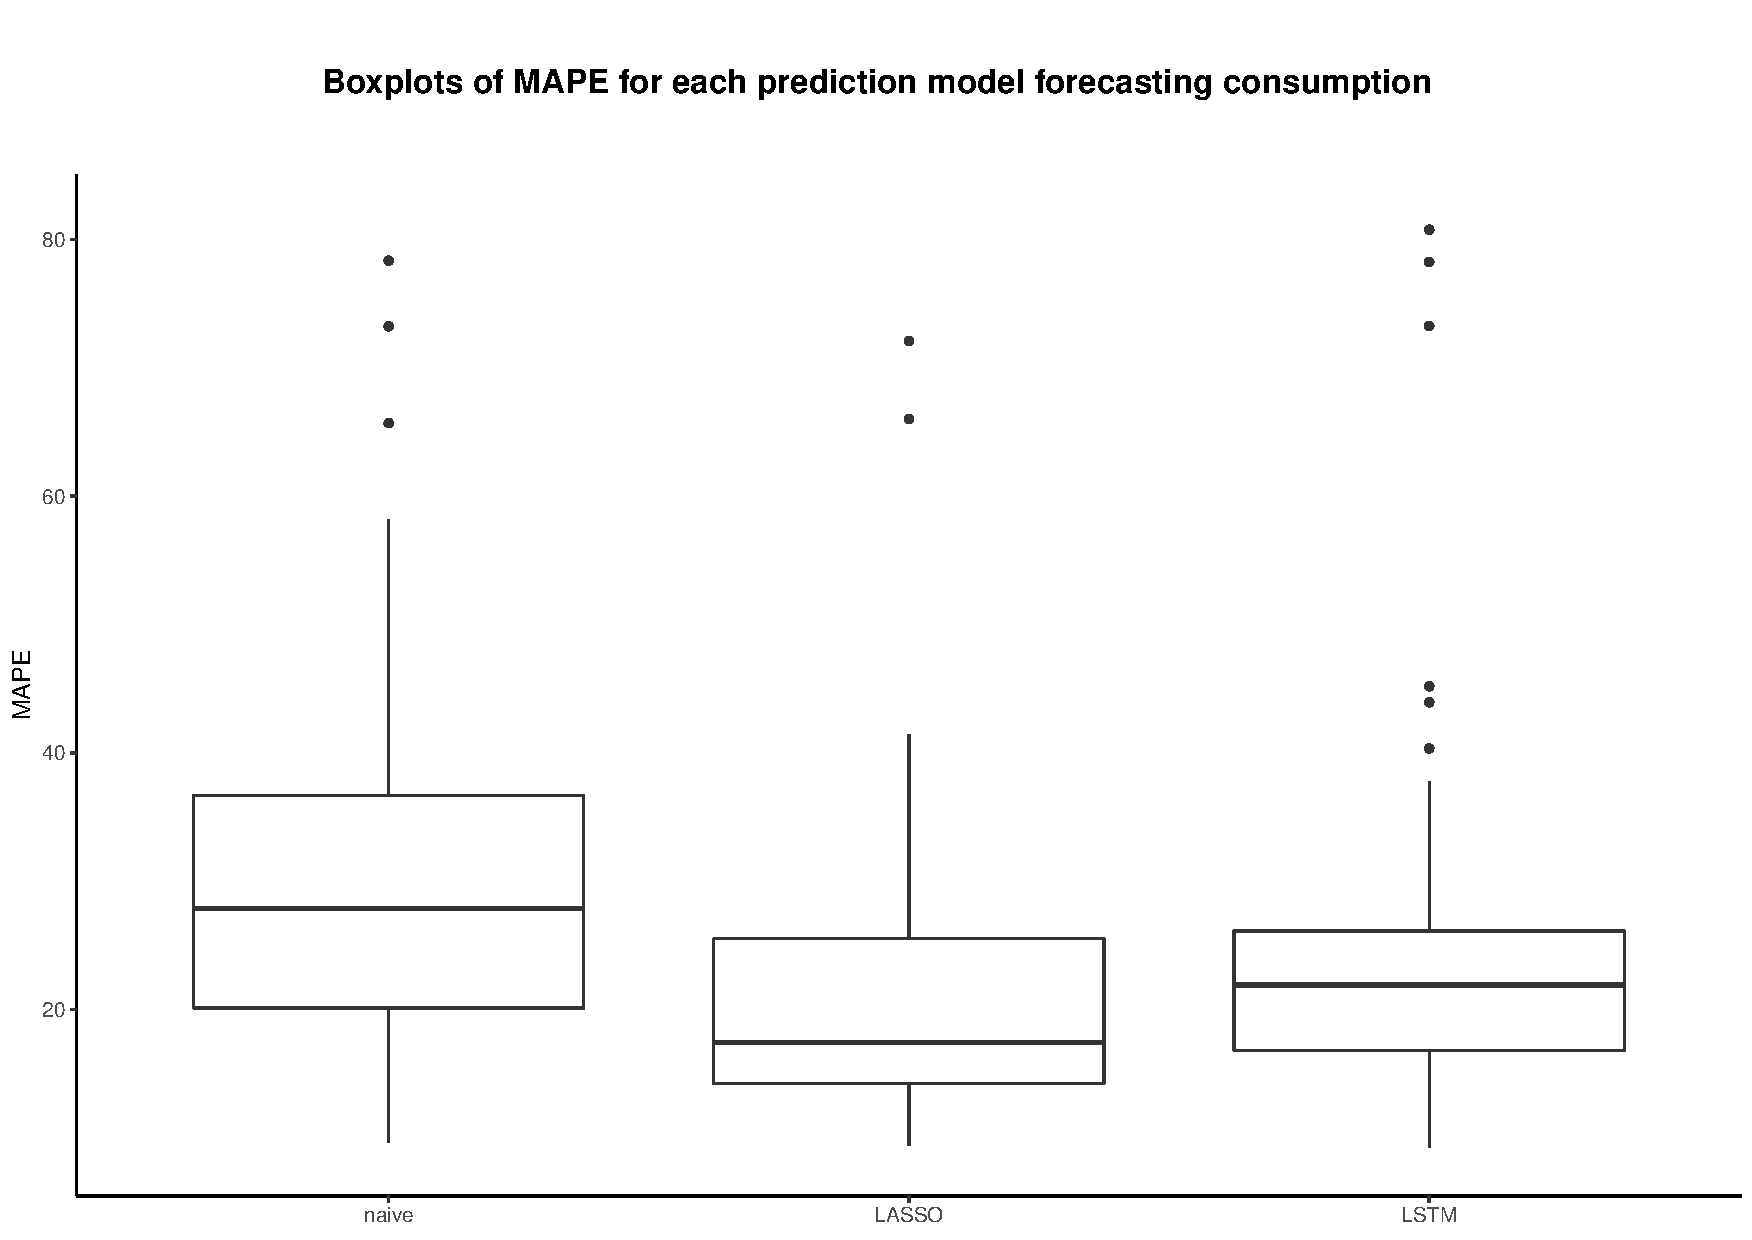
\includegraphics[width=.5\textwidth-5pt]{thesis/graphs/evaluation/c_boxplot_MAPE.pdf} \\
    
    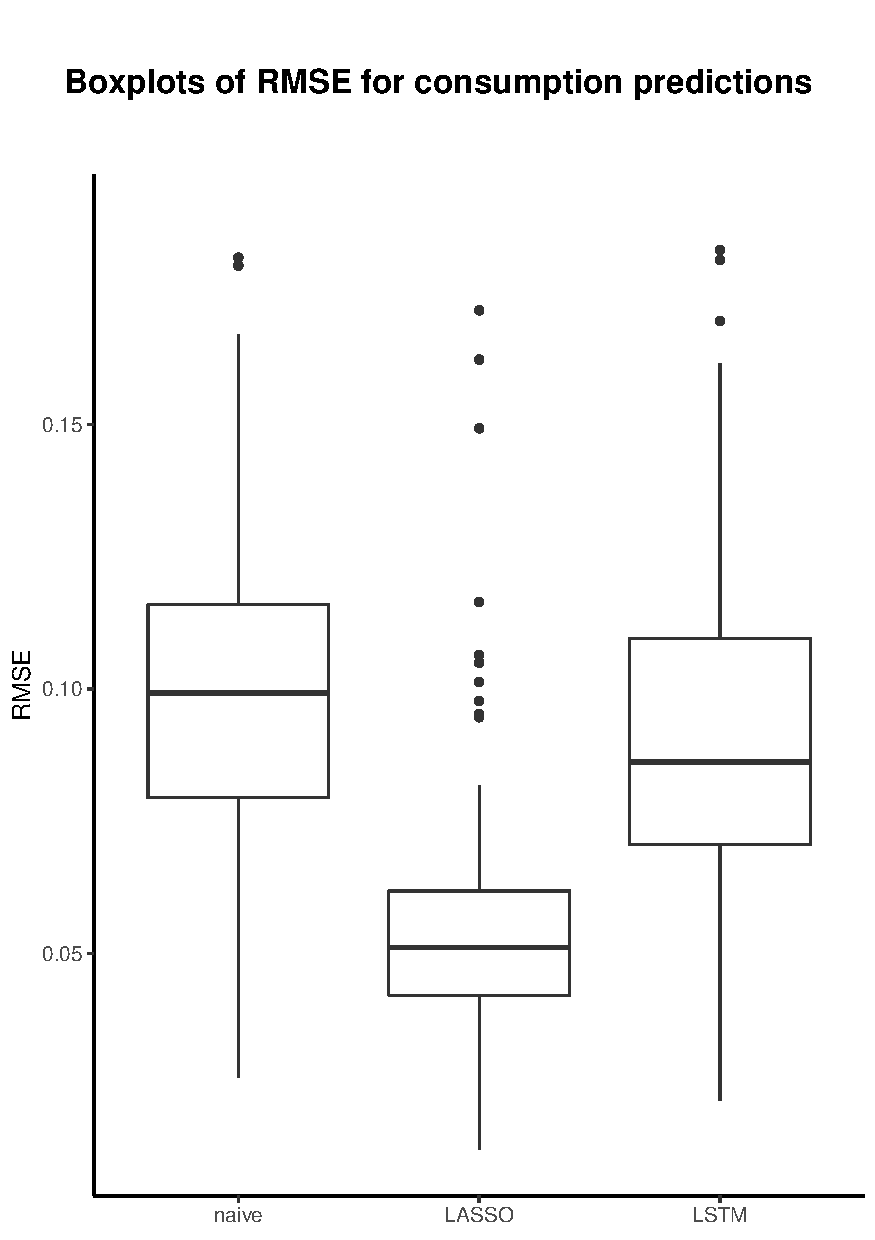
\includegraphics[width=.5\textwidth-5pt]{thesis/graphs/evaluation/c_boxplot_RMSE.pdf}
    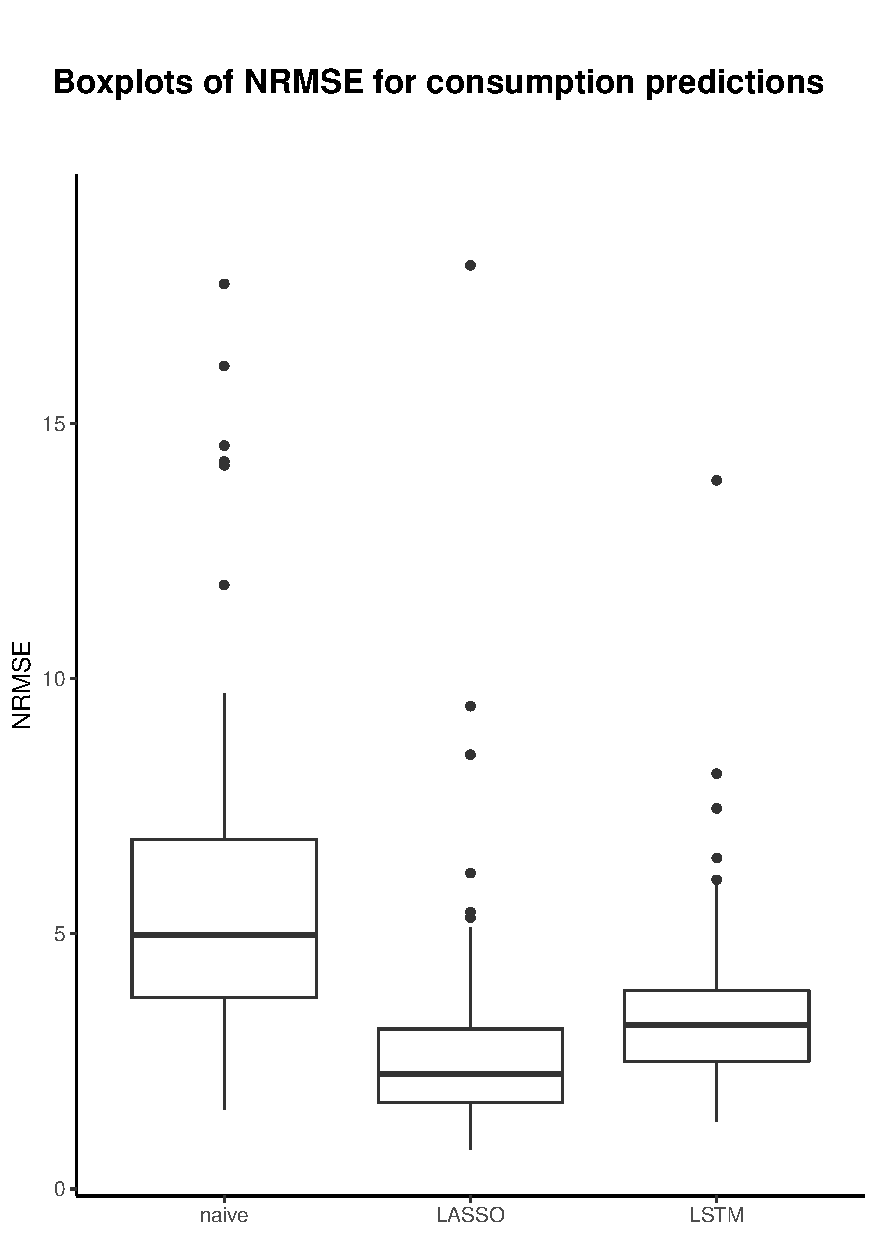
\includegraphics[width=.5\textwidth-5pt]{thesis/graphs/evaluation/c_boxplot_NRMSE.pdf} \\
    \caption[Boxplots of error measures for prediction of consumption values]{Boxplots of MAE, MAPE, RMSE, and NRMSE scores across 88 consumer data sets for the three different prediction models (the upper 3~\%-quantile of the error measures is cut off for better readability). \quantnet\href{https://github.com/QuantLet/BLEM/tree/master/BLEMevaluateEnergyPreds}{BLEMevaluateEnergyPreds}}
    \label{Fig:boxplots_errormeasures}
\end{figure}
%

\newpage
Interestingly, there are some consumer data sets which exhibit apparently much harder to predict consumption patterns than the other data sets. This is exemplified by the outliers of the MAPE and NRMSE boxplots, and also, by the heatmaps displayed in Figure~\ref{Fig:heatmaps}. Unfortunately, the heatmaps of the relative error measures MAPE and NRMSE are dominated by the very high values for consumer 027. An alternative way to calculate those error measures according to \citet{Hyndman:2006} to avoid very skewed NRMSE or MAPE distribution in the presence of values close to zero is to use the median instead of the mean error. Thus, the mean absolute percentage error becomes the median absolute percentage error (MdAPE) and the normalized root mean squared error becomes the normalized root median squared error (NRMdSE). Taking consumer 027 as an example, the difference becomes clear: The normalized root mean squared error is $\text{NRMSE}_{c027}=2383.46$, while the normalized root \emph{median} squared error is only $\text{NRMdSE}_{c027}=33.43$ (which is still comparatively high). The same holds true for MAPE and MdAPE\footnote{The average MdAPE and NRMdSE across all consumer data sets in comparison to MAPE and NRMSE are presented in Appendix~\hyperlink{AppB2:Tables:avg_errM_wMedian}{B2}.}. Accordingly, the heatmaps for MdAPE and NRMdSE are shown in Figure~\ref{Fig:heatmaps_median}. They confirm that there is a wide variation in the performance of the same prediction methods on the same kind of data but from different households. Therefore one can conclude, that apparently, there is no ``one-size-fits-all'' approach for households' very short-term energy consumption forecasting.

%
\begin{figure}[ht]
 \centering
 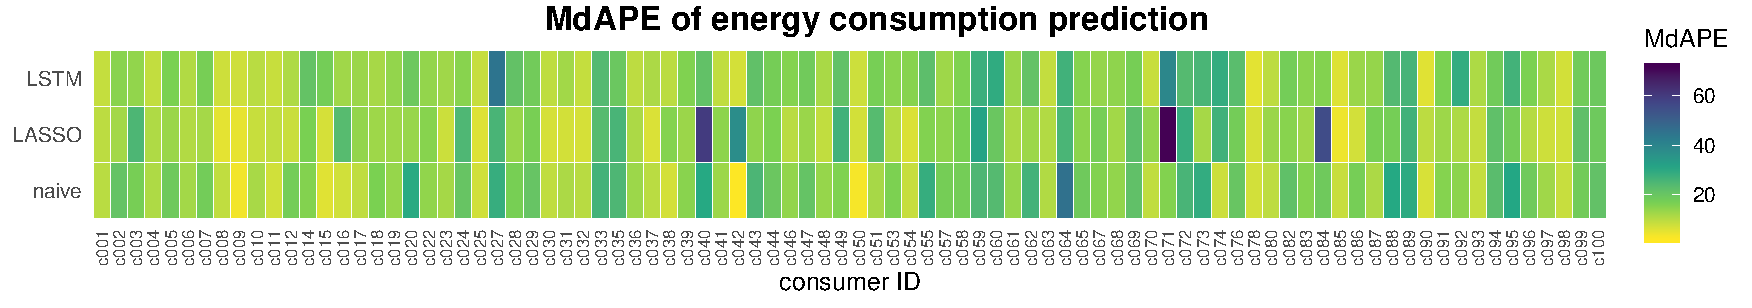
\includegraphics[width=\textwidth]{thesis/graphs/evaluation/c_heatmap_MdAPE.pdf}
 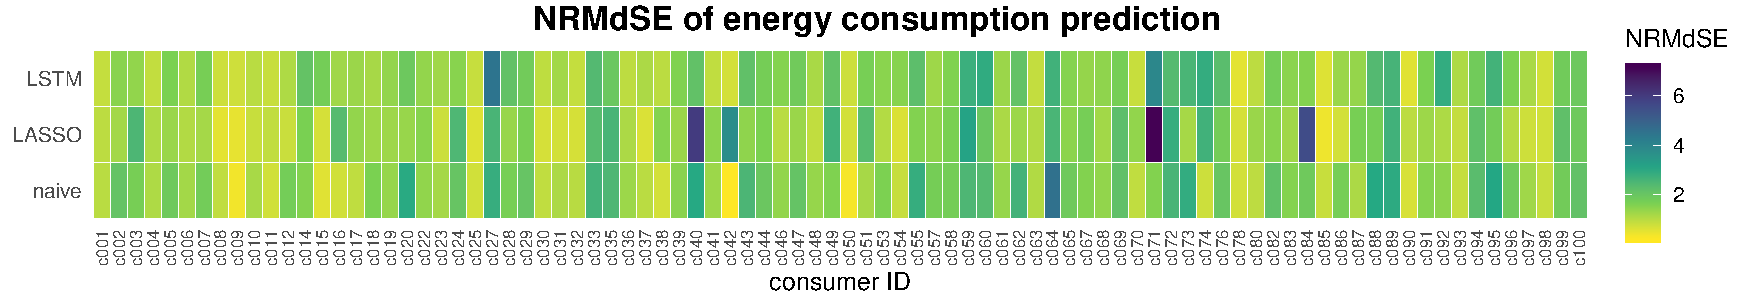
\includegraphics[width=\textwidth]{thesis/graphs/evaluation/c_heatmap_NRMdSE.pdf}
\caption[Heatmaps of MdAPE and NRMdSE for consumption values]{Heatmap of MdAPE and NRMdSE scores for the prediction of consumption values per consumer data set. \quantnet\href{https://github.com/QuantLet/BLEM/tree/master/BLEMevaluateEnergyPreds}{BLEMevaluateEnergyPreds}}
\label{Fig:heatmaps_median}
\end{figure}
%

Nevertheless, it is obvious that the LASSO model performed best overall. Hence, the predictions on the last quarter of the data produced by the fitted LASSO model for each consumer data set will be used for the evaluation of the following market simulation.



%%%%%%%%%%%
\subsubsection{Production data}

Also for the production data, the performance of the prediction models was tested on a quarter of the production time series. That is, the prediction models were fitted on the production values from 01.01.2017~00:00 to 30.09.2017~00:00 which is equivalent to 131,040 data points per data set. For all 12 prosumer data sets, the models were fitted separately resulting in as many distinct LASSO and LSTM prediction models. The fitted models were then used to make energy production predictions in 15-minutes intervals for each household individually on the data from 01.10.2017~00:00 to 01.01.2018~00:00. This equates to 8,836 predicted values per data set per prediction method.

Figure~\ref{Fig:glimpse_predprod} exemplary shows the true and predicted production values of prosumer 024 on December 23, 2017. The na\"ive benchmark model just follows the true production shifted by one time step (i.e., 15 minutes). As in the consumption predictions, this fits the true values generally good, as long as there are no sudden spikes in the household's energy production. Spikes or sudden drops in energy production -- as in this example one occurred in the 15 minutes before 06:00 a.m.~-- necessarily lead to a prediction with high error of the na\"ive predictor. In such situations, the LASSO model seems more accurate. Even though, it underestimates the spike in energy production in this example, it does not lag behind as much as the na\"ive predictor and, generally, has the ability to anticipate movements. The LSTM-based predictions, on the contrary, fit even worse than the na\"ive predictor in this example. They almost do not at all follow small movements in the energy production time series and lag behind the true values similarly to the na\"ive predictor. Also, the LSTM model constantly overestimates in periods of zero production and does not follow the upward spike in energy production present in this exemplary snippet of the data.
%
\begin{figure}[htbp]
    \centering
    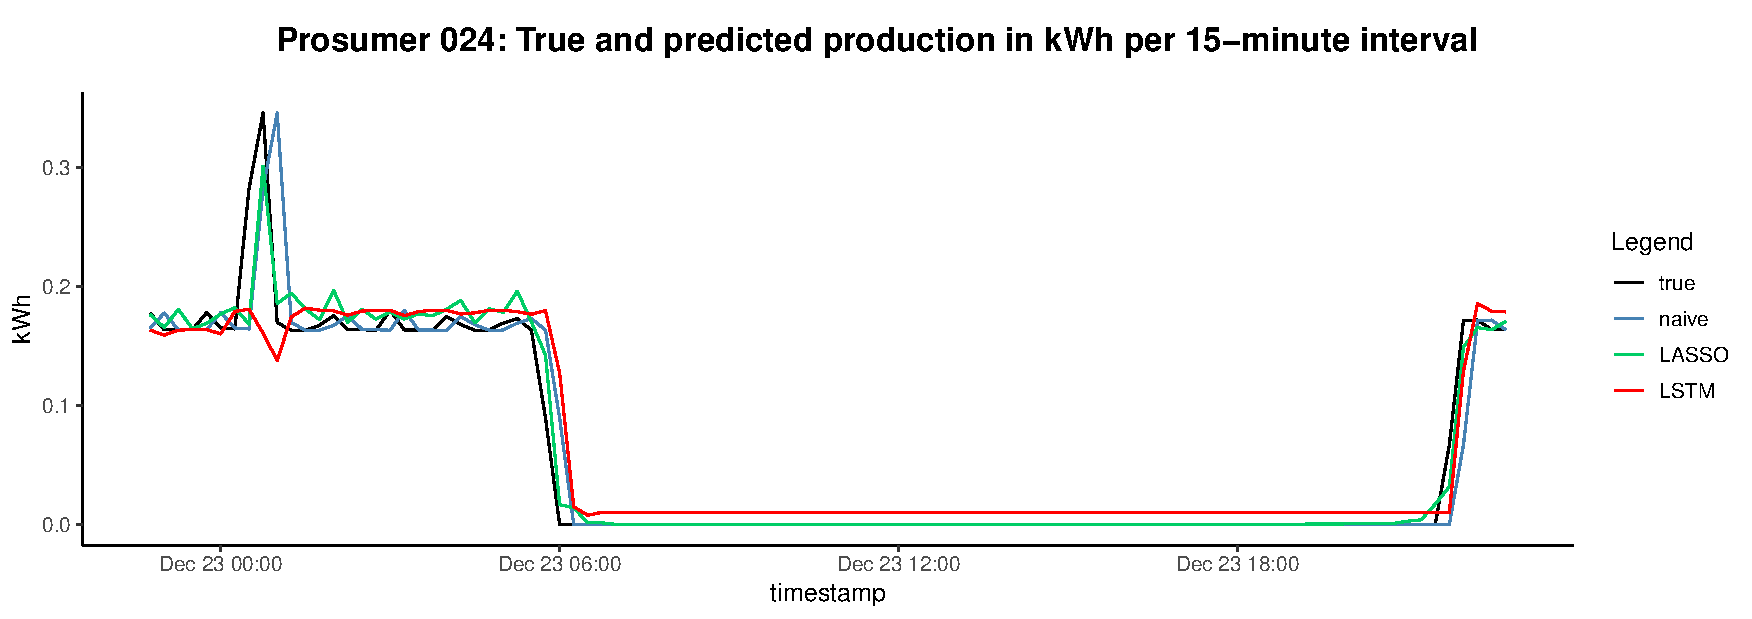
\includegraphics[width=\textwidth]{thesis/graphs/evaluation/p024_pred_prod.pdf}
    \caption[Exemplary 24 hours of true and predicted production values]{Exemplary 24 hours of true and predicted production values of prosumer 024. \quantnet\href{https://github.com/QuantLet/BLEM/tree/master/BLEMplotEnergyPreds}{BLEMplotEnergyPreds}}
    \label{Fig:glimpse_predprod}
\end{figure}
%

Analyzing the over- and underestimation errors of each prediction method on each producer data set shows the extreme tendency of the LSTM model to underestimate the production values (see Figure~\ref{Fig:overunderestimation_p}).
%
\begin{figure}[!h]
    \centering
    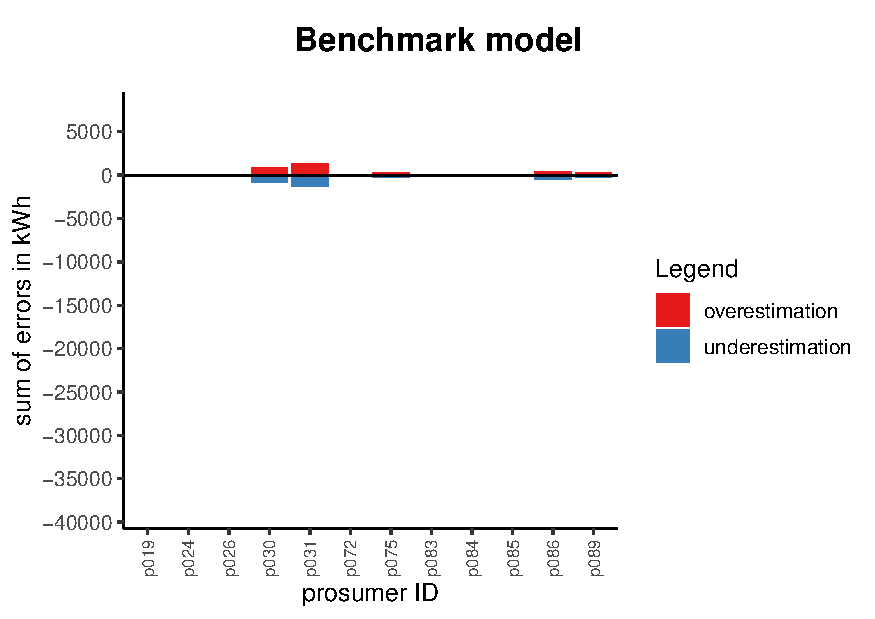
\includegraphics[width=.5\textwidth]{thesis/graphs/evaluation/p_barplot_naive_overunderestimation.pdf}\\\vspace{.6cm}
    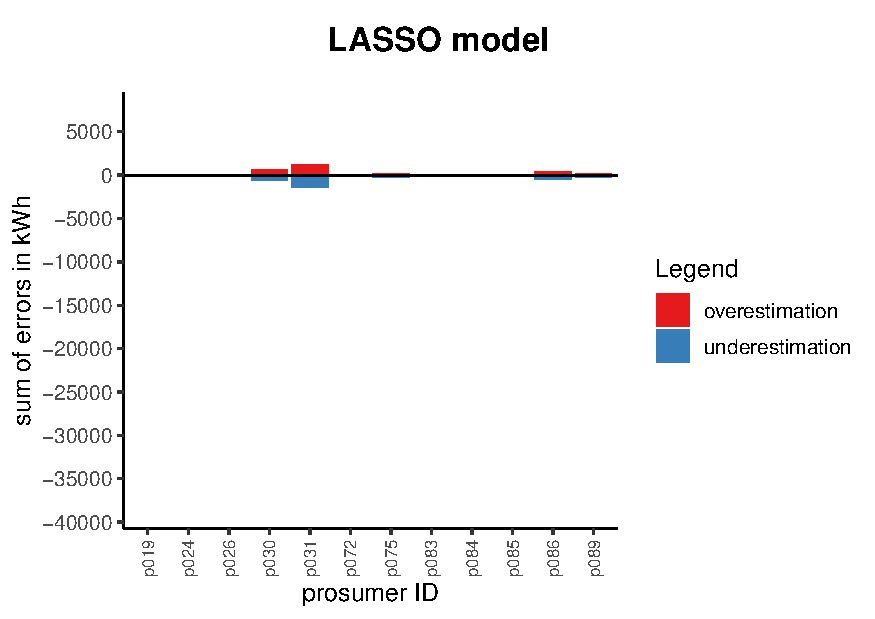
\includegraphics[width=.5\textwidth]{thesis/graphs/evaluation/p_barplot_LASSO_overunderestimation.pdf}\\\vspace{.6cm}
    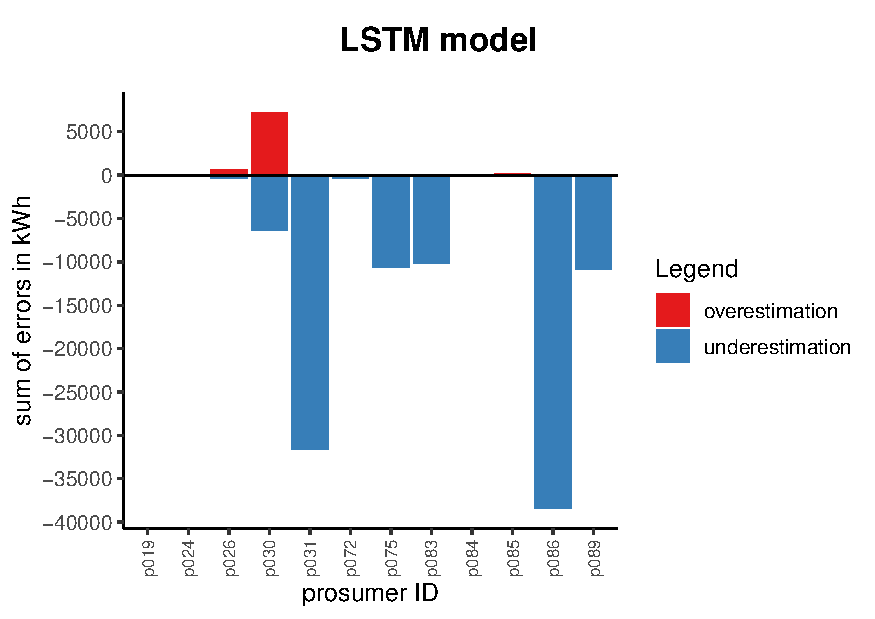
\includegraphics[width=.5\textwidth]{thesis/graphs/evaluation/p_barplot_LSTM_overunderestimation.pdf}
    \caption[Sum of total over- and underestimation errors per prosumer data set]{Sum of total over- and underestimation errors of energy production per prosumer data set and prediction model. \quantnet\href{https://github.com/QuantLet/BLEM/tree/master/BLEMplotPredErrors}{BLEMplotPredErrors}}
    \label{Fig:overunderestimation_p}
\end{figure}
%

The LSTM's sum of underestimation errors is substantially larger for six out of twelve prosumer data sets and the sum of overestimation is substantially larger for one data set compared to the LASSO and benchmark model. This already indicates a much worse performance of LSTM than LASSO or the na\"ive predictor on the production data.

The first impression is confirmed by the average of the error measures across the 12 prosumer data sets shown in Table~\ref{Tab:avg_errormeasures_p}. The LSTM model on average performs much worse than the LASSO and the benchmark model according to MAE, RMSE, and MASE. Computing the median across the 12 prosumer data sets gives the same qualitative results, although the performance differences are not as extreme (see Appendix~\hyperlink{AppB3:Tables:medain_errM_prod}{B3}). MAPE and NRMSE cannot be computed as all production time series contain zero values\footnote{As can be seen in Equation~\ref{Eq:MAPE} and Equation~\ref{Eq:NRMSE}, MAPE and NRMSE are not defined if the true value $x_t$ equals zero which is why they cannot be computed for the predictions on production data.}.
%
\begingroup\catcode`"=9
\begin{table}[ht]
{\footnotesize
    \csvreader[centered tabular=l|SSS,
    before reading=\sisetup{round-mode=places,round-precision=2,round-integer-to-decimal},
    filter not strcmp={\thecsvinputline}{1},
    table head=
    \hline\hline
     \multicolumn{1} {l}{\textbf{Model}} & \multicolumn{1} {c}{\textbf{MAE}} & \multicolumn{1} {c}{\textbf{RMSE}} & \multicolumn{1} {c}{\textbf{MASE}}\\
    \hline,
    no head,
    separator=comma,
    respect all,
    late after line=\\,
    table foot=\hline \hline]
    {thesis/tables/avg_errorMeasures_p.csv}{}%
    {\csvcolii & \csvcoliii & \csvcoliv & \csvcolv}}%
    \caption[Mean of error measures for prediction on prosumer data sets]{Mean of error measures for the prediction of energy production across all 12 prosumer data sets. \quantnet\href{https://github.com/QuantLet/BLEM/tree/master/BLEMevaluateEnergyPreds}{BLEMevaluateEnergyPreds}}
    \label{Tab:avg_errormeasures_p}
\end{table}
\endgroup
%

Overall, it becomes clear that the chosen prediction methods do not forecast energy production of the given prosumer data sets very well. According to the average MASE, the LASSO model is just as good as the benchmark, while the LSTM model performs much worse. A detailed comparison of the error measures for each prosumer data set as heatmap is shown in Appendix~\hyperlink{AppA5:Figures:heatmaps_p}{A5}. Due to the unsatisfying performance of the prediction methods on the production data, the predicted production values were not used in the market simulation. This means, the effect of prediction errors on market outcomes was only evaluated using the predictions of consumption values. The production values, on the contrary, were always assumed to be known in advance.

% In the case of the LSTM model, this may be due to the hyperparameter tuning being performed on a consumer data set. Moreover, the production data contains much more jumps and discontinuities than the consumption data which aggravates the prediction task.


%%%%%%%%%%%%%%%%%%%%%%%%%%%%%
%%%   Market simulation   %%%
%%%%%%%%%%%%%%%%%%%%%%%%%%%%%

\subsection{Evaluation of the market simulation}\label{Sec:Results;Subsec:Simulation}

The market simulation used the market mechanism implemented by \citet{Mengelkamp:2018a} in a smart contract to assess the impact of prediction errors on market outcomes. The data sets available for this comprised 88 consumers and 12 prosumers. To evaluate different supply scenarios, the market simulation was conducted three times with a varying number of prosumers included. The three scenarios consisted of a market simulation with balanced energy supply and demand, a simulation with severe oversupply and a simulation with severe undersupply. To avoid extreme and unusual market outcomes over the time period of the simulation, two prosumers (031 and 086) with high production levels, but long periods of no energy production in the simulation period were not included as energy suppliers in the market (see Appendix~\hyperlink{AppA7:Figures:producer_all}{A7}). The remaining prosumers were in- or excluded according to the desired supply scenario. That is, the undersupply scenario comprised prosumer 019, 024, 026, 072, 075, and 089, the balanced supply scenario additionally included prosumer 030, and the oversupply scenario additionally included prosumer 083 and 084.

%%%%%%%%%%%
\subsubsection{Market outcomes in different supply scenarios}

The difference between supply and demand for each trading period, the equilibrium price of each double auction, and the weighted average price -- termed LEM price -- is shown in Figure~\ref{Fig:marketoutcomes_true_balanced}. The LEM price is computed in each trading period as the average of the auctions equilibrium price and the energy utilities energy price (28.69 $\frac{\text{EURct}}{\text{kWh}}$) weighted by the amount of kWh traded for the respective price. Therefore, in any trading period with higher demand than supply, the LEM price will be greater or equal to the equilibrium price as the equilibrium price's upper limit is the utilities energy price of 28.69 $\frac{\text{EURct}}{\text{kWh}}$. All graphs depicting the market outcomes shown in this section are results of the market simulation with true consumption values. The equivalent graphs for the market simulation with energy consumption values predicted by a LASSO model are shown in Appendix~\hyperlink{AppA7:Figures:marketsimulation_pred}{A7}. As the graphs contain only over-/undersupply and market prices, they are not substantially different when simulating the market mechanism with predicted consumption values (as the prediction accuracy is reasonably good). Though, this is not the case for the energy cost that consumers have to bear, as is shown in the next section.

As can be seen, the equilibrium price shown in the middle panel of Figure~\ref{Fig:marketoutcomes_true_balanced} moves roughly synchronous to the over-/undersupply shown in the upper panel. As there is by tendency more undersupply in the balanced scenario (the red line in the upper panel indicates perfectly balanced supply and demand), the equilibrium price is in most trading periods close to its upper limit and the LEM price is almost always above the equilibrium price\footnote{Due to the fact that four of the relevant prosumer data sets are from producers with large capacities ($>$10 kWh per 15-minutes interval) which dominated the remaining prosumers' production capacity substantially (see also Appendix~\hyperlink{AppA7:Figures:producer_all}{A7}), it was not possible to construct a prosumer sample that better matched the market demand in the balanced supply scenario.}.
%
\begin{figure}[htp]
    \centering
    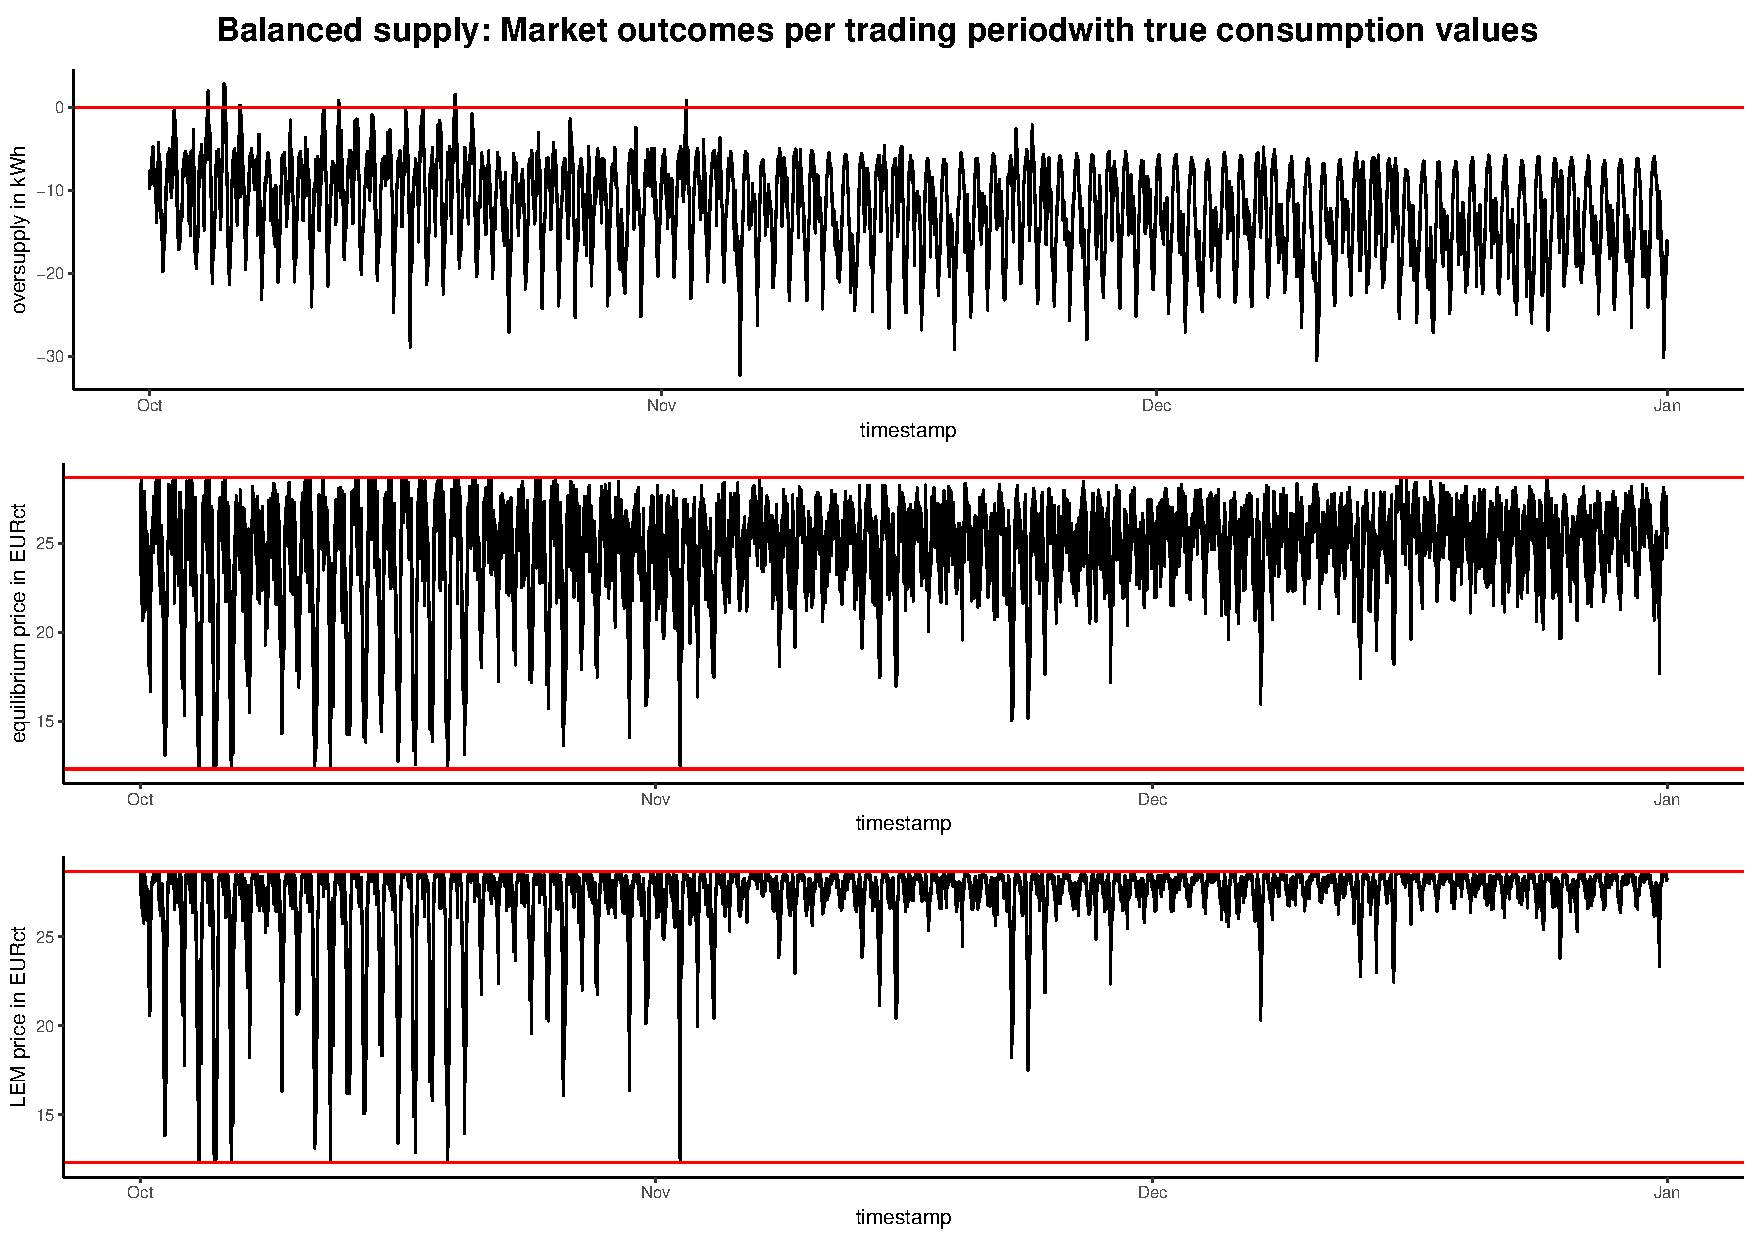
\includegraphics[width=\textwidth-1.1cm]{thesis/graphs/marketsimulation/marketoutcome_true_balanced.pdf}
    \caption[Market outcomes simulated with balanced supply and true values]{Market outcomes per trading period simulated with true values and a balanced supply scenario. \quantnet\href{https://github.com/QuantLet/BLEM/tree/master/BLEMmarketSimulation}{BLEMmarketSimulation}}
    \label{Fig:marketoutcomes_true_balanced}
\end{figure}
%

This is very much contrasted by the oversupply scenario shown in Figure~\ref{Fig:marketoutcomes_true_over}. Here, the prosumers' energy supply surpasses the consumers' energy demand in the majority of trading periods. Accordingly, the equilibrium price in each auction is close to the lower limit of the energy utility's feed-in tariff of 12.31 $\frac{\text{EURct}}{\text{kWh}}$. Still, trading periods with undersupply lead to visible spikes in the equilibrium price which are, as expected, even more pronounced in the LEM price. In all other periods, the equilibrium price equals the LEM price as all demand is served by the prosumers and there is no energy purchased from the grid.
%
\begin{figure}[htp]
    \centering
    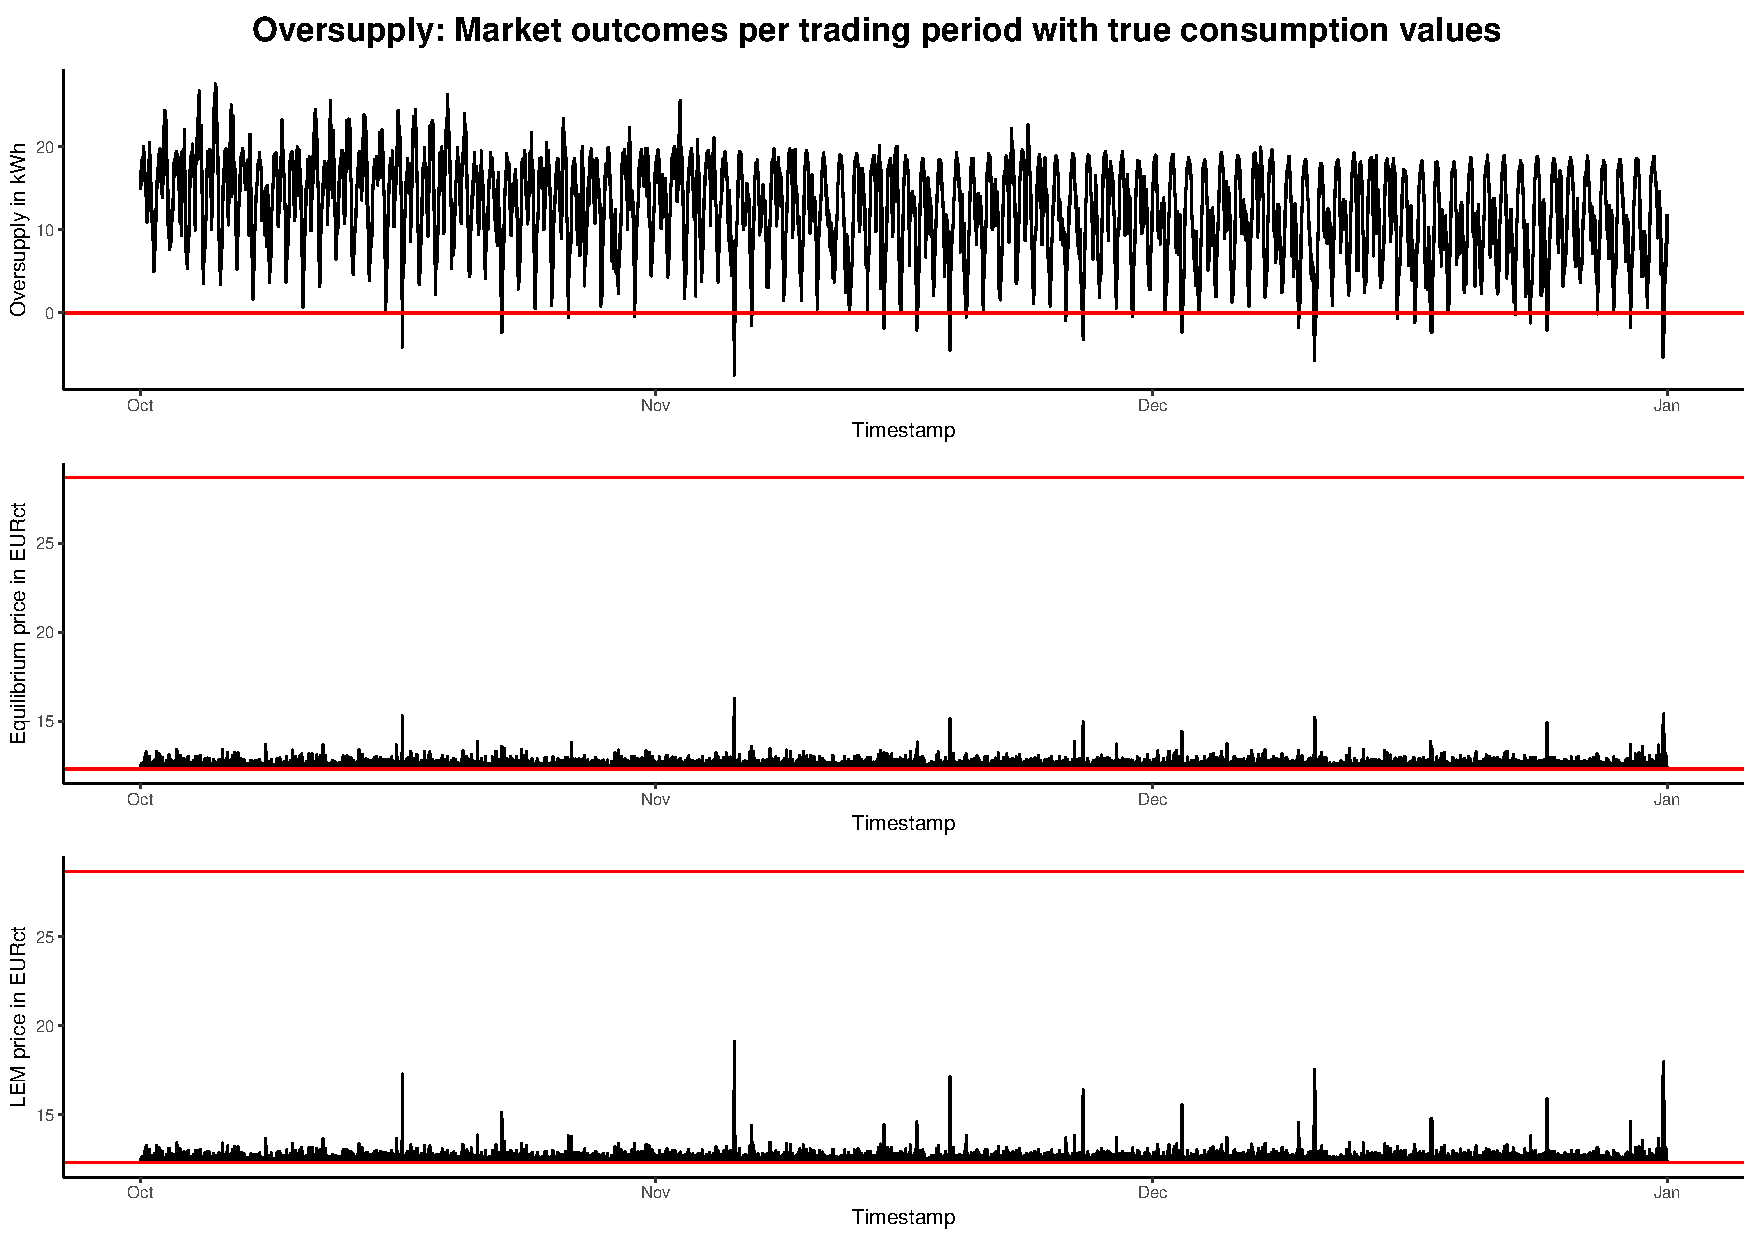
\includegraphics[width=\textwidth-1.1cm]{thesis/graphs/marketsimulation/marketoutcome_true_oversupply.pdf}
    \caption[Market outcomes simulated with oversupply and true values]{Market outcomes per trading period simulated with true values and an oversupply scenario. \quantnet\href{https://github.com/QuantLet/BLEM/tree/master/BLEMmarketSimulation}{BLEMmarketSimulation}}
    \label{Fig:marketoutcomes_true_over}
\end{figure}
%

Figure~\ref{Fig:marketoutcomes_true_under} shows the market simulation performed in a undersupply scenario. Here, as one would expect, the market outcomes are the opposite to the oversupply scenario. The equilibrium prices move in a band between 20 $\frac{\text{EURct}}{\text{kWh}}$ and the upper limit of 28.69 $\frac{\text{EURct}}{\text{kWh}}$. The LEM prices are even higher in each period as the deficit in supply has to be compensated by energy purchases from the grid. This means, the more severe the undersupply, the more energy has to be purchased from the grid, and the more the LEM price surpasses the equilibrium price.
%
\begin{figure}[htp]
    \centering
    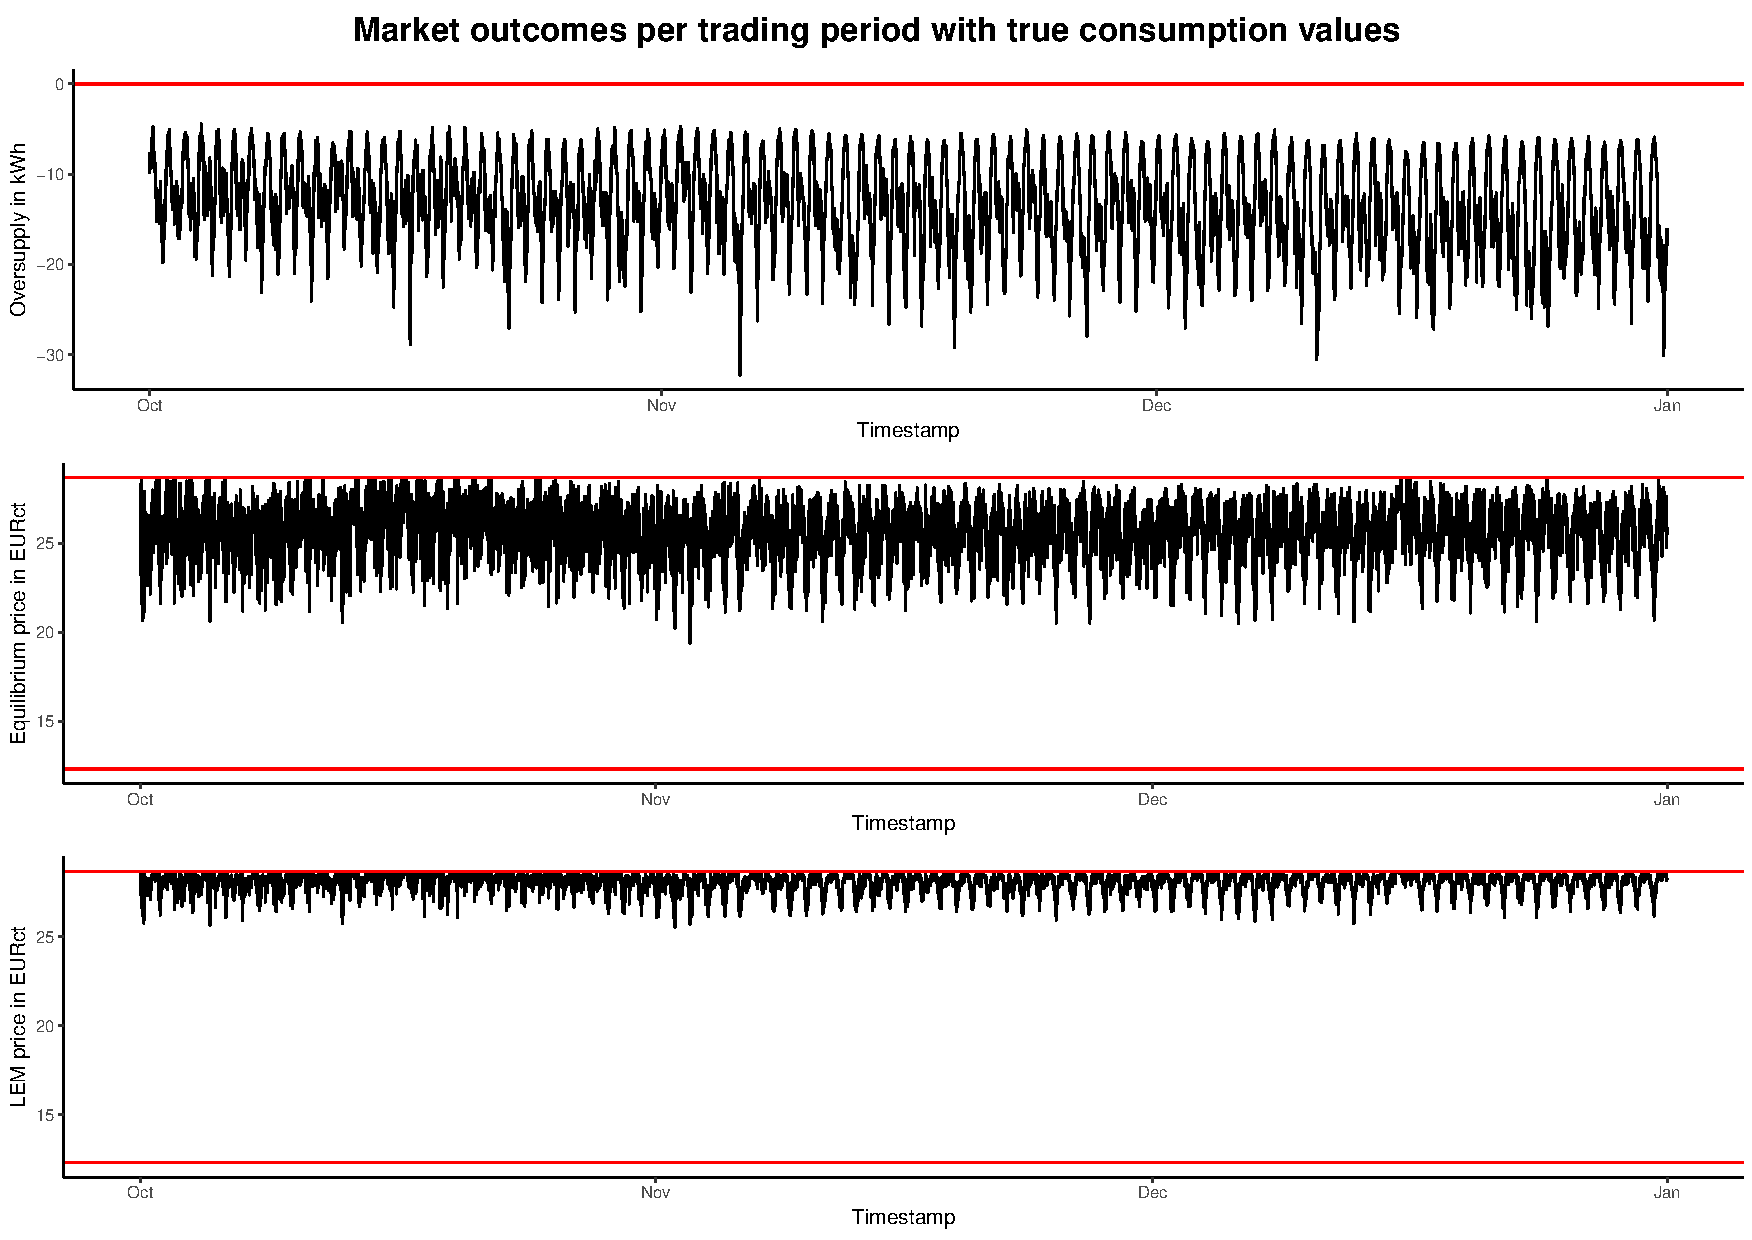
\includegraphics[width=\textwidth-1.1cm]{thesis/graphs/marketsimulation/marketoutcome_true_undersupply.pdf}
    \caption[Market outcomes simulated with undersupply and true values]{Market outcomes per trading period simulated with true values and an undersupply scenario. \quantnet\href{https://github.com/QuantLet/BLEM/tree/master/BLEMmarketSimulation}{BLEMmarketSimulation}}
    \label{Fig:marketoutcomes_true_under}
\end{figure}
%
\newpage
In summary, one can conclude that the market outcomes are the more favourable to consumers, the more locally produced energy is offered by prosumers. Assuming a closed double auction as market mechanism and zero-intelligence bidding behavior of market participants, oversupply reduces the LEM prices substantially leading to savings on the consumer side. On the other hand, prosumers will favor undersupply in the market as they profit from the high equilibrium prices while still being able to sell their surplus energy generation at the feed-in tariff without a loss compared to no LEM. Table~\ref{Tab:simulationresults} summarizes these results.


%%%%%%%%%%%
\subsubsection{Loss to consumers due to prediction errors}

To assess the adverse effect of prediction errors on the market outcomes, the LASSO-predicted energy consumption values per 15-minutes interval were used. The predictions of the model served as basis for the auction bids. After the true consumption in the respective trading period was observed, payments to settle over- or underestimation errors were made. That is, if a consumer bid with a higher amount than actually consumed, it still bought the full bid amount from the prosumers but had to sell the surplus to the energy utility over the grid at the feed-in tariff. On the other hand, if a consumer bid with a lower amount than actually consumed, it bought the bid amount from the prosumers but had to purchase the surplus energy consumption from the grid at the energy utility's tariff. Thus, prediction errors are costly as the consumer always has to clear the order at less favourable conditions than the equilibrium price provides.

Table~\ref{Tab:simulationresults} contrasts the results of the market simulation with true consumption values with the results of the market simulation with predicted values in three different supply scenarios. The equilibrium and LEM prices almost do not differ within the three scenarios whether the true or predicted consumption values are used. However, the prices between the scenarios differ substantially as was already indicated by Figures~\ref{Fig:marketoutcomes_true_balanced}, \ref{Fig:marketoutcomes_true_over} and \ref{Fig:marketoutcomes_true_under}. Furthermore, the average total revenue over the three month simulation period of the prosumers is largely unaffected by the use of true or predicted consumption values. This is not surprising as the revenue is a function of the equilibrium price, which is apparently largely unaffected by whether true or predicted consumption values are used, and the electricity produced, which is obviously completely unaffected by whether true or predicted consumption values are used. This might be different if also predicted instead of true production values were used in the market simulation.

What differs according to Table~\ref{Tab:simulationresults}, however, is the cost for consumers. The cost without LEM is on average across all consumers smaller when using predicted consumption values compared to using true consumption values. This can be explained by the LASSO model's tendency to underestimate and because correction payments for the prediction errors are not factored into this number (otherwise there would be no difference between ``true'' and ``predicted'' in all columns of the last table row). The average total cost for electricity consumption in the whole simulation period is with LEM higher when using predicted consumption values compared to using true consumption values. This is due to the above-mentioned need to settle prediction errors at unfavourable terms.
%
\begingroup\catcode`"=9
\begin{table}[ht]
{\footnotesize
    \csvreader[centered tabular=l|SSSSSS,
    before reading=\sisetup{round-mode=places,round-precision=2,round-integer-to-decimal},
     filter not strcmp={\thecsvinputline}{1},
     %filter expr={
      %test{\ifnumgreater{\thecsvinputline}{2}}},
    table head=
    \hline\hline
     \multirow{2}{2em}{\textbf{Mean}} & \multicolumn{2} {c}{\textbf{Balanced supply}} & \multicolumn{2} {c}{\textbf{Oversupply}} & \multicolumn{2} {c}{\textbf{Undersupply}}\\
     & \multicolumn{1} {c}{\textbf{true}} & \multicolumn{1} {c}{\textbf{predicted}} & \multicolumn{1} {c}{\textbf{true}} & \multicolumn{1} {c}{\textbf{predicted}} & \multicolumn{1} {c}{\textbf{true}} & \multicolumn{1} {c}{\textbf{predicted}}\\
    \hline,
    no head,
    separator=comma,
    respect all,
    late after line=\\,
    table foot=\hline \hline]
    {thesis/tables/average_outcomes.csv}{}%
    {\csvcolii & \csvcoliii & \csvcoliv & \csvcolv & \csvcolvi & \csvcolvii & \csvcolviii}}%
    \caption[Outcomes of market simulation for different supply scenarios]{Average results of the market simulation for three different supply scenarios. Prices are averaged across all trading periods. Revenues and costs for the whole simulation period are averaged across all prosumers and consumers respectively. \quantnet\href{https://github.com/QuantLet/BLEM/tree/master/BLEMevaluateMarketSim}{BLEMevaluateMarketSim}}
    \label{Tab:simulationresults}
\end{table}
\endgroup
%

The percentage loss induced by prediction errors is shown in Table~\ref{Tab:lossresults}. Depending on the supply scenario it ranges between abound 5~\% and 14~\%. These numbers have to be judged relative to the savings that are brought to consumers by the participation in a LEM. It turns out, that in the balanced supply scenario, the savings due to the LEM are almost completely offset by the loss due to prediction errors. As consumers profit more from a LEM the more oversupplied the local market is (and thus, the lower the equilibrium prices are), this is not the case in the oversupply scenario. Here, the savings are substantial and amount to about 130~\% which is almost ten times more than the percentage loss due to the prediction errors. The problem of the settlement structure for prediction errors becomes very apparent in the undersupply scenario. Here, the savings due to the LEM are more than offset by the loss due to prediction errors. Consequently, consumers would be better off to not participate in the LEM, and therefore, to not rely on imprecise predictions which make costly adjustment payments necessary.
%
\begingroup\catcode`"=9
\begin{table}[ht]
{\footnotesize
    \csvreader[centered tabular=l|SSS,
    before reading=\sisetup{round-mode=places,round-precision=2,round-integer-to-decimal},
    filter not strcmp={\thecsvinputline}{1},
    table head=
    \hline\hline
     \multicolumn{1} {l}{\textbf{Mean}} & \multicolumn{1} {c}{\textbf{Balanced supply}} & \multicolumn{1} {c}{\textbf{Oversupply}} & \multicolumn{1} {c}{\textbf{Undersupply}}\\
    \hline,
    no head,
    separator=comma,
    respect all,
    late after line=\\,
    table foot=\hline \hline]
    {thesis/tables/loss_outcomes.csv}{}%
    {\csvcolii & \csvcoliii & \csvcoliv & \csvcolv}}%
    \caption[Savings due to LEM and loss due to prediction errors]{Average savings for consumers due to LEM and average loss for consumers due to prediction errors in LEM. \quantnet\href{https://github.com/QuantLet/BLEM/tree/master/BLEMevaluateMarketSim}{BLEMevaluateMarketSim}}
    \label{Tab:lossresults}
\end{table}
\endgroup
%

This result is visualized in a more differentiated way in Figure~\ref{Fig:total_energycost}. The figure shows for each supply scenario, for each consumer, the total energy cost over the whole simulation period in (1) no LEM, in (2) a LEM with the use of predicted consumption values, and in (3) a LEM with the use of true consumption values. For each supply scenario the lower panel shows the percentage loss due to not participating in the LEM and the loss due to participating and using predicted consumption values compared to participating and using true consumption values. In the balanced scenario there are some consumers who would make a loss due to the participation in the LEM and relying on predicted values. For them, the loss due to no LEM (yellow bar) is smaller than the loss due to prediction errors (green bar). However, there are also 56 out of 88 consumer (64~\%) which profit from the participation in the LEM despite the costs induced by prediction errors. Due to the much lower equilibrium prices in the oversupply scenario, the LEM participation, here, is despite prediction errors profitable for all consumers. However, even in this scenario, the savings for the consumers are diminished by more than 10~\% which is quite substantial. On the contrary, in the undersupply scenario, the loss due to the prediction errors leaves the participation in the LEM for almost all consumers unprofitable. Merely three consumers would profit and have lower costs in a LEM despite prediction errors than without a LEM.

%
\begin{figure}[htbp]
    \centering
    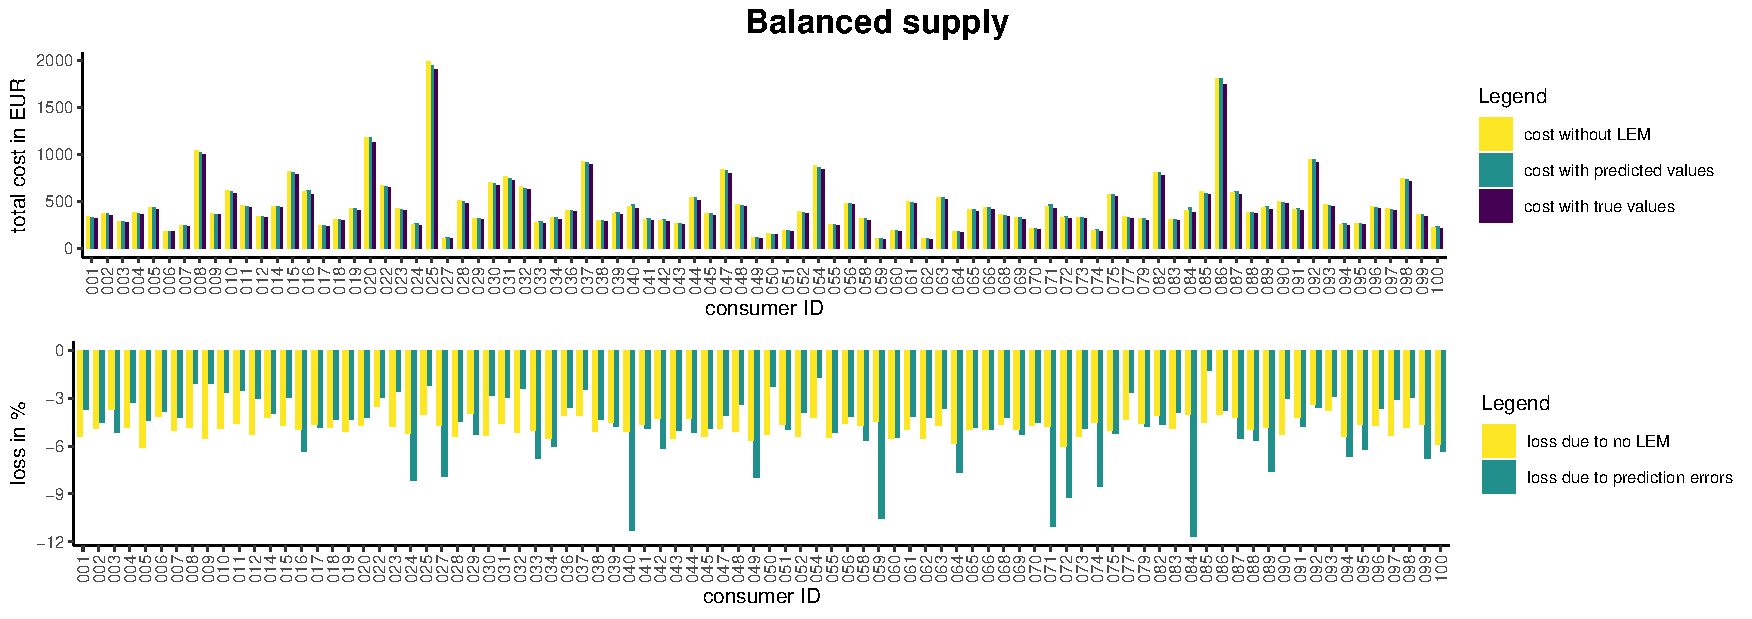
\includegraphics[width=\textwidth]{thesis/graphs/marketsimulation/totalenergycost_balanced.pdf}\\\vspace{.6cm}
    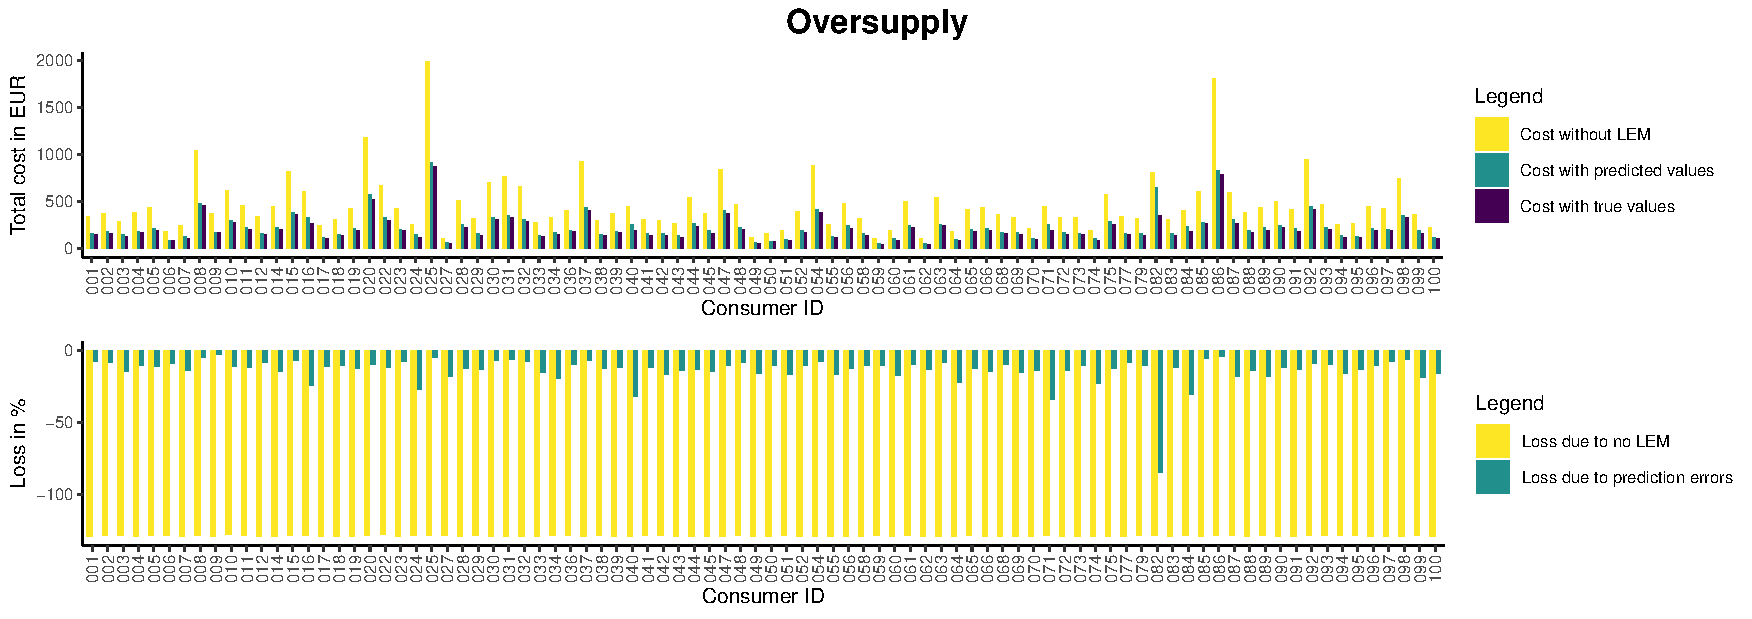
\includegraphics[width=\textwidth]{thesis/graphs/marketsimulation/totalenergycost_oversupply.pdf}\\\vspace{.6cm}
    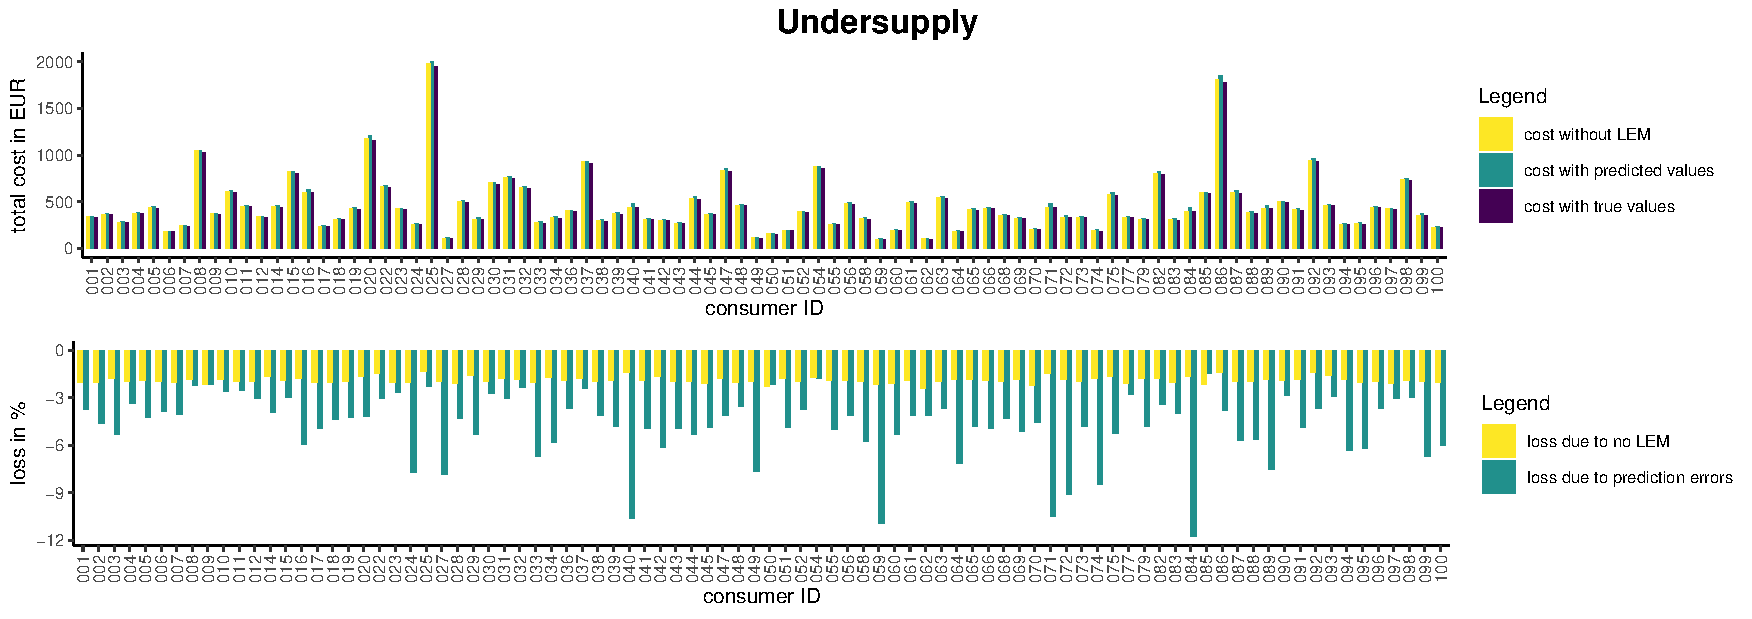
\includegraphics[width=\textwidth]{thesis/graphs/marketsimulation/totalenergycost_undersupply.pdf}
    \caption[Total energy cost to consumers in different supply scenarios]{Total energy cost to consumers from 01.10.2018 to 31.12.2017 in case of no LEM, LEM with true values, and LEM with predicted values in three different supply scenarios. \quantnet\href{https://github.com/QuantLet/BLEM/tree/master/BLEMevaluateMarketSim}{BLEMevaluateMarketSim}}
    \label{Fig:total_energycost}
\end{figure}
%

Overall, it becomes clear that prediction errors significantly lower the economic profitability for consumers. This, however, is often argued to be one of the main advantage of LEMs. The result is especially concerning in LEMs where locally produced energy is undersupplied. Here -- still assuming the closed double auction market mechanism and zero-intelligence bidding strategies -- the savings from the participation in the LEM are marginal. Therefore, the costs induced by prediction errors mostly outweigh the savings from the participation. This results in an overall loss for consumers due to the LEM which makes the participation economically irrational. Only in cases of substantial oversupply, the much lower equilibrium price compared to the energy utility's price compensates for the costs from prediction errors.

In conclusion, this means that LEMs with the market mechanism proposed in \citet{Mengelkamp:2018a} and the prediction accuracy of state-of-the-art energy forecasting techniques require substantial oversupply in the local market for a LEM to be beneficial to consumers.



%%%%%%%%%%%%%%%%%%%%%%%%
%%%   Implications   %%%
%%%%%%%%%%%%%%%%%%%%%%%%

\subsection{Implications for blockchain-based local energy markets}\label{Sec:Results;Subsec:Implications}

In light of these results, it remains open to derive implications and to propose potential adjustments for a smart contract market mechanism. After all, there are substantial advantages of LEMs which have been established in various studies as pointed out in Section~\ref{Sec:Intro;Subsec:Related} and which still make LEMs an attractive solution for the challenges brought about by the changing energy landscape. Adjustments mitigating the negative effect of prediction errors on the profitability of LEMs could address one or more of the following areas: first, the forecasting techniques employed, second, the demand and supply structure of the LEM, and third, the market mechanism used in the blockchain-based LEM.

The first and most intuitive option is to improve the forecasting accuracy with which the predictions, that serve as the basis of bids and asks, are made. The most obvious way to achieve such an improvement is the inclusion of more data. More data may hereby refer either to a higher resolution of recorded consumption respectively production data or to a wider range of data sources such as behavioral data of household members or data from smart appliances. A higher resolution of smart meter readings is already easily achievable. The smart meters installed by Discovergy that also supplied the data for the present research are capable of recording energy measurements up to every two seconds. However, data at such a fine granularity requires substantial data storage and processing capacities which are unlikely to be available in an average household. Especially, the training of prediction models with such vast amounts of input data points is computationally very resource intensive. The potential solution of outsourcing the data processing, the prediction model training, and the prediction making, however, introduces new data privacy concerns that are already a sensible topic within blockchain-based LEMs. \citet{Greveler:2012}, for example, found in 2012 that the data transmitted by Discovergy smart meters to Discovergy servers was not encrypted and easily interceptable. While this is most likely not possible anymore, it exemplifies the general vulnerability of internet-connected systems regarding data protection. Moreover, the authors showed that the data could be used to identify the television program which the household's LCD television was showingwith high precision. This highlights the sensibility of high-resolution energy consumption data as it allows for detailed inference of household members' behavior. The inclusion of behavioral data into prediction models such as the location of the person within their house or apartment and the inclusion of smart appliances' energy consumption (as done by \citet{Kong:2018}) and running schedules raises important privacy concerns as well. Using energy consumption data of several households, as done by \citet{Shi:2017}, again introduces privacy concerns. According to them, the data of several households in a neighborhood could be pooled to utilize common uncertainty within the data for model training and subsequently better prediction for individual households. However, this implies data sharing between households, which in relatively small LEMs cannot be guaranteed to preserve the anonymity of market participants, and thus, is not desirable from a data protection perspective. For all these reasons, it seems unlikely that in the near future much better predictions of the very short-term household energy consumption or production of individual households will be available.

The second option addresses the demand and supply structure in the blockchain-based LEM. As was shown in Section~\ref{Sec:Results;Subsec:Simulation}, the cost induced by prediction errors and their settlement is more than compensated in an oversupply scenario. Hence, employing LEMs only in a regional neighbourhood with energy production that surpasses energy consumption would mitigate the problem of unprofitability due to prediction errors as well. Where this is not possible, participation to the LEM could be restricted such that oversupply in a majority of trading periods is ensured. However, this seems to be an artificial market manipulation that most likely makes most of LEMs' advantages obsolete. Moreover, it is unclear on what basis the restriction to participate in the market should be grounded.

Lastly, the third option to mitigate the problem is the market mechanism and the prediction error settlement structure. A simple approach to reduce forecasting errors is to decrease the forecasting horizon. Thus, instead of having 15-minutes trading periods which also require 15-minutes ahead forecast, the trading periods could be shrunk to just 3 or 1 minute. This would increase the forecasting accuracy, and thereby, lead to lower costs due to the settlement of prediction errors. However, in a blockchain-based LEM more frequent market closings come at the cost of more computational resources needed for transaction verification and cryptographic block generation. Depending on the consensus mechanism used for the blockchain, the energy requirements for the computations that secure transactions and generate new blocks may be substantial. This, of course, is rather detrimental to the idea of promoting more sustainable energy generation and usage. Nevertheless, using consensus mechanisms based on identity verification of the participating agents may serve as a less computational, and thus energy intensive alternative, which might make shorter trading intervals reasonable.

Another, more radical approach might be to change the market mechanism of closed double auctions altogether and use an exposed market instead. Hereby, the energy consumption and production is settled in an auction after the true values are known, instead of in advance. This means, market participants submit just limit prices in their bids and asks without related amounts and the offers are matched in an auction in regular time intervals. Then, the electricity actually consumed and produced in the preceding period is settled according to the market clearing price. Related to this approach is a solution, where bidding is based on forecasted energy values, while the settlement is shifted by one period such that the actual amounts can be used for clearing. This approach, however, may introduce the possibility of fraud and market manipulation as agents can try to deliberately bid using false amounts. While in the smart contracted developed by \citet{Mengelkamp:2018a} funds needed to backup the bid are held as pledges until the contract is settled (this ensures the availability of the necessary funds to pay the bid), this would be senseless, if settlement is only based on actual consumption without considering the amount specified in the offer. However, the extent of this problem and ways to mitigate it should be assessed from a game theoretical perspective that is out of scope of the present research.

All in all, prediction errors have to be taken into account for future designs of blockchain-based LEMs. Otherwise, they may substantially lower the profitability and diminish the incentive to participate in a LEM for consumers. Also, the psychological component of having to rely on an unreliable prediction algorithm that may be more or less accurate depending on the household's energy consumption patterns seems unattractive. Even though possible solutions are not trivial and each come with certain trade-offs, there is room for future improvement of the smart contracts and the market mechanism they reproduce.

%%%%%%%%%%%%%%%%%%%%%%%%%%%%%%%%%%%%%%%%%%%%%%%%%%%%%%%%%%%%%%%%%


\section{Conclusion}\label{Sec:Conc}



%%%%%%%%%%%%%%%%%%%
%%%   Summary   %%%
%%%%%%%%%%%%%%%%%%%%

\subsection{Summary}\label{Sec:Conclusion;Subsec:Summary}

The present research aimed, first, to evaluate the prediction accuracy for household energy consumption and production using state-of-the-art forecasting techniques and, second, to assess the effect of prediction errors in a local energy market (LEM) using the market mechanism implemented in a smart contract by \citet{Mengelkamp:2018a}. Lastly, it aimed to infer the implications of the results for the future design of blockchain-based LEM.

For this purpose, first, the performance of two forecasting techniques, which were already successfully applied in previous research, was assessed. A LSTM recurring neural network and a LASSO regression model were fitted on 9 months of consumption respectively production data of German households recorded by smart meters in 3-minute intervals. These models were then used to predict energy consumption respectively production in 15-minute resolution one-step ahead for three months. The predictions were evaluated using several error measures and compared to a benchmark model (na\"ive persistence model). The LASSO model yielded the best results with an average MAPE across all consumer data sets of \textapprox17~\% and was subsequently used to make predictions for the succeeding market simulation. As all prediction models failed to produce satisfactory predictions on the production data, the market simulation used only true production values.

Secondly, the market mechanism implemented by \citet{Mengelkamp:2018a} was used to assess the effect of prediction errors on market outcomes in three different supply scenarios. The evaluation revealed that in a balanced supply and demand scenario the settlement cost due to prediction errors almost completely offset savings made possible by the participation in the LEM. In an undersupply scenario, the cost due to prediction errors even surpassed the savings and made market participation uneconomical. Only in a scenario with substantial oversupply, the savings brought to consumers by the participation in the LEM compensated the cost of prediction errors completely.

Thus, thirdly, further possible adjustments necessary for future blockchain-based LEM to mitigate this finding were discussed. Here, it was found that this problem would be only diminished but not eliminated by more accurate forecasts. Moreover, it seemed unlikely that the performance of prediction models could be greatly improved without including higher data resolution, behavioural variables, and data from smart appliances -- which still would not account for the unpredictability of human behaviour. Implementing blockchain-based LEM only in market setups with oversupply seems impractical and would most probably diminish the advantages of a LEM substantially. Therefore, the most promising approach seemed to be measures that address the market design. This mainly includes adjustments to the market mechanism, which can be two-fold: Either shorter trading periods could be introduced which in turn would reduce the forecasting horizon and therefore prediction errors or the auction mechanism could be altered to not use predicted consumption values to settle transactions.

Overall, the need to take prediction errors into consideration in the design of blockchain-based LEM market mechanisms became evident. This is due to the high uncertainty associated with individual households' energy consumption and therefore also net production patterns that limits the feasibility of accurate forecasts substantially.



%%%%%%%%%%%%%%%%%%%%%%
%%%   Discussion   %%%
%%%%%%%%%%%%%%%%%%%%%%

\subsection{Limitations}\label{Sec:Conclusion;Subsec:Discussion}

There are some limitations of the present work to point out. One major concern was that data from more smart meters and more context information about the data would have been desirable. Due to data protection legislation no information regarding locality of the households, the household characteristics or the type of power plant prosumer households used could be provided by Discovergy. This made it difficult to judge the suitability of certain data sets for the market simulation and required a detailed analysis of the energy recordings' patterns of every single data set provided. Also the large share of so declared prosumer data sets without any net energy production readings was unfortunate and unexplained. The large scale differences in the production capacities of the remaining prosumers with net energy production readings complicated the analysis of the market simulation further. Additionally, it would have been preferable to have absolute production and consumption data for prosumers instead of the net consumption respectively production. Nevertheless, this circumstance reflected real-world data availability and is something probably every implementation of blockchain-based LEM would have to deal with. This fact, however, highlights the necessity to improve net demand forecasting as has been already pointed out in previous research as well \citep[e.g.,][]{Meer:2018, Hong:2016}.

The prediction performance of the LSTM model was slightly surprising. The author would have expected better results, especially compared to the LASSO regression model. Here, a major constrained for more elaborate model architectures, the inclusion of more data points and more sophisticated and granular hyperparameter tuning was computing resources. The computing resources available were either not optimized for large scale neural network training (i.e., a lack of graphical processing units (GPUs) capable of tensor operations) or prohibitively expensive to use and, thus, exceeding the free trial credits for computing resources (i.e., the Google Cloud Platform Free Tier).

Especially, the prediction of production data could have been much better in view of the dedicated research fields that exist for the forecasting of electricity production by different type of plants. However, this knowledge could not be adequately put to use in the present work as the households' type of production plants was not known and would have had to be inferred from net production patterns with a high degree of uncertainty. The evaluation of the predictions on production data also suffered from the unavailability of relative error measures due to the frequent occurence of zero values. The usage of MAPE or NRMSE with the plants production capacity as denominator (as suggested by \citet{Hoff:2013}) would have solved this problem. However, this again would have required knowledge about the maximum capacity of the production plants which was not available.

Another promising approach to quantify error measures in the presence of sudden unexpected peaks is the ramp score as utilized in wind energy forecasting and developed on the basis of a swinging door algorithm \citep[e.g.,][]{Bianco:2016, Florita:2013}. This may be useful to include in future similar work.

Finally, it is to mention that the market simulation did not account for taxes or fees, especially grid utilization fees, which can be a substantial share of the total electricity cost of households. Moreover, the simulation does not take into account compensation costs for blockchain miners that reimburses them for the computational cost they bear. The modeling of this cost and potential distribution schemes among market participants is definitively needed in future research on blockchain-based energy markets \citep[see also][]{Mengelkamp:2018a}.



%%%%%%%%%%%%%%%%%%%
%%%   Outlook   %%%
%%%%%%%%%%%%%%%%%%%

\subsection{Outlook and future research}\label{Sec:Conclusion;Subsec:Outlook}

Naturally, future research concerned with blockchain-based LEM should take into account the potential cost of prediction errors. This implies a focus on market mechanisms and prediction error settlement structures that do not make participation in the LEM uneconomical. A special focus on this issue has to be put in situations with an undersupply of locally produced energy. A further field of research that already is picking up in sophistication and amount is the forecast of individual household energy consumption and production. However, as the results of this field are still nowhere close to the forecasting accuracy of aggregated consumption forecasting, there is still room for improvement and refinement of existing prediction techniques. Any advancements made in the prediction of individual households' energy patterns also benefits the blockchain-based LEM research as energy forecasts most likely will play a role in their use cases. Furthermore, to the author's knowledge there has been no simulation of blockchain-based LEM with actual consumption and production data conducted. Doing so on a private blockchain with the market mechanism coded in a smart contract should be the next step for the assessment of potential technological and conceptual weaknesses.

Previous research has shown that blockchain technology and smart contracts can play a valuable role in tackling the challenges of a changing energy landscape. The research in this thesis emphasizes, however, that advancement on this front cannot be made without a holistic approach that takes all components of blockchain-based LEM into account. Simply assuming that reasonably accurate energy forecasts for individual households will be available once the technical challenges of implementing a LEM on a blockchain are solved, may steer research into a wrong direction and lead us to miss the opportunity to quickly move into the direction of a more sustainable and less carbon-intensive future.


%%%%%%%%%%%%%%%%%%%%%%%%%%%%%%%%%%%%%%%%%%%%%%%%%%%%%%%%%%%%%%%%%



% -----------------------
% --- Acknowledgement ---
% -----------------------
\newpage
\phantomsection\addcontentsline{toc}{section}{Acknowledgement}
\section*{Acknowledgement}

I would like to thank Discovergy GmbH for the kind provision of their smart meter data.




% ------------------
% --- literature ---
% ------------------
\newpage
\begingroup
    \spacing{1}
    \phantomsection\addcontentsline{toc}{section}{References}
    \bibliography{thesis/10_literature.bib}
\endgroup


% ----------------
% --- appendix ---
% ----------------
\newpage
\begin{appendices}

% figures
\renewcommand\thefigure{A\arabic{figure}}
\setcounter{figure}{0}

\section*{Appendix \hypertarget{AppA:Figures}{A}: Figures} \label{App:Figures}

\subsection*{\hypertarget{AppA1:Figures:Excludedc}{A1} Excluded consumer data sets}\label{AppA1:Figures:Excludedc}

\begin{centering}
\begin{figure}[!htbp]
        \includegraphics[width=\textwidth-0.85cm]{thesis/graphs/timeseries/c021_cons.pdf}\vspace{0.3cm}
        \includegraphics[width=\textwidth-0.85cm]{thesis/graphs/timeseries/c046_cons.pdf}
\end{figure}
\begin{figure}[!htbp]
        \includegraphics[width=\textwidth-0.85cm]{thesis/graphs/timeseries/c053_cons.pdf}\vspace{0.3cm}
        \includegraphics[width=\textwidth-0.85cm]{thesis/graphs/timeseries/c057_cons.pdf}
\end{figure}
\begin{figure}[!htbp]
        \includegraphics[width=\textwidth-0.85cm]{thesis/graphs/timeseries/c078_cons.pdf}\vspace{0.3cm}
        \includegraphics[width=\textwidth-0.85cm]{thesis/graphs/timeseries/c080_cons.pdf}
        \caption[Consumer data sets excluded due to peculiarities in the consumption patterns]{Consumer data sets excluded due to peculiarities in the consumption or production patterns. \quantnet\href{https://github.com/QuantLet/BLEM/tree/master/BLEMplotEnergyData}{BLEMplotEnergyData}}
\end{figure}
\end{centering}


\subsection*{\hypertarget{AppA2:Figures:Excludedp}{A2} Excluded consumer data sets}\label{AppA2:Figures:Excludedp}

\begin{centering}
\begin{figure}[H]
        \includegraphics[width=\textwidth-0.85cm]{thesis/graphs/timeseries/p012_prod&cons.pdf}\vspace{0.3cm}
        \includegraphics[width=\textwidth-0.85cm]{thesis/graphs/timeseries/p015_prod&cons.pdf}
        \caption[Prosumer data sets excluded due to peculiarities in the production patterns]{Prosumer data sets excluded due to peculiarities in the production patterns. \quantnet\href{https://github.com/QuantLet/BLEM/tree/master/BLEMplotEnergyData}{BLEMplotEnergyData}}
\end{figure}
\end{centering}


\subsection*{\hypertarget{AppA3:Figures:transform}{A3} Normalized log-consumption data}\label{AppA3:Figures:transform}

\begin{centering}
\begin{figure}[!htbp]
        \includegraphics[width=\textwidth-0.85cm]{thesis/graphs/c020_density.pdf}
        \caption[Exemplary energy consumption distribution before and after transformation]{Consumer 020's density estimate of energy consumption values before and after transformation. \quantnet\href{https://github.com/QuantLet/BLEM/tree/master/BLEMplotScaling}{BLEMplotScaling}}
\end{figure}
\end{centering}


\subsection*{\hypertarget{AppA4:Figures:erroranalysis}{A4} Error analysis of consumer 027}\label{AppA4:Figures:erroranalysis}

\begin{centering}
\begin{figure}[H]
    \includegraphics[width=\textwidth]{thesis/graphs/evaluation/c027_squarederrors.pdf}
    \caption[Squared relative errors of predictions by LSTM model on consumer 027]{Squared relative errors of predictions by LSTM model on data set of consumer 027. \quantnet\href{https://github.com/QuantLet/BLEM/tree/master/BLEMevaluateEnergyPreds}{BLEMevaluateEnergyPreds}}
\end{figure}
\end{centering}


\subsection*{\hypertarget{AppA5:Figures:heatmaps_p}{A5} Error evaluation of predictions on production data}\label{AppA5:Figures:heatmaps_p}

\begin{figure}[H]
    \centering
    \includegraphics[width=\textwidth]{thesis/graphs/evaluation/p_heatmap_MAE.pdf}
    \includegraphics[width=\textwidth]{thesis/graphs/evaluation/p_heatmap_RMSE.pdf}
    \includegraphics[width=\textwidth]{thesis/graphs/evaluation/p_heatmap_MASE.pdf}
    \caption[Heatmaps of error measures for production values]{Heatmaps of MAE, RMSE, and MASE scores for the prediction of production values per prosumer data set. \quantnet\href{https://github.com/QuantLet/BLEM/tree/master/BLEMevaluateEnergyPreds}{BLEMevaluateEnergyPreds}}
\end{figure}


\subsection*{\hypertarget{AppA6:Figures:producer_all}{A6} Overview of prosumers' energy production time series}\label{AppA6:Figures:producer_all}

\begin{figure}[H]
    \centering
    \includegraphics[width=\textwidth]{thesis/graphs/marketsimulation/producers_all.pdf}
    \caption[Energy production time series of prosumers relevant for market simulation]{Energy production time series of prosumer data sets that are potentially relevant for the market simulation in the time period from 01.10.2017 00:00 to 01.01.2018 00:00. \quantnet\href{https://github.com/QuantLet/BLEM/tree/master/BLEMmarketSimulation}{BLEMmarketSimulation}}
\end{figure}


\newpage
\subsection*{\hypertarget{AppA7:Figures:marketsimulation_pred}{A7} Market simulation with predicted values}\label{AppA7:Figures:marketsimulation_pred}

\begin{figure}[H]
    \centering
    \includegraphics[width=\textwidth-.85cm]{thesis/graphs/marketsimulation/marketoutcome_pred_balanced.pdf}\\\vspace{.6cm}
    \includegraphics[width=\textwidth-.85cm]{thesis/graphs/marketsimulation/marketoutcome_pred_oversupply.pdf}
\end{figure}
    
\begin{figure}[H]
    \centering
    \includegraphics[width=\textwidth-.85cm]{thesis/graphs/marketsimulation/marketoutcome_pred_undersupply.pdf}
    \caption[Market outcomes simulated in three supply scenarios with predicted values]{Market outcomes per trading period simulated with predicted values in a balanced, an oversupply, and an undersupply scenario. \quantnet\href{https://github.com/QuantLet/BLEM/tree/master/BLEMmarketSimulation}{BLEMmarketSimulation}}
\end{figure}

%%%%%%%%%%%%%%%%%%%%%%%%%%%%%%%%%%%%%%%%%%%%%%%%%%%%%%%%%%%%


% tables
\newpage
\renewcommand\thetable{B\arabic{table}}
\setcounter{table}{0}

\section*{Appendix \hypertarget{AppB:Tables}{B}: Tables}\label{App:Tables}

\subsection*{\hypertarget{AppB1:Tables:totalcons}{B1} Summary statistics of total energy consumption and production} \label{AppB1:Tables:totalcons}

\begingroup\catcode`"=9
\begin{table}[ht]
{\footnotesize
    \csvreader[centered tabular=l|SSSSSS,
    before reading=\sisetup{round-mode=places,round-precision=2,round-integer-to-decimal},
    filter not strcmp ={\thecsvinputline}{1},
    table head=
    \hline\hline
     & \multicolumn{1} {c}{\textbf{Min}} & \multicolumn{1} {c}{\textbf{Q1}} & \multicolumn{1} {c}{\textbf{Median}} & \multicolumn{1} {c}{\textbf{Mean}} & \multicolumn{1} {c}{\textbf{Q3}} & \multicolumn{1} {c}{\textbf{Max}}\\
    \hline,
    no head,
    separator=comma,
    respect all,
    late after line=\\,
    table foot= \hline \hline]
    {thesis/tables/summarystats_total.csv}{}%
    {\csvcolii & \csvcoliii & \csvcoliv & \csvcolv & \csvcolvi & \csvcolvii & \csvcolviii}}%
    \caption[Summary statistics of households' total consumption and production in 2017]{Summary statistics of households' total consumption and production in kWh for 2017. \quantnet\href{https://github.com/QuantLet/BLEM/tree/master/BLEMdescStatEnergyData}{BLEMdescStatEnergyData}}
\end{table}
\endgroup


\subsection*{\hypertarget{AppB2:Tables:avg_errM_wMedian}{B2} Prediction model performance across consumer data sets} \label{AppB2:Tables:avg_errM_wMedian}

\begingroup\catcode`"=9
\begin{table}[ht]
{\footnotesize
    \csvreader[centered tabular=l|SSSSSSS,
    before reading=\sisetup{round-mode=places,round-precision=2,round-integer-to-decimal},
    filter not strcmp={\thecsvinputline}{1},
    table head=
    \hline\hline
     \multicolumn{1} {l}{\textbf{Model}} & \multicolumn{1} {c}{\textbf{MAE}} & \multicolumn{1} {c}{\textbf{RMSE}} & \multicolumn{1} {c}{\textbf{MAPE}} & \multicolumn{1} {c}{\textbf{MdAPE}} & \multicolumn{1} {c}{\textbf{NRMSE}} & \multicolumn{1} {c}{\textbf{NRMdSE}} & \multicolumn{1} {c}{\textbf{MASE}}\\
    \hline,
    no head,
    separator=comma,
    respect all,
    late after line=\\,
    table foot=\hline \hline]
    {thesis/tables/avg_errorMeasures_corrected.csv}{}%
    {\csvcolii & \csvcoliii & \csvcoliv & \csvcolv & \csvcolvi & \csvcolvii & \csvcolviii & \csvcolix}}%
    \caption[Mean of error measures across all 82 consumer data sets]{Mean of error measures for the prediction of energy consumption across all 82 consumer data sets including the median absolute percentage error (MdAPE) and normalized root median squared error (NRMdSE). \quantnet\href{https://github.com/QuantLet/BLEM/tree/master/BLEMevaluateEnergyPreds}{BLEMevaluateEnergyPreds}}
\end{table}
\endgroup


\subsection*{\hypertarget{AppB3:Tables:medain_errM_prod}{B3} Prediction model performance across prosumer data sets} \label{AppB3:Tables:medain_errM_prod}

\begingroup\catcode`"=9
\begin{table}[ht]
{\footnotesize
    \csvreader[centered tabular=l|SSS,
    before reading=\sisetup{round-mode=places,round-precision=2,round-integer-to-decimal},
    filter not strcmp={\thecsvinputline}{1},
    table head=
    \hline\hline
     \multicolumn{1} {l}{\textbf{Model}} & \multicolumn{1} {c}{\textbf{MAE}} & \multicolumn{1} {c}{\textbf{RMSE}} & \multicolumn{1} {c}{\textbf{MASE}}\\
    \hline,
    no head,
    separator=comma,
    respect all,
    late after line=\\,
    table foot=\hline \hline]
    {thesis/tables/median_errorMeasures_p.csv}{}%
    {\csvcolii & \csvcoliii & \csvcoliv & \csvcolv}}%
    \caption[Median of error measures for all 12 prosumer data sets]{Median of error measures for the prediction of energy production across all 12 prosumer data sets. \quantnet\href{https://github.com/QuantLet/BLEM/tree/master/BLEMevaluateEnergyPreds}{BLEMevaluateEnergyPreds}}
\end{table}
\endgroup


%%%%%%%%%%%%%%%%%%%%%%%%%%%%%%%%%%%%%%%%%%%%%%%%%%%%%%%%%%%%%%%%%%%%%%%%%%%%%%%%%%%%

% code
\newpage

\section*{Appendix \hypertarget{AppC:Code}{C}: Code}\label{AppC:Code}

% define line spacing = 1
\renewcommand{\baselinestretch}{1}

\subsection*{\hypertarget{AppC1:Code:API}{C1} Java REST API Client} \label{AppC1:Code:API}
The code is adapted from the Discovergy Java API demo client\footnote{The demo client can be downloaded here: \url{https://api.discovergy.com/docs/binaries/DiscovergyAPIClient.zip} (last accessed: 08.09.2018).}.

\subsubsection*{DiscovergyApi.java}\unskip
\inputminted[
breaklines,
obeytabs=true,
tabsize=2
]{java}{code/DiscovergyApi.java}
\unskip

\subsubsection*{DiscovergyApiClient.java}\unskip
\inputminted[
breaklines,
obeytabs=true,
tabsize=2
]{java}{code/DiscovergyApiClient.java}
\unskip

\subsubsection*{Readings.java}\unskip
\inputminted[
breaklines,
obeytabs=true,
tabsize=2
]{java}{code/Readings.java}
\end{appendices}



% --------------------------------------------
% --- last page: Declaration of Authorship ---
% --------------------------------------------

\newpage
\thispagestyle{empty}
%{\Large{\bf Declaration of Authorship}}\vspace{0.5cm}

\section*{Declaration of Authorship}

I, Michael Kostmann, hereby confirm that I have not previously submitted the present work for other examinations. I authored this Master's thesis independently and without use of others than the indicated sources. All passages which are literally or in general matter taken out of publications or other sources are marked as such. I understand that violations of these principles will result in proceedings regarding deception or attempted deception.
\\\vspace{0.5cm}

\noindent Berlin, November 07, 2018 \\\vspace{0.1cm}

\noindent Michael Kostmann



\end{document}

%%%%%%%%%%%%%%%%%%%%%%%%%%%%%%%%%%%%%%%%%%%%%%%%%%%%%%